%\documentclass[preprint,review,12pt]{elsarticle}
\documentclass[times,final]{elsarticle}
%\documentclass[times,twocolumn,final,longtitle]{elsarticle}\usepackage{amssymb}
\usepackage{amsmath}
\usepackage{color}
\usepackage{graphics}
\usepackage{epsfig,epstopdf}
\usepackage{graphicx}
\usepackage{epsfig}
%\usepackage{amsfonts,amssymb,amsthm,epsfig,epstopdf,titling,url,array}
%\usepackage{caption}
%\usepackage{subcaption}
\usepackage{float}
%\usepackage{natbib}
%\usepackage{cite}
%\usepackage{lineno,hyperref}
%\modulolinenumbers[5]
\usepackage{color}
%\usepackage{showlabels}
\usepackage[normalem]{ulem}
\usepackage{epsf}


\usepackage{listings}

%
%
%2345678901234567890123456789012345678901234567890123456789012345678901234567890


% (Jie Li?:) Ici, on definit trois macros

% la premiere est une macro avec deux parametres: le premier specifie
%       la largeur, le second le nom du fichier en EncasulatedPostscript ou se
%       trouve ton dessin.

\def\epsfx#1#2{\leavevmode\epsfxsize=#1 \epsfbox{#2}}

% la seconde est une macro avec deux parameters: mais le premier specifie
%       la hauteur, le second le nom en EncasulatedPostscript ou se
%       trouve ton dessin.

\def\epsfy#1#2{\leavevmode\epsfysize=#1 \epsfbox{#2}}

% la troisieme est une macro avec trois parameters: le premier specifie
%       la larheur, le second la hauteur, le troisieme le nom de fichier
%       en EncasulatedPostscript ou se trouve ton dessin

\def\epsfxy#1#2#3{\leavevmode\epsfxsize=#1 \epsfysize=#2 \epsfbox{#3}}


\newcommand\lgawebsite{{\tt ftp://ftp.jussieu.fr/jussieu/labos/lmm}}
% For Notes sections
\newcommand\subn{\paragraph{}}

\newcommand{\refeq}[1]{(\ref{#1})}
\newcommand{\reff}[1]{(\ref{#1})}

\newcommand{\trema}{\"}
%boldface letters

\newcommand\A{{\bf a}}
\newcommand\B{{\bf b}}
\newcommand\C{{\bf c}}
\newcommand\D{{\bf d}}
\newcommand\E{{\bf e}}
\newcommand\I{{\bf i}}
\newcommand\J{{\bf j}}
\newcommand\K{{\bf k}}
\newcommand\G{{\bf g}}
\newcommand\M{{\bf m}}
\newcommand\N{{\bf n}}
\renewcommand\P{{\bf p}}
\newcommand\Q{{\bf q}}
\newcommand\R{{\bf r}}
\newcommand\F{{\bf f}}
\newcommand\T{{\bf t}}
\newcommand\U{{\bf u}}
\newcommand\ut{{\tilde u}}
\newcommand\vt{{\tilde v}}
\newcommand\wt{{\tilde w}}
\newcommand\V{{\bf v}}
\newcommand\W{{\bf w}}
\newcommand\X{{\bf x}}
\newcommand\Y{{\bf y}}
\newcommand\Z{{\bf z}}

\renewcommand\AA{{\bf A}}
\newcommand\BB{{\bf B}}
\newcommand\CC{{\bf C}}
\newcommand\DD{{\bf D}}
\newcommand\EE{{\bf E}}
\newcommand\FF{{\bf F}}
\newcommand\MM{{\bf M}}
%\newcommand\NN{{\bf N}}
%\renewcommand\NN{{\typeout{Warning ! } \bf WARNING NN NOT AVAIL}}
\newcommand\II{{\bf I}}
\newcommand\JJ{{\bf J}}
\newcommand\KK{{\bf K}}
\newcommand\GG{{\bf G}}
\newcommand\PP{{\bf P}}
\newcommand\RR{{\bf R}}
\renewcommand\SS{{\bf S}}
\newcommand\TT{{\bf T}}
\newcommand\UU{{\bf U}}
\newcommand\UT{{\bf \tilde u}}
\newcommand\XX{{\bf X}}
\newcommand\YY{{\bf Y}}
\newcommand\ZZ{{\bf Z}}

\newcommand\MMM{{\cal M}}
\newcommand\NNN{{\cal N}}

\newcommand\derta{\partial_{t_1}}
\newcommand\dertb{\partial_{t_2}}
\newcommand\dert{\partial_t}
\newcommand\derx{\partial_x}
\newcommand\dery{\partial_y}
\newcommand\derz{\partial_z}
\newcommand\derr{\partial_r}
\newcommand\derth[1]{\frac{\partial #1}{\partial \theta}}
\newcommand\dera{\partial_\alpha}
\newcommand\derb{\partial_\beta}
\newcommand\deri[1]{ \frac{\partial{ #1}}{\partial{x_i}} }
\newcommand\derj[1]{ \frac{\partial{ #1}}{\partial{x_j}} }
\newcommand\derxj{ \frac{\partial}{\partial{x_j}} }
\newcommand\derxi{ \frac{\partial}{\partial{x_i}} }
\newcommand\dertt[1]{ \frac{\partial{ #1}}{\partial t} }
\newcommand\derft{ \frac{\partial}{\partial t} }
\newcommand\dertj[1]{\frac{\partial^2 #1}{\partial x_j^2}}
\newcommand\jac[2]{\frac{\partial(#1,#2)}{\partial(x,z)}}

\newcommand\derd[1]{\frac{D #1}{Dt}}
\newcommand\romandt[1]{\frac{{\rm d} #1}{{\rm d}t}}

\newcommand\der[2]{\frac{\partial #1}{\partial #2}}
\newcommand\pori[2]{\frac{\partial #2}{\partial #1}}
\newcommand\derbrack[2]{\frac{\partial}{\partial #2}\left[ #1 \right]}

\newcommand\romander[2]{\frac{{\rm d} #1}{{\rm d}#2}}

\newcommand\grad{\nabla}

% Greek

\newcommand\eps{\epsilon}
\newcommand\ii{{\rm i}}
\newcommand\om{{\omega}}

\newcommand\porh[1]{\frac{\partial H ( {\cal S} )}{\partial #1}}

\newcommand\be{\begin{equation}}
\newcommand\nd{\end{equation}}
\newcommand\bed{\begin{displaymath}}
\newcommand\ndd{\end{displaymath}}
\newcommand\hb[1]{\hbox{\hskip 3 pt #1 \hskip 3 pt} }
\newcommand\ba{\begin{array}}
\newcommand\ea{\end{array}}

% Miscellaneous

\newcommand\Order{{\cal O}}
\newcommand\cijk{C_{i,j,k}}
\newcommand\paris{{\sc ParisSimulator }}

\newcommand\bea{\begin{eqnarray}}
\newcommand\nda{\end{eqnarray}}

% A
\renewcommand\Re{{\rm Re}\,}
\newcommand\re{{\rm Re}\,}
\newcommand\We{{\rm We}\,}
\newcommand\Ra{{\rm Ra}\,}
\newcommand\Ma{{\rm Ma}\,}
\newcommand\Bo{{\rm Bo}\,}
\newcommand\Ca{{\rm Ca}\,}
\newcommand\Oh{{\rm Oh}\,}
\newcommand\La{{\rm La}\,}
%\newcommand\Nu{{\rm Nu}\,}
\newcommand\At{{\rm At}\,}


% or B:
%\input{macros-df.tex}
%\undefine\neq{ {n_{\rm eq}}}

\newcommand\ubar{{\bar u}}
%\def\includegraphics#1{}
%\def\scalebox#1{}

\def\Ubar{{\bf U}}
\def\vbar{{\bf v}}
\def\abar{{\bf a}}
\def\rbar{{\bf r}}
\def\xbar{{\bf x}}
\def\nbar{{\bf n}}
\def\ombar{{\bf \omega}}
\def\psibar{{\bf \psi}}
\def\Abar{{\bf \Psi}}
\def\ubar{{\bf u}}
\def\gamabar{{\bf \gamma}}
\def\betabar{{\bf \beta}}

% You cannot have number in the middle of a tex name: \gr1or is 
% equivalent to \gr 1or
% So I remove these two for the moment. (Stephane)
%\def\gr1or{{\grad \Bigl({1 \over r}\Bigr)}}
%\def\nd1or{{{\partial \over \partial n'} \Bigl({1 \over r}\Bigr)}}
\def\pint{{\int \!\!\!\!\!\! -}}
\def\shat{{\hat s}}
%\def\nhat{{\hat n}}
\def\nhat{{\bf n}}
\def\jhat{{\hat \jmath}}
\def\khat{{\hat k}}
\def\that{{\hat t}}
\def\bhat{{\hat b}}
\def\grad{{\nabla}}

%\def\Ma{{\it Ma}}
\def\dero{{\bf {}}}

\def\u{{u}}

\def\v{{v}}


\journal{Computers and Fluids}




%\usepackage[colorlinks,bookmarksopen,bookmarksnumbered,urlcolor=red]{hyperref} %dvips
%\newcommand\BibTeX{{\rmfamily B\kern-.05em \textsc{i\kern-.025em b}\kern-.08em T\kern-.1667em\lower.7ex\hbox{E}\kern-.125emX}}
\newcommand {\red}[1]{{{#1}}}
\newcommand {\blue}[1]{{{#1}}}
\newcommand {\magenta}[1]{{{#1}}}
\newcommand {\cyan}[1]{{{#1}}}
%\newcommand\textcolor[1]{\red{#1}}

%\newcommand {\red}[1]{{\color{red}{#1}}}
%\newcommand {\blue}[1]{{\color{blue}{#1}}}
%\renewcommand {\red}[1]{{}}
%\renewcommand {\blue}[1]{{#1}}



\begin{document}

%\verso{Given-name Surname \textit{etal}}

\begin{frontmatter}

%% Title, authors and addresses

%% use the tnoteref command within \title for footnotes;
%% use the tnotetext command for the associated footnote;
%% use the fnref command within \author or \address for footnotes;
%% use the fntext command for the associated footnote;
%% use the corref command within \author for corresponding author footnotes;
%% use the cortext command for the associated footnote;
%% use the ead command for the email address,
%% and the form \ead[url] for the home page:
%%
%% \title{Title\tnoteref{label1}}
%% \tnotetext[label1]{}
%% \author{Name\corref{cor1}\fnref{label2}}
%% \ead{email address}
%% \ead[url]{home page}
%% \fntext[label2]{}
%% \cortext[cor1]{}
%% \address{Address\fnref{label3}}
%% \fntext[label3]{}

\title{A momentum-conserving, consistent, Volume-of-Fluid method for incompressible flow on staggered grids}

%% use optional labels to link authors explicitly to addresses:
%% \author[label1,label2]{}
%% \address[label1]{}
%% \address[b]{}
\author[b]{D. Fuster}
\author[b]{T. Arrufat}
\author[f]{M. Crialesi-Esposito}
\author[a]{Y. Ling}
\author[b,d]{L. Malan}
\author[b]{S. Pal}
\author[e]{R. Scardovelli}
\author[label1]{G. Tryggvason}
\author[b]{S. Zaleski}
\address[b]{Sorbonne Universit\'e et CNRS, \\Institut Jean Le Rond d'Alembert, UMR 7190, Paris, France}
%\address[c]{CNRS, UMR 7190, Institut Jean Le Rond d'Alembert, F-75005, Paris, France}
\address[f]{CMT-Motores T\'ermicos, Universitat Polit\'ecnica de Val\'encia, Camino de Vera, s/n, Edificio 6D, Valencia, Spain}
\address[d]{InCFD, Dept. of Mechanical Engineering, University of Cape Town, South Africa}
\address[e]{ DIN - Lab. di Montecuccolino, Universit\`a di Bologna, I-40136 Bologna, Italy}
\address[label1]{Mechanical Engineering, Johns Hopkins University, Baltimore, USA}
\address[a]{Dept. of Mechanical Engineering, Baylor University, Waco, TX, USA} 


\begin{abstract}
%% Text of abstract
   The computation of flows with large density contrasts is notoriously   difficult. To alleviate the difficulty we consider a consistent mass and   momentum-conserving discretization of the Navier-Stokes   equation. Incompressible flow with capillary forces is modelled   and the discretization is performed on a staggered grid of Marker   and Cell type. The Volume-of-Fluid method is used to track the   interface and a Height-Function method is used to compute surface   tension. The advection of the volume fraction is performed using   either the Lagrangian-Explicit / CIAM (Calcul d'Interface Affine par Morceaux)    method or the Weymouth and Yue (WY)   Eulerian-Implicit method. The WY method conserves fluid mass to machine    accuracy provided incompressiblity is satisfied which leads to    a method that is both momentum and mass-conserving.     To improve the stability of these methods   momentum fluxes are advected in a manner ``consistent'' with the   volume-fraction fluxes, that is a discontinuity of the momentum is   advected at the same speed as a discontinuity of the density. To   find the density on the staggered cells on which the velocity is   centered, an auxiliary reconstruction of the density is   performed. The method is tested for a droplet without surface   tension in uniform flow, for a droplet suddenly accelerated in a   carrying gas at rest at very large density ratio without viscosity   or surface tension, for the Kelvin-Helmholtz instability, for a   falling raindrop and for an atomizing flow in air-water conditions.

\end{abstract}

\begin{keyword}
Multiphase Flows \sep Navier-Stokes Equations \sep Volume of Fluid \sep Surface Tension \sep Large Density Contrast
%Multiphase Flows ; Navier-Stokes equations ; Volume of Fluid ; Surface Tension ; large density contrast
 %% keywords here, in the form: keyword \sep keyword

%% PACS codes here, in the form: \PACS code \sep code

%% MSC codes here, in the form: \MSC code \sep code
%% or \MSC[2008] code \sep code (2000 is the default)

\end{keyword}


\end{frontmatter}
%% \linenumbers

%% main text
\newcommand\division[1]{\subsection{#1}}
\newcommand\subdivision[1]{\subsubsection{#1}}
\newcommand\onlybook[1]{{}}
\newcommand\opus{article}
\newcommand\reduit[1]{#1}
\newcommand\LLL{{\cal L}}
\section{Introduction} 
Multiphase flows abound in nature, but their stable and accurate computation remains elusive in many cases.
As a case in point, many numerical methods used for two-phase incompressible flow are
strongly unstable for large density contrasts and large Reynolds numbers. 
Experience with such simulations shows that the presence of
surface tension is an aggravating factor. The large density contrasts that are of interest are 
 air/water or gas/liquid-metal, with $\rho_l/\rho_g$ of the order of $10^3$ or $10^4$.
The large density contrasts are a difficulty whether one deals with any of the three major
interface advection methods, Level-Set, Volume-of-Fluid (VOF) or Front-Tracking, or with combinations 
such as CLSVOF.  (The term density contrast is perferable to density ratio since it encompasses ratios both much larger than one and much smaller than one.)

Several methods have been used to alleviate the high-density-contrast difficulties.
It has been observed by several authors that making the momentum-advection method conservative improves the situation. 
%The rationale for this is that momentum conservation is a ``physical'' property of the methods. 
For incompressible flow, momentum-conserving methods have been initially proposed by \cite{rudman98},
and by several other authors since \cite{bussmann2002modeling,desjardins10,raessi12,le13,Vaudor:2017ip}.
These methods have been shown to
improve the stability of the numerical results in various situations. In particular, liquid-gas flows
 with very contrasted densities, as for example in the the process of atomization,
cause serious problems that are resolved by using momentum-conserving methods. 
In that case another oft-suggested solution is to increase the number of 
equations from the standard four equations to five, six or seven equations, 
by introducing new field variables in each phase. 
The addition of one more density $\rho_i$, momentum $\rho_i \U_{i}$ or energy variable
$\rho_i e_i$  increases  the number of equations. 
The authors of ref. \cite{Saurel99} used seven equations, 
those of \cite{allaire02} used five equations and six equations were used in \cite{Pelanti14}. 
The last three references also use a momentum-conserving formulation. 
Several authors, including some of those cited above, have argued that the difficulty may come from 
gas velocities of order $u_g$ being mixed with liquid densities of order $\rho_l$. 
Both the $\rho_l$ and $u_g$ scales are large and the appearance of an unphysical $\rho_l u_g^2$ dynamic pressure scale could create numerical pressure fluctuations of the same order and unphysical pressure spikes, 
as the one nicely illustrated in \cite{xiao2012large} in the front part of a
suddenly accelerated small droplet. One way of avoiding this unphysical mixture of liquid and gas
quantities is to extrapolate liquid and gas pressure and velocity in the ``other'' phase, 
as in the ghost fluid method. This extrapolation strategy was used successfully in \cite{Xiao:2014vs}. 

It may be argued that a way to avoid this numerical diffusion of liquid and gas quantities is to advect 
the volume fraction and the conserved quantities that depend on it (density, momentum and energy) in a consistent manner.
In incompressible flow in which we specialise in this paper, it means that the volume fraction and momentum
or velocity must be advected in the same way. This is equivalent to request 
that the discontinuity of the Heaviside function $H$, marking the phase transition,
should be advected at the same speed as the discontinuity in momentum. 
This can be expressed by the following consistency requirement: 
if momentum is initially exactly proportional to volume fraction, 
it should remain so after advection. 
We call such a method VOF-consistent.

To satisfy this requirement the idea is to solve
the advection equation for momentum with the same numerical scheme that
is used for the VOF color function.
{This consistency property minimizes the unphysical transfer of momentum from one phase to another due to the differences in the numerical schemes used. The consistency is especially important
when dealing with fluids with a large density contrast where a small numerical momentum transfer from the dense phase to the light phase results in large numerical errors in the velocity field which in turn creates numerical instabilities.}

In this work, we present a modification of the classical 
momentum-preserving scheme proposed by \cite{rudman98}
for the case of a staggered grid and VOF method. We also focus more on 
the consistency requirement between VOF and momentum advection, and only 
partially conserve momentum in the scheme. This will illustrate mostly the benefit
of using a consistent advection scheme. 

The paper is organized as follow: the second section deals with the continuum mechanics formulation 
for incompressible flow and sharp interfaces. Section 3 describes our numerical method, starting
with an overview of already-known methods for spatial discretization, time-stepping, and VOF advection. We 
continue with the new momentum advection-VOF-consistent method. Section 4 is devoted to tests of the 
method, followed by a conclusion. 

Among the authors, Gretar Tryggvason, Ruben Scardovelli, Yue Stanley Ling and Stephane
Zaleski have been involved in the construction of the base of the
ParisSimulator VOF and Front-Tracking code that was used to implement
and test the ideas in this paper. ParisSimulator is itself based on a
Front-Tracking code developed by Gretar Tryggvason, Sadegh Dabiri and
Jiacai Lu.  Daniel Fuster was involved in the development of the
Momentum Conserving method with consistent VOF advection, with help
from Tomas Arrufat, Leon Malan and Yue Stanley Ling.  The falling
raindrop testing and the corresponding figures were done by Tomas
Arrufat for the CIAM method and Sagar Pal for the WY
method. The atomisation testing was done by Marco
Crialesi-Esposito. 


% sections "equations" and "method".

\section{Navier--Stokes equations with interfaces} 
\label{nse}

We model flows with sharp interfaces defined implicitly by a characteristic function $H(\X,t)$
defined such that fluid 1 corresponds to $H=1$ and fluid 2 to $H=0$. The viscosities $\mu$
and densities $\rho$ are calculated as an average
\be
\mu = \mu_1 H + \mu_2 (1-H)\,, \qquad \rho = \rho_1 H + \rho_2 (1 - H) \,. 
\label{muH}
\nd
There is no phase change so the interface, 
almost always a smooth differentiable surface $S$, advances at the speed of the 
flow, that is $V_S=\U\cdot \N$ where $\U$ is the local fluid velocity 
and $\N$ a unit normal vector perpendicular to the interface. Equivalently 
the interface motion can be expressed in weak form
\be
\dert H + \U \cdot \grad H = 0 \,, 
\label{interfadv}
\nd
which expresses the fact that the singularity of $H$, located on $S$, moves at velocity $V_S=\U\cdot \N$. 
For incompressible flows, which we will consider in what follows, we have
\be
\nabla \cdot \U = 0 \,.
\label{divu}
\nd
The Navier--Stokes equations for incompressible, Newtonian flow with surface tension may 
conveniently be written in operator form
\be
 \dert (\rho \U) = \LLL(\rho,\U) - \grad p \label{nse1}
\nd
where 
$
\LLL =  \LLL_{\rm conv} + \LLL_{\rm diff} +   \LLL_{\rm cap} + \LLL_{\rm ext}
$
so that the operator $\LLL$ is the sum of advective, diffusive, capillary force and
external force terms. The first two terms are 
\be
\LLL_{\rm conv} = -\grad \cdot ( \rho \U  \U )\,, \qquad \LLL_{\rm diff} =  \grad \cdot \DD \,,
\nd
where $\DD$ is a stress tensor whose expression for incompressible flow is
\be
\DD = \mu \left[ \nabla\U + (\nabla\U)^T \right] \,,
\nd
where $\mu$ is computed from $H$ using (\ref{muH}). 
The capillary term is
\be
\LLL_{\rm cap} =  {\sigma \kappa \delta_S \N} \,,  \qquad \kappa = 1/R_1 + 1/R_2 \,,
\nd
where $\sigma$ is the surface tension, $\N$ is the unit normal perpendicular to the interface,
$\kappa$ is the sum of the principal curvatures and $\delta_S$ is 
a Dirac distribution concentrated on the interface.  
We assume a constant surface tension value $\sigma$. Finally
$\LLL_{\rm ext}$ represents external forces such as gravity. 

% These equations may be coupled with a thermal energy equation
% {
% \be
% C_p (\dert T + \U \cdot \grad T) = \dot{q} \,, 
% \nd
% where $C_p=\rho c_p $ is the heat capacity per unit volume, $c_p$ the constant pressure specific heat, $T$ the temperature and $\dot{q}$ thermal diffusion. Note that for the purpose of this paper, we neglect viscous heating in the thermal energy equation. We also assume a divergence free velocity field with no mass transfer between phases (no phase change). We assume Fourier's law to model thermal energy diffusion $\dot{q} = \grad \cdot k\grad T$, with $k$ the thermal conductivity. Similar to momentum conservation, it is possible to write a conservative formulation for thermal energy conservation
% \be
% \dert (C_p T) + \grad \cdot (C_p T \U) = \grad \cdot k\grad T \,.
% \nd
% }
% Using the energy-conserving formulation above and advecting consistenly $C_p$ and $T$ may also be benficial for the 
% stability and accuracy of the code. 

\section{Method} % See below

\subsection{Spatial discretization}

\begin{figure}
\begin{center}
    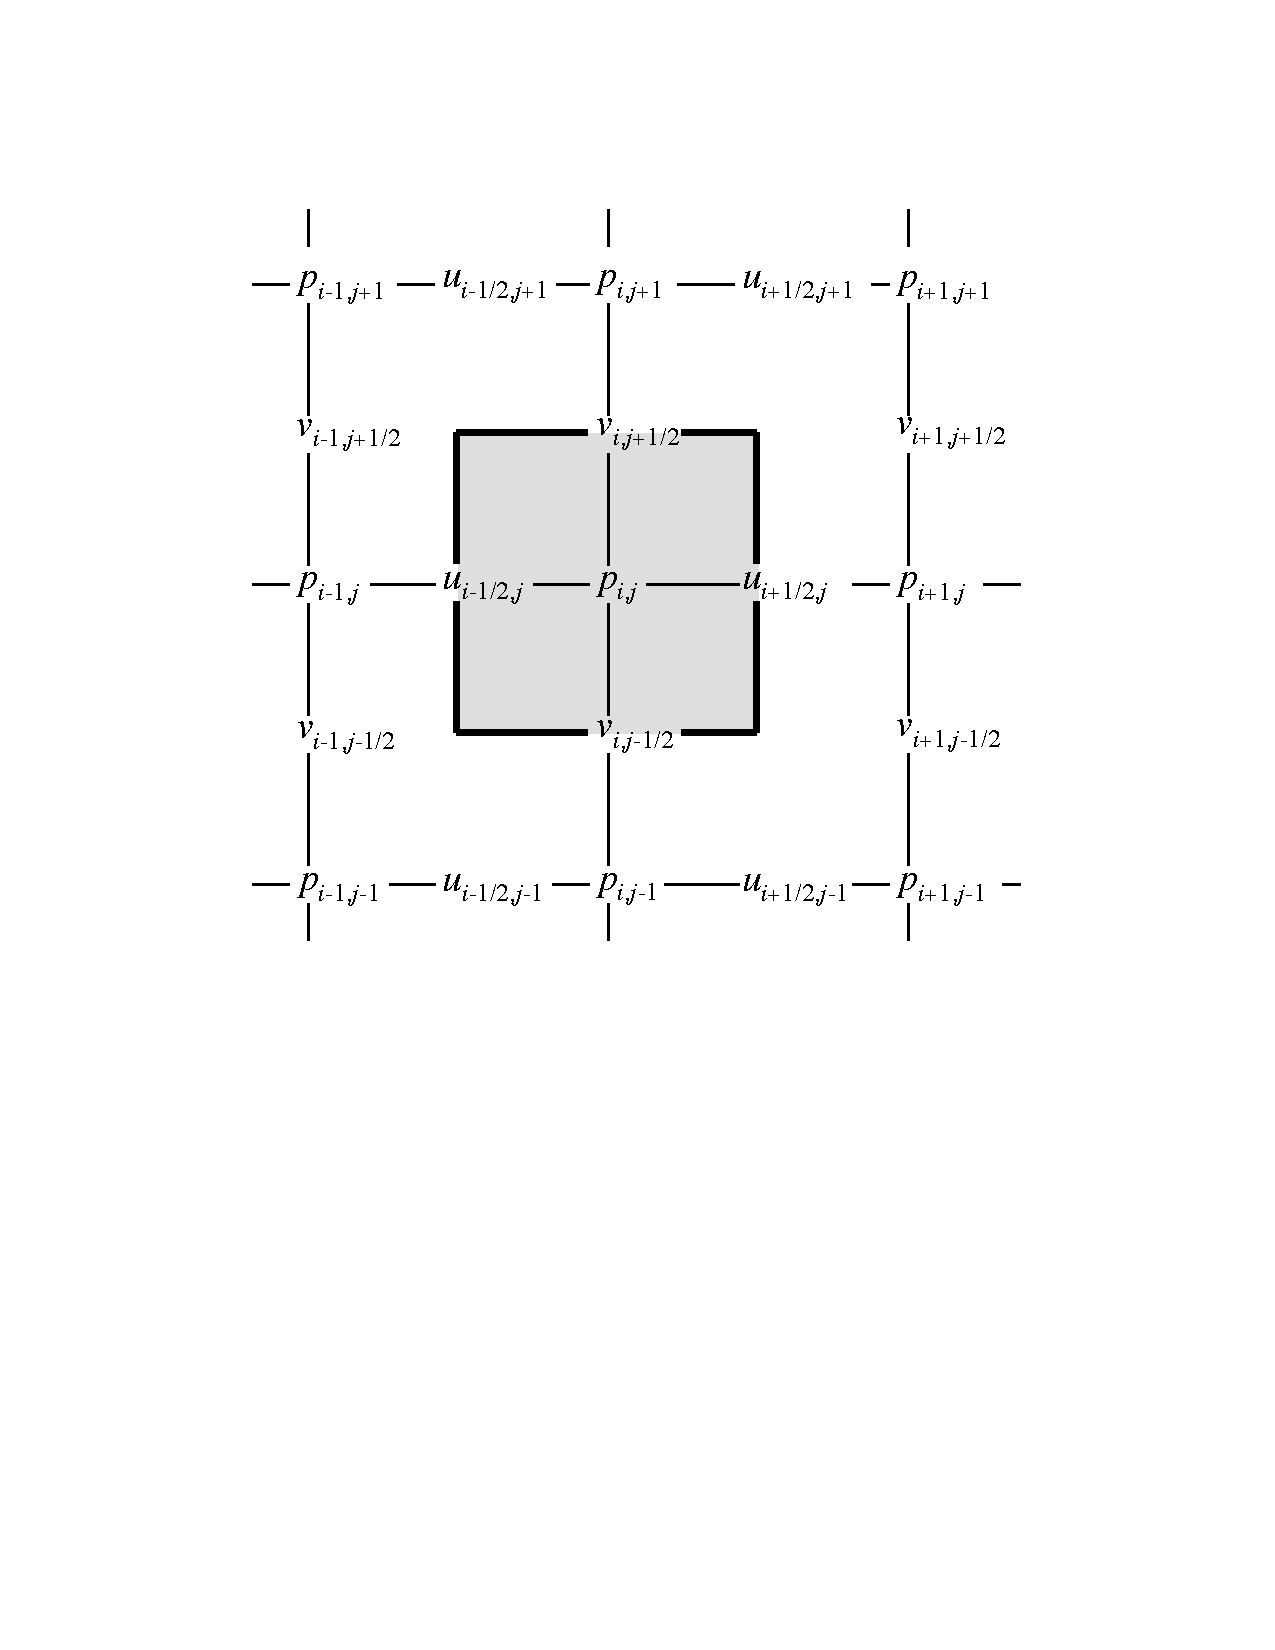
\includegraphics[width=0.45 \textwidth]{Figures/figure3-1.pdf}
\end{center}
\caption{Representation of the staggered spatial discretisation. The pressure $p$ is assumed to 
be known at the center of the control volume outlined by a thick solid line. The horizontal 
velocity component $u_1=u$ is stored in the middle of the left and right edges of this control 
volume and the vertical velocity component $u_2=v$ in the middle of the top and bottom edges.}
\label{stag-grid}
\end{figure}

We assume a regular cubic or square grid. This can be easily
generalized to rectangular or cuboid grids, and with some efforts to
quadtree and octree grids. We also use staggered velocity and pressure
grids. This makes our method more complex than it would be on a
collocated grid. 

The staggered grid is represented in Figure \ref{stag-grid}. In a staggered
grid discretization of the advection equation
the control volumes of the velocity components $u_1$ and $u_2$ are shifted with respect to the
control volume surrounding the pressure $p$.
The use of staggered control volumes has the advantage of
suppressing neutral modes often observed in collocated methods but
leads to more complex discretizations (see \cite{Tryggvason11} for a
more detailed discussion.) The control volumes for $u_1$ and $u_2$ are
shown on Figure \ref{Mac-u-v}. This type of staggered representation
is easily generalized to three dimensions. In what follows we shall
use these control volumes for the velocity or momentum components.

Using the staggered grid leads to a compact expression for the continuity equation
\eqref{divu}
\begin{equation}
{u_{1;i+1/2,j,k}- u_{1;i-1/2,j,k}\over \Delta x}+ 
{u_{2;i,j+1/2,k}- u_{2;i,j-1/2,k}\over \Delta y}+
{u_{3;i,j,k+1/2}- u_{3;i,j,k-1/2}\over \Delta z}=0,
\label{cont2}
\end{equation}
\begin{figure}
\begin{center}{\scalebox{0.4}{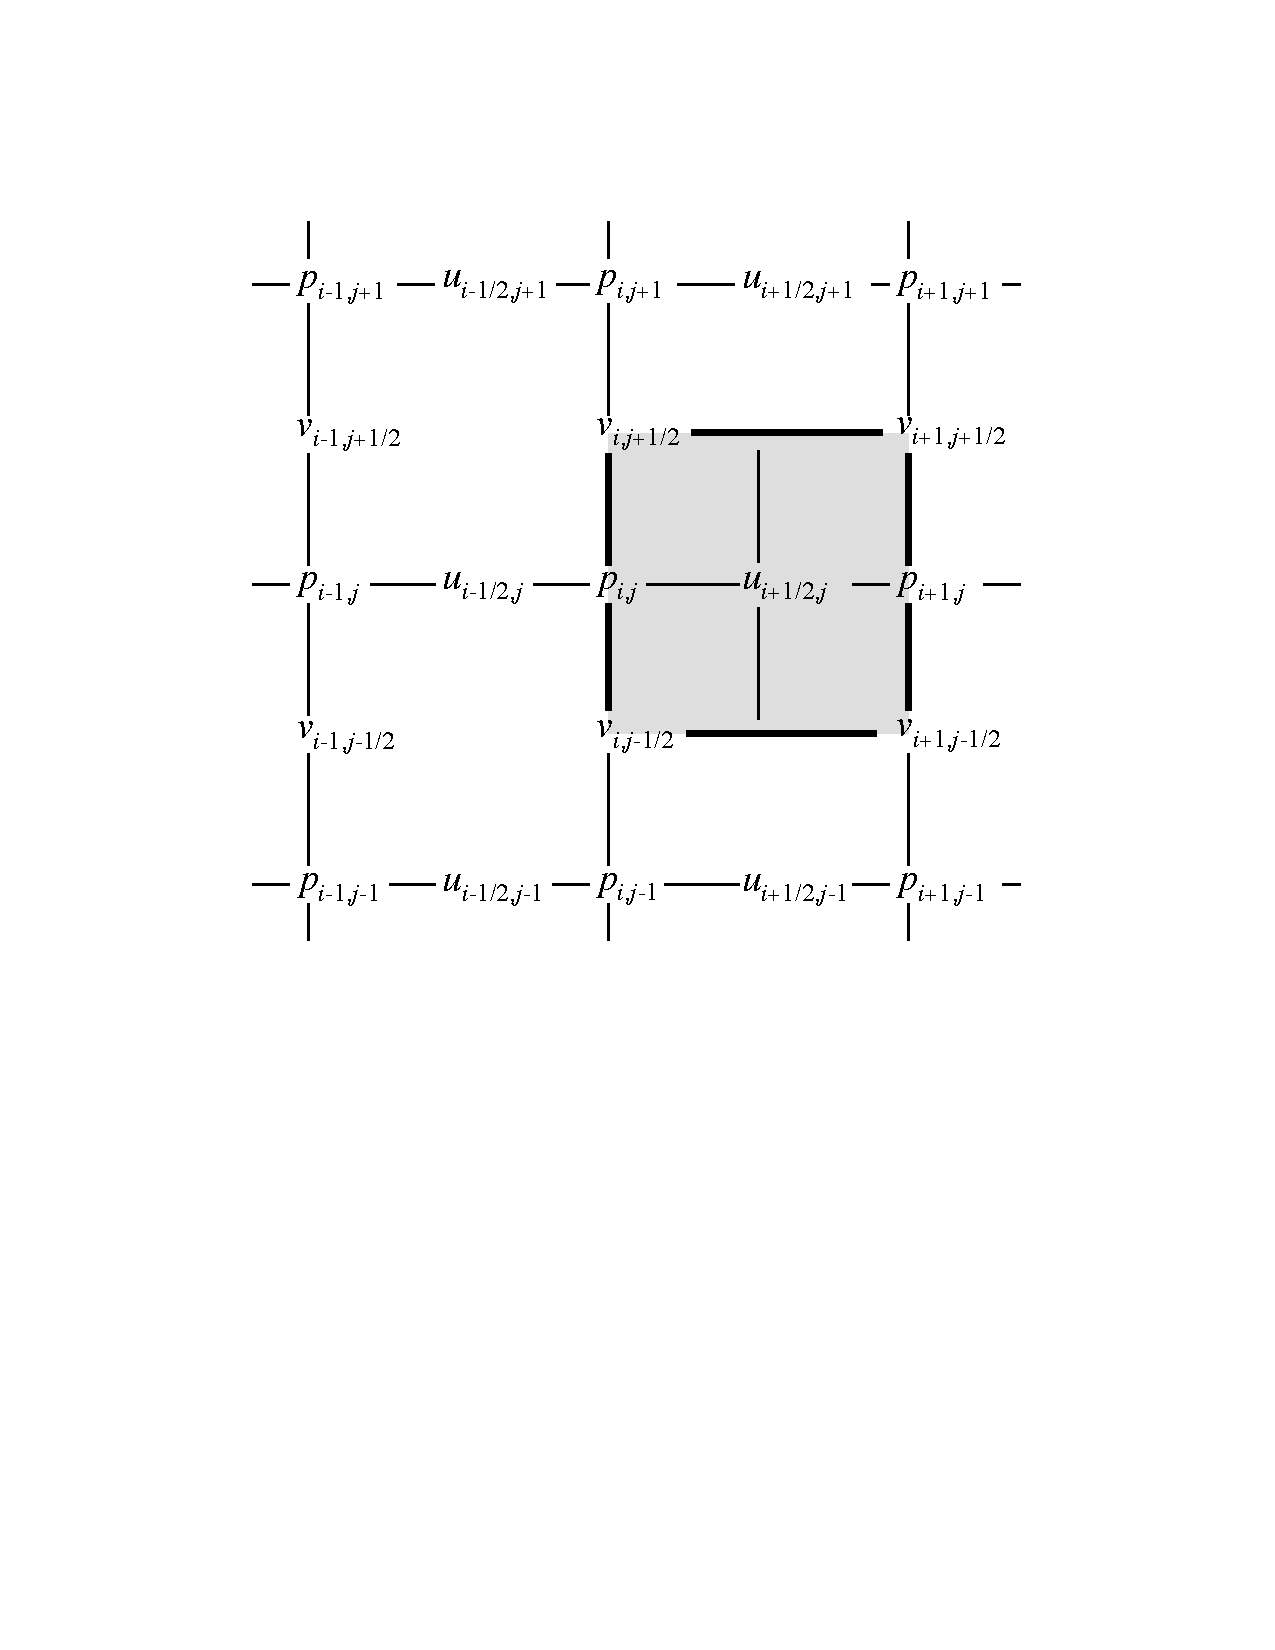
\includegraphics{Figures/figure3-2a.pdf}} \quad
\scalebox{0.4}{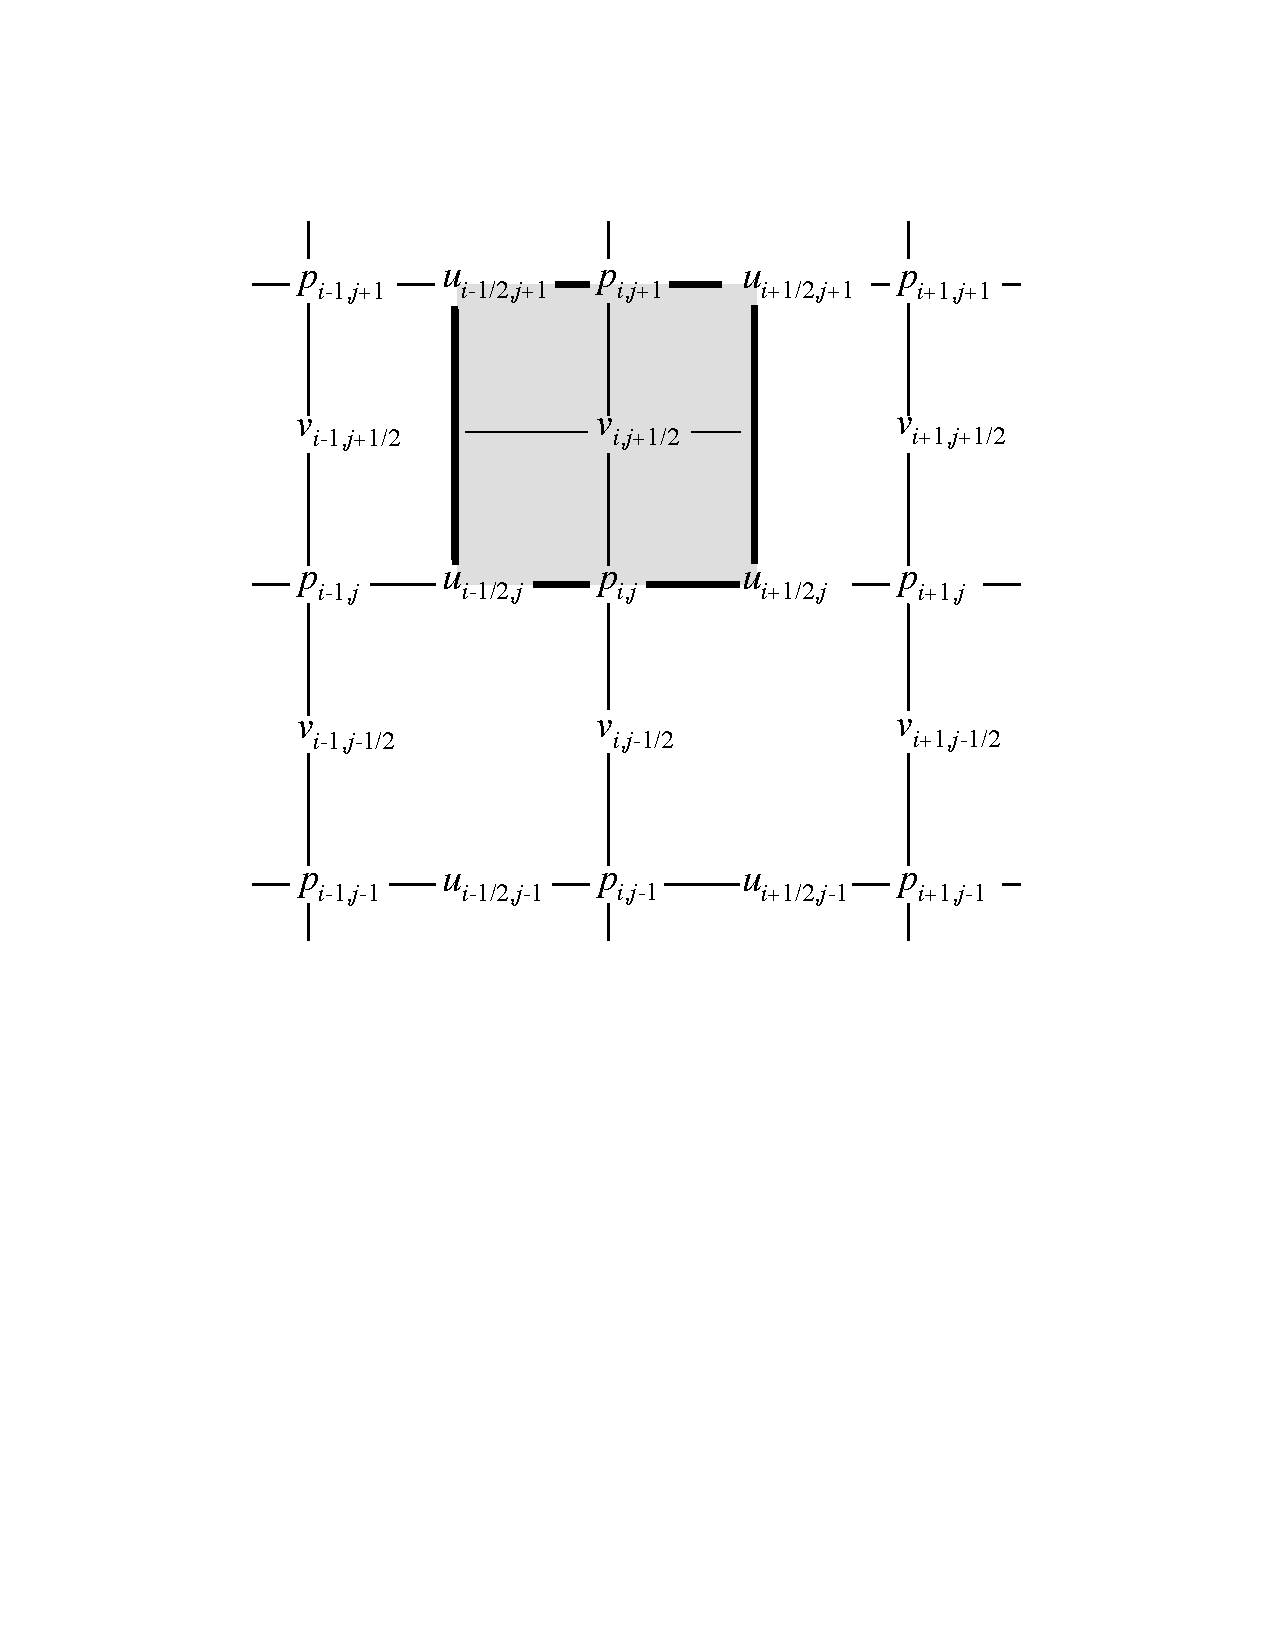
\includegraphics{Figures/figure3-2b.pdf}}  }\\
    (a) \hskip 5cm (b)
\end{center}
\caption{The control volumes for the $u_1=u$ and the $u_2=v$ velocity components are displaced 
half a grid cell to the right (horizontal velocities) and to the top (vertical velocities). Here the 
indices show the location of the stored quantities. Thus, half indices indicate those variables 
stored at the edges of the pressure control volumes.}
\label{Mac-u-v}
\end{figure}
In what follows, we shall use the notation $f=m\pm$, with the integer index $m=1,2,3$,
to note the face of any control volume located in the positive or negative Cartesian direction $m$, 
and $\N_f$ for the normal vector of face $f$ pointing outwards of the control volume.
On a cubic grid the spatial step is
$\Delta x = \Delta y = \Delta z = h$ so the continuity equation becomes
\be
\grad^h \cdot \U = \sum_{m=1}^3 (u_{m+} + u_{m-})/h =0 \,, 
\label{incompdisc3}
\nd
where $u_f=u_{m\pm}= \U \cdot \N_f $ is the velocity normal to face $f$. 
The discretization of the interface location is performed using a VOF method.
VOF methods typically attempt to solve approximately equation (\ref{interfadv}) 
which involves the Heaviside function $H$, whose integral 
in the cell $\Omega$ indexed by $i,j,k$ defines the volume fraction 
$\cijk$ from the relation
\be
h^3 \,\cijk  =\int_\Omega  H  {\rm d}\X \,.
\nd
$\cijk$ represents the fraction of the cell labelled by $i,j,k$ filled with fluid 1, 
taken to be the reference fluid. 
It is worth noting that in the staggered grid setup,
the control volume for $p$ is also the control volume for other scalar quantities,
such as $\rho$ and $H$.

\subsection{Time Marching}

The volume fraction field is updated as
\be
C^{n+1} = C^{n} + \LLL_{\rm VOF}(C^{n},\U^{n}\tau/h) \,,
\label{cnp1}
\nd
where $\LLL_{VOF}$ represents the operator that updates the Volume of Fluid data
given the velocity field. Once volume fraction is updated, the
velocity field is updated in a couple of steps. A projection method is first used, 
in which a provisional velocity field $\U^*$ is computed
\be
\rho^{n+1} \U^* = \rho^n \U^{n} +  \tau \LLL^h_{\rm conv}(\rho^{n},\U^{n}) + \tau \left[\LLL^h_{\rm diff}(\mu^{n},\U^{n}) +  \LLL^h_{\rm cap}(C^{n+1}) + \LLL^h_{\rm ext}(C^{n+1})\right] \label{conspredictedvel}
\nd
It goes without saying that the above operators depend on the discretization steps 
$\tau$ and $h$ as well as the fluid parameters. 
The discussion of the $\LLL^h_{\rm conv}$ operator is the main point of this paper. 
In the second step, the projection step, the pressure gradient force 
is added to yield the velocity at the new time step
\be
\U^{n+1} = \U^* - \frac{\tau }{\rho^{n+1}} \nabla^h p \,. 
\label{fotm}
\nd
The pressure is determined by the requirement that the 
velocity at the end of the time step must be divergence free
\be
\grad^{h} \cdot \ubar^{n+1}=0 \,,
\label{cont-eq1}
\nd
which leads to a Poisson-like equation for the pressure
\be
\grad^h \cdot \frac{\tau }{\rho^{n+1}} \nabla^h p =  \grad^h \cdot \U^* \,.
\nd

\subsection{Volume-Of-Fluid}
\label{vof}
We follow the usual VOF method and will only detail the necessary steps to illustrate the momentum advection method based on the VOF method in the next section. Moreover we will use in this section a rescaling of the space and time variables so that the cell size is 1, and the time step is also 1. All velocities are then rescaled to $u^\prime = u \tau / h$. Because of this space rescaling and in these new units, $\cijk$ is also the measure of the volume of reference fluid in cell $i,j,k$.


\subsubsection{Volume initialisation}

Before any VOF interface tracking is performed, the field of $\cijk$
values must be initialized. We use the {\sc Vofi} library described in \cite{bna2015numerical} and \cite{bna2016vofi}. 
This allows a high-accuracy numerical integration of the measure of the fluid volumes. 

\subsubsection{Normal vector determination} 

The VOF method proceeds in two steps, reconstruction and advection. In
the reconstruction step, one attempts to obtain the ``best'' possible representation of the interface 
using Volume of Fluid data $\cijk$. The best representation is usually the one with the smallest 
reconstruction error for objects such as circles or ellipses, but issues of continuity and robustness 
at low resolution may also be considered. In the work reported here 
we use a standard method  described in \cite{Tryggvason11}.  In each cell cut by the interface
one first determines the interface normal
vector $\N$, then one solves the problem of finding a plane perpendicular
to $\N$ under which one finds exactly the volume $\cijk$. Normal vector determination
is performed using the MYC method described in \cite{Tryggvason11}. 

\subsubsection{Plane constant determination}

Once the interface normal vector $\N$ is determined, a new,
colinear normal vector noted $\M$ and having unit $L_1$ norm is
deduced from $\N$, so that $|m_x| + |m_y| + |m_z|=1$. Considering the
volume $V=\cijk$ in cell $i,j,k$ the plane constant $\alpha$ is
defined so that the plane 
\be 
\M \cdot \X = \alpha \label{mxalpha}
\nd 
cuts exactly a volume $V$ in the cell.   
Typically $\alpha$ is determined by the resolution of a cubic equation as described
in \cite{Scardovelli00}.

\subsubsection{General split-direction advection}
\label{generalsplit}
Once the reconstruction has been performed at time $t_{n}$, it is used to obtain the approximate position of the interface, and the volumes $\cijk$ at time $t_{n+1}$. The following discussion of momentum advection is based on 
two VOF advection methods, (Figure \ref{lagfig})  Lagrangian Explicit
and  Weymouth and Yue advection. We first describe the common features of these two methods. 

After addition and subtraction of a term proportional to the velocity divergence, 
equation (\ref{interfadv}) leads to 
\be
\dert H + \nabla \cdot (\U H) = H\, \nabla \cdot \U \,.
\nd
A discrete representation of this equation is obtained by integrating the advection equation 
in time and space
\be
{\cijk^{n+1} - \cijk^{n}} = - \sum_{\rm{faces}\, f} F^{(c)}_f + \int_{t_n}^{t_{n+1}}  
{\rm d}t \int_\Omega  H \,\nabla \cdot \U\,  {\rm d}\X   \,,
\label{sumf}
\nd
where the first term on the right-hand side is the sum over faces $f$ of cell $i,j,k$ 
of the fluxes $F^{(c)}_f$ of $\U H$. Obviously the ``compression'' term on the right-hand side 
disappears for incompressible flow, however it is useful to keep it in view of its utility 
in split-advection methods.  In the previous equation $F_f^{(c)}$ is defined by
\be
F_f^{(c)} = \int_{t_n}^{t_{n+1}} {\rm d}t \int_{f} u_f(\X,t) H(\X,t) \, {\rm d}\X \,,
\label{faceint}
\nd
where $u_f = \U\cdot \N_f$ and $\N_f$ is the unit normal vector of face $f$, pointing outwards of cell $i,j,k$. 

Once an approximation for the evolution of $\U(\X,t) H(\X,t)$ during
the time step is chosen, a four-dimensional integral remains to be
computed in equation (\ref{faceint}). In what follows we describe the
approximations used. However, all the methods we describe here
are directionally split. The methods are also designed to preserve the
property that $0 \le \cijk \le 1$ which we call $C$-bracketing. It
is important to preserve $C$-bracketing despite the various
approximations used, in order to avoid the arbitrary addition or
removal of mass.

Directional splitting results in the breakdown of equation (\ref{sumf}) 
into three equations
\be
{\cijk^{n,m+1} - \cijk^{n,m}} = - F^{(c)}_{m-} - F^{(c)}_{m+} 
+ c_m \partial_{m}^h u_m \,,
\label{sumf2}
\nd
where $m=1,2,3$, $\cijk^{n,1} = \cijk^{n}$,  $\cijk^{n,4} = \cijk^{n+1}$, the face 
labelled ``$m-$'' is the ``left'' face in direction $m$ with $F^{(c)}_{m-} \ge 0$
if the flow is locally from ``right'' to ``left'', and finally the face ``$m+$'' is the 
``right'' face in direction $m$ with $F^{(c)}_{m+} \ge 0$ if the flow is from ``left'' 
to ``right''. We have also  approximated the compression term in 
(\ref{sumf}) by
\be
 \int_{t_n}^{t_{n+1}}  {\rm d}t \int_\Omega  H \partial_m u_m  {\rm d}\X \simeq  c_m 
 \partial_{m}^h u_m \,, 
 \label{comp}
\nd
with no implicit summation rule. 
 In the RHS of (\ref{sumf2}) and \ref{comp}) the flux terms $F_{f}^{(c)}$ and the 
 partial derivative $\partial_{m} u_m$ must
be evaluated with the same discretized velocities. In particular,
$\partial_{m}^h u_m$ is a finite difference or finite volume approximation of the 
spatial derivative of the $m$th component of the velocity vector in direction $m$, and
the ``compression coefficient'' $c_m$ approximates the color fraction. Its exact expression 
is dependent on the version of the directionally 
split advection method used and will be described below. 
The value of $c_m$ is chosen so as to preserve the $C$-bracketing condition. 
Note that because $c_m$ may not be the same coefficient along the three Cartesian directions,
even if the flow is incompressible the sum $\sum_m c_m \partial_{m}^h u_m$ of the 
split compression terms is not necessarily vanishing.

Each application of 
equation (\ref{sumf2}) defines an advection substep. 
After each substep, a new  reconstruction of the interface is performed
with the updated volumes $\cijk^{n,m+1}$, 
computing the normal $\M$ and the $\alpha$ constant. This reconstruction is used to estimate the 
fluxes $F^{(c)}_{f}$ in the next split advection substep  (\ref{sumf2}). 

\subsubsection{Lagrangian Explicit advection}

 The Lagrangian Explicit / Calcul d'Interface Affine par Morceaux
CIAM advection method is described in what follows. ``Calcul d'Interface Affine
par Morceaux'' is French for ``Piecewise Linear Interface
Calculation'' (PLIC) but while PLIC refers to a generic VOF method with
a piecewise linear reconstruction step, CIAM refers to a specific type
of advection method first described in the archival literature in
\cite{li95} and classified as the ``LE'' method in
\cite{Scardovelli02}.  CIAM advection is most naturally explained
as a Lagrangian transport of the Heaviside function. In each cell, the
reconstruction step has defined a planar interface. Lagrangian
transport consists in moving each point of this interface by
a velocity field $\U'$ defined as follows: 1) in each sub time step
$m$ of split advection the velocity field is in direction $m$, and
depends only on the component $x_m$ of the space variable; 2) the
velocity field is interpolated between the face velocities $u_{m-}$ on
the left face and $u_{m+}$ on the right face so that 
$u_m' ( x_m) = - u_{m-}( 1 - x_m) + u_{m+} x_m$ where the origin of the coordinate
$x_m$ was chosen on the left face. (As said before, space has been
rescaled so the cell size is unity and recall $u_f = \U\cdot \N_f$.) 
The exact transport by this velocity field is $d x_m / dt = u_m'(x_m)$ but we use 
a first-order, explicit approximation as $x_m^{n+1} - x_m^n = u_m'(x_m^n)$. 
(Time was rescaled so the time step is unity and disappears from the equations.) 
Using the approximation for the interpolated velocity we get 
\be
x_m^{n+1} =  - u_{m-} +  (1 +  u_{m+} + u_{m-}) \,x^n_m \,.
\label{map}
\nd
This relation gives the
advected points of the interface as a function of the original
points. It is used to advect the faces and the planar interfaces as
shown on Figure \ref{macfig}, for a two-dimensional case. After advection, at most 
three interface fragments are found in each cell. The resulting volumes 
(areas in 2D) are shown in Figure \ref{lagfig} and are labelled $V_1$, $V_2$ and $V_3$. 
Eventually 
\begin{figure}
\begin{center}
    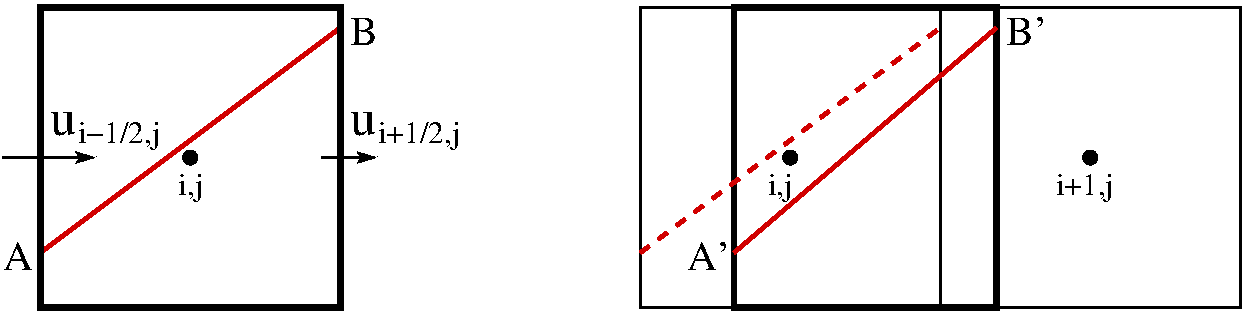
\includegraphics[width=0.75 \textwidth]{Figures/band1bis}
\end{center}
\caption{Advection of the AB interface segment. Face velocities at the left face, 
$u_{i-1/2,j} = -u_{1-}$, and the right face, $u_{i+1/2,j} = u_{1+}$,
are used to create an interpolated linear velocity field, so that point $A$ is advected 
to point $A'$ at the velocity $u_{i-1/2,j}$, point $B$ to $B'$ at  the velocity $u_{i+1/2,j}$, 
and a point along AB at a velocity linearly interpolated between $u_{i-1/2,j}$ and  $u_{i+1/2,j}$.}
\label{macfig}
\end{figure}
\begin{figure}
\begin{center}
    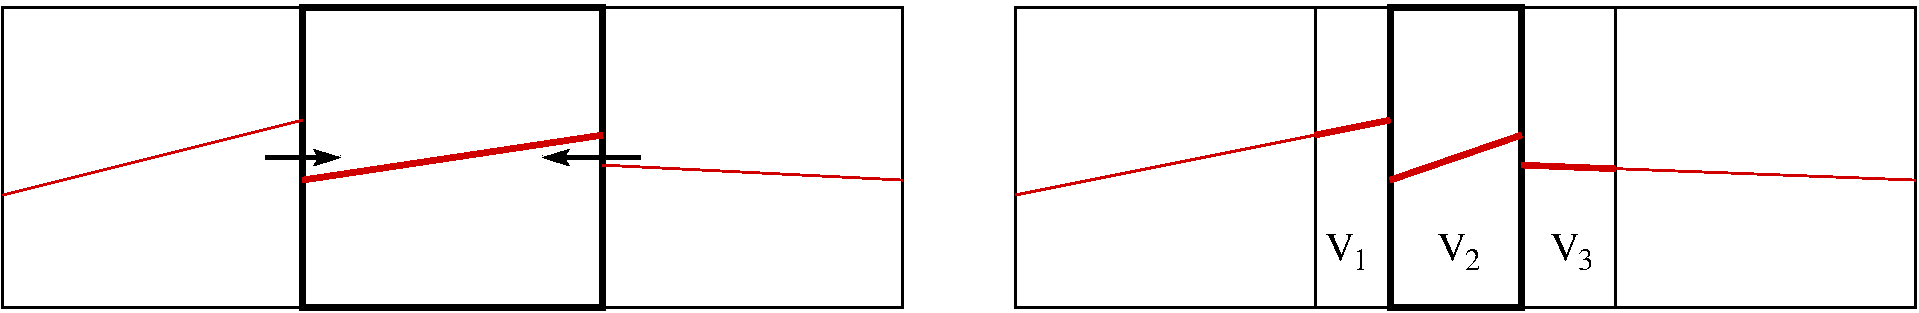
\includegraphics[width=\textwidth]{Figures/LE_mapping-horbis.pdf}
\end{center}
\caption{Formation of the volumes  $V_1,V_2$ and $V_3$ by Lagrangian advection in the $x$ direction. 
Left: initial reconstruction with the horizontal velocities on the faces of the central cell. 
Right: segments and volumes $V_i$ (see text) after Lagrangian advection (for simplicity it has been 
assumed $u_{i-3/2,j} = u_{i+3/2,j} = 0$)}
\label{lagfig}
\end{figure}
the color function is given by the sum of three contributions
\be
\cijk^{n,m+1} =  V_1 + V_2 + V_3 \,.
\nd
It is seen that the transform (\ref{map}) compresses distances by a factor 
$1 + \partial^h_m u_m = 1 + u_{m+} +  u_{m-}$. 
Thus the measure of any region of space is scaled by this amount under advection. 
The interface is then transfomed in three steps: 
1) compress all cells by the factor above; 
2) move the cells by $u_{m-}$; 
3) the moved cells now overlap the original cells. 
The volume corresponding to the overlap of the cell with itself is $V_2$, 
while $V_1$ and $V_3$ correspond
to the overlap with the moved cells from the left and right, respectively. 
The geometrical interpretation of the Lagrangian Explicit advection 
of Figs. \ref{macfig} and \ref{lagfig} and the definition
\eqref{faceint} of $F^{(c)}_{f}$ \blue{ leads to the following correspondence between 
the fluxes and the volume contributions $V_i$. 
To start with an example, for the central cell of Fig. \ref{lagfig} the flux on
the left face is from left to right, since $u_{1-} = - u_{i-1/2,j} < 0$.
This means that $V_1 =  - F^{(c)}_{1-,i} =  F^{(c)}_{1+,i-1} > 0$ while $V_3$ of the left cell, that
is $V_{3,i-1}$, is zero corresponding to an absence in that cell.
In all cases the fluxes accross a face are equal to the 
$V_1$ or $V_3$ of one cell or the other adjacent
to a face. }
The final expression of the split step is then
\be
\cijk^{n,m+1} =  \cijk^{n,m} (1  +  u_{m+} +  u_{m-} )  - F^{(c)}_{m-} - F^{(c)}_{m+} \,,
\label{sumflag}
\nd
which shows that the constant $c_m$ in the compression term is $\cijk^{n,m}$ while the 
approximation of the derivative is $\partial_m^h u_m =u_{m+}  + u_{m-} $ . 

It is interesting to note that using three Lagrangian advections in a sequence does not result in 
volume conservation to machine accuracy. Indeed the summation of the three substeps (\ref{sumf2}) 
results in 
\be
{\cijk^{n+1} - \cijk^{n}} = - \sum_{\rm{faces}\, f} F^{(c)}_f 
+ \sum_{m=1}^{3} \cijk^{n,m}(u_{m+}  + u_{m-}) \,.
\label{sumfall}
\nd
While the flux terms cancel upon integration over the domain, the sum of the compressive terms 
does not vanish since $\cijk^{n,m}$ changes during the three substeps.
We recover eq. \refeq{sumf2} with 
\be
c_m = \cijk^{n,m} \label{cmle}
\nd
\begin{figure}
\begin{center}
    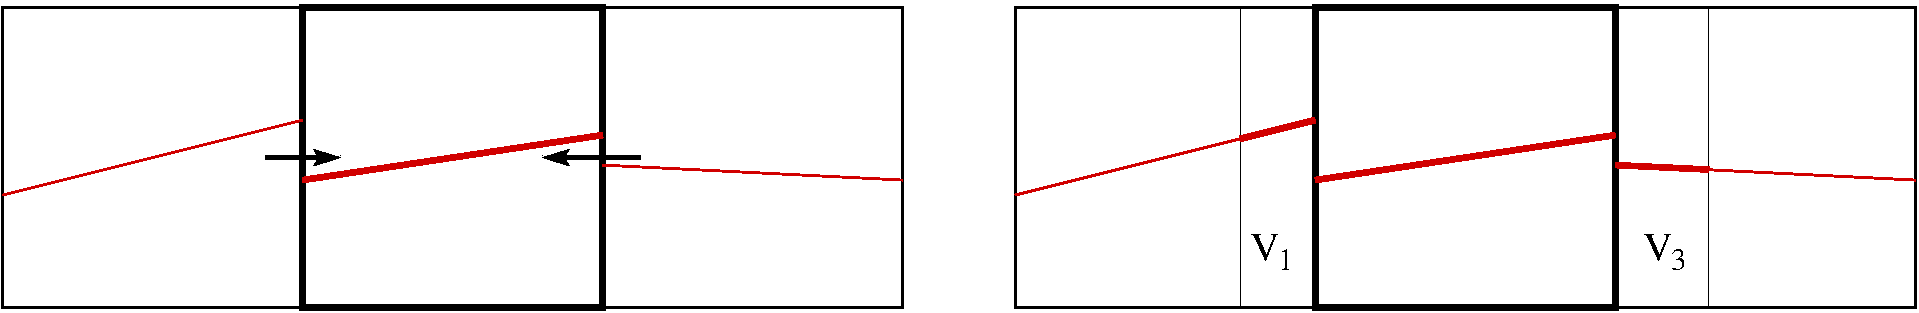
\includegraphics[width=\textwidth]{Figures/EI_mapping-horbis}
\end{center}
\caption{Eulerian flux representation for advection in the $x$ direction. 
Left: same initial reconstruction of Fig. \ref{lagfig} with the horizontal velocities 
on the faces of the central cell. 
Right: fluxes, or volumes $V_1$ and $V_3$, are calculated directly from the interface
reconstruction in each cell}
\label{eulflux}
\end{figure}

\subsubsection{Weymouth and Yue advection}

Another method that we shall describe is the exactly mass-conserving method of Weymouth and Yue (WY) 
described in ref. \cite{Weymouth:2010hy}. In that method the coefficient of the compression term  
(\ref{comp})
is independent of the direction $m$ so that $c_m = c$. The coefficient $c$ is defined as
\be
c=\Theta(\cijk^n - 1/2) \label{cmwy}
\nd
where $\Theta$ is the one-dimensional Heaviside function (defined on the real axis). 
That is $c=0$ if $\cijk^n < 1/2$ and $c=1$ if  $\cijk^n \ge 1/2$. 
The fluxes $F^{(c)}_f$ are also defined differently. The left fluxed volume in direction $m=1$ 
is equal to the volume fraction $F_{1-}^{(c)}$ in a cuboid of width $u_{i-1/2,j,k}$ 
(recall that $\tau = 1$) adjacent to the left face $f=1-$. This fluxed volume corresponds to 
``Eulerian Implicit'' (EI) advection in the terminology of \cite{Scardovelli02}
and is represented by the volume $V_1$ on Figure \ref{eulflux}. Using these definitions,  
Weymouth and Yue were able to show in ref. \cite{Weymouth:2010hy} that the final result obeys 
$C$-bracketing (see Section \ref{generalsplit}). 

Using  this advection method  results in volume conservation at machine accuracy. 
Indeed the summation of the three substeps (\ref{sumf2}) results in 
\be
{\cijk^{n+1} - \cijk^{n}} = - \sum_{\rm{faces}\, f} F^{(c)}_f 
+ c \sum_{m=1}^{3} \partial_{m}^h u_m \label{sumfall2}
\nd
Since $\sum_{m=1}^{3} \partial_{m}^h u_m = \sum_{m=1}^{3} (u_{m+}  + u_{m-}) $ is the simple 
finite-volume expression for $\nabla \cdot \U$, it disappears and mass is conserved at the 
accuracy with which condition (\ref{divu}) is satisfied. 

\subsubsection{Clipping}
\label{clipping}

The algorithm that has been coded involves a number of additional
steps designed to avoid unwanted effects of arithmetic floating point
round-off error. The most important one is clipping: at the end of
each directional advection, the values of $\cijk$ are reset so that
$C_{ijk}$ is set to $0$ is $C_{ijk} < \eps_c$ and $C_{ijk}$ is set to
$1$ is $C_{ijk} > 1 - \eps_c$. When there is no surface tension 
%with large curvature $\kappa h$ 
the choice $\eps_c = 10^{-12}$ works well.
Otherwise $\eps_c = 10^{-8}$ gives more stable results with smoother
interface shapes. This stronger clipping is a necessity for some
simulations with WY, while the CIAM method can survive $\eps_c =
10^{-12}$ with the diffusive interpolation schemes described below.  
As a matter of fact we observe that WY produces many more ``wisps'', 
i.e. cells with tiny values of $1-\cijk$
inside the liquid or $\cijk$ inside the gas.
We have not yet been able to determine the origin of this need for a more
forceful clipping with WY, but it could be related to the fact that the
CIAM method has a geometrical interpretation, while WY is intrisically algebraic
in nature.


\subsection{Momentum-advection methods}
\label{mom}

\newcommand{\dpt}[1]{\frac{\partial #1}{\partial t}}

\subsubsection{Advection of a generic conserved quantity}

Consider the advection of a generic {\em conserved} quantity $\phi$ by a continuous velocity field
\be
\dert \phi + \nabla \cdot ( \phi \U)  = 0. \label{phiconv}
\nd
We assume that $\phi$ is smoothly varying except on the interface where it may be discontinuous.
Indeed finding a correct scheme for the advection of this discontinuity, at the same speed as the advection of the 
volume fraction, is the goal of the present study.
The smoothness of the advected quantity away from the interface
is verified for the density $\rho$, the momentum $\rho \U$ or the internal energy 
$\rho e$. 
\newcommand\pijk{\phi_{i,j,k}}
Integrating the advection equation in time one obtains
\be
{\pijk^{n+1} - \pijk^{n}} = - \sum_{\rm{faces}\, f} F^{(\phi)}_f, \label{sumfp}
\nd
where the sum of the right-hand side is the sum over faces $f$ of cell $i,j,k$ 
of the fluxes $F^{(\phi)}_f$ of $\phi$. In equations, $F_f^{(\phi)}$ is defined in a similar manner to 
equation (\ref{faceint}) for the color function fluxes. 
\be
F_f^{(\phi)} = \int_{t_n}^{t_{n+1}} {\rm d}t \int_{f} u_f(\X,t) \phi(\X,t)  {\rm d}\X, \label{pfaceint}
\nd
where 
\be
u_f = \U\cdot \N_f, \label{uf}
\nd
 and $\N_f$ is the unit normal vector of face $f$, pointing outwards of cell $i,j,k$. 
In order to ``extract'' the discontinuity the flux can be expressed as
\be
F_f^{(\phi)} = 
\int_{t_n}^{t_{n+1}} {\rm d}t \int_{f} [ u_f  H \phi  +  u_f (1-H) \phi ]  {\rm d}\X , \label{fluxphi}
\nd
which can be re-expressed in terms of the fluxes $F^{(c)}$ in eq. (\ref{faceint}) as
\be
F_f^{(\phi)} = 
\bar \phi_1 \int_{t_n}^{t_{n+1}} {\rm d}t \int_{f} u_f H   {\rm d}\X + \bar \phi_2 \int_{t_n}^{t_{n+1}} {\rm d}t \int_{f}   
u_f (1-H) {\rm d}\X \label{barphi}
\nd
where 
\be 
\bar \phi_s = \frac{\int_{t_n}^{t_{n+1}} {\rm d}t \int_{f}  u_f  H_s \phi \, {\rm d}\X}{\int_{t_n}^{t_{n+1}} {\rm d}t \int_{f}  
u_f  H_s\,{\rm d}\X},  \label{barphi2}
\nd
and $H_1=H$, $H_2= 1-H$. This can be expressed as  
\be
F_f^{(\phi)} = \bar \phi_1 F_f^{(c)} +  \bar \phi_2 F_f^{(1-c)},
\nd
where $F_f^{(c)}$ is the flux of $H$ defined in (\ref{faceint}) and  $F_f^{(1-c)}$ is the flux 
obtained by replacing $H$ by $1-H$ in  (\ref{faceint}). 

\subsubsection{Cloning the tracers}

When a cell is cut by the interface, and the field $\phi$ is non-smooth, it becomes difficult to estimate
the integrals in (\ref{barphi}). A possibility is to define two new fields $\phi_{1,2}$ so that 
$\phi_s = \phi$ inside phase $s$. Then
\be
\phi = H \phi_1 + (1-H)\phi_2.
\nd
In the discretized equation, two discrete fields $\phi_{s,i,j,k}$ are defined over the entire domain $\Omega$.
This is more costly in memory usage but simplifies considerably the computation of the averages in Equation
 (\ref{barphi}). The two equations (\ref{phiconv}) and (\ref{interfadv}) are now replaced by three equations,
the same volume fraction equation  (\ref{interfadv}) and the two equations
\bea
\dert \phi_1 + \nabla \cdot ( \phi_1 \U)  &= 0&  \label{pcv1}, \\ 
\dert \phi_2 + \nabla \cdot ( \phi_2 \U)  &= 0& \label{pcv2} . 
\nda
The three equations (\ref{interfadv},\ref{pcv1}-\ref{pcv2}) now imply (\ref{phiconv}). This addition of a pair of ``cloned'' variables to help deal with large variations of density is similar to the methods used for the resolution of the momentum and energy equations for compressible flow. For example Saurel and Abgrall used two density, momentum and energy variables in ref. \cite{Saurel99}, leading to their seven-equations model, while Allaire, Clerc and Kokh use two density variables in \cite{allaire02}, leading to their five-equations model. The addition of a cloned tracer variable in incompressible isothermal flow was also implemented by Popinet in the ``Basilisk'' code \cite{basilisk}. 

\subsubsection{Advection of the density field}

Let us now apply the above considerations to the advection of the density
field by a general continuous velocity field.
Although in the incompressible case the density follows trivially the color
function, it will allow us to introduce an important point
about the equivalence of tracer and VOF advection. 
The density $\rho(\X,t)$ obeys eq. (\ref{phiconv}) with 
$\phi = \rho$. %There is no compression term in eq. (\ref{phiconv}). 
The advection of density may be made consistent with the advection of the color function by 
using fluxes  $F_f^{(c)}$ and estimating
the average occuring in equation (\ref{barphi2}),  
$\bar \phi_1 = \bar \rho$ from averages over control volumes or approximations on faces.

The case relevant here is that of an incompressible velocity field, with uniform density in each phase. 
Then $\rho$ is exactly proportional to $H$ (Eq. \ref{muH}).
The constancy of $\rho$ allows to extract it trivially from the integrals in eq. (\ref{barphi}) 
and to obtain {\em exactly} $\bar \rho_s = \rho_s$. 
Then the flux of $\rho$ is  
\be
F_f^{(\rho)} = \rho_1 F_f^{(c)} +  \rho_2 F_f^{(1-c)}.\label{fluxrho}
\nd
Using this flux definition for $\rho$, and any VOF method for the fluxes of the color function, 
one obtains a conservative method for $\rho$ since eq. (\ref{sumfp}) 
evolves $\rho$ as a difference of fluxes. 
That is, one conserves the total mass and 
$\sum_{i,j,k} \rho^{(n)}_{i,j,k} =  \sum_{i,j,k} \rho^{(n+1)}_{i,j,k}$. 
However this result is not consistent with the advection of the color function in the CIAM case, 
since as we have seen above, CIAM does not conserve volumes exactly, 
that is $\sum_{i,j,k} C^{(n)}_{i,j,k} =  \sum_{i,j,k} C^{(n+1)}_{i,j,k}$ is not in general true. 
As a result the advection of $\rho$ 
is not consistent with the advection of $C$. 

The paradox may be resolved if one notices that the compression term is missing 
in the equation for the advection of $\rho$. 
One should keep the compression term, which is not changing the equation 
in the case of incompressible velocity fields, so that the equation 
for the conserved quantity $\phi$ or $\rho$ becomes
\be
\dert \phi + \nabla \cdot ( \phi \U)  = \phi \, \nabla \cdot \U \label{phiconv2}
\nd
It is then possible to define the evolution of $\rho = \phi$ through a sequence of 
directionally split operations exactly equivalent to the operations performed on the color function. 
\be
{\pijk^{n,m+1} - \pijk^{n,m}} = - F^{(\phi)}_{m-} - F^{(\phi)}_{m+} 
+ (\tilde \phi_1^m c^{(1)}_m + \tilde \phi_2^m c^{(2)}_m ) \partial_{m}^h u_m \label{sumfpconsistent}
\nd
where $F^{(\phi)}_{m\pm}$ is defined as above, and
\be
\tilde \phi_s^m = \frac{\int_{t_n}^{t_{n+1}} {\rm d}t \int_{\Omega}  \phi  H_s  \partial_{m}^h u_m  \,  {\rm d}\X}
{\int_{t_n}^{t_{n+1}} {\rm d}t \int_{\Omega} H_s  \partial_{m}^h u_m \,{\rm d}\X}
\nd
 and 
where $c^{(1)}_m=c_m$ is the compression coefficient computed as in the VOF advection from $\cijk^{n,m}$
and $c^{(2)}_m= 1 -c_m$ corresponds to the symmetric color fraction  $1 - \cijk^{n,m}$.
Specifically for $\rho$ this gives 
\newcommand\rijk{\rho_{i,j,k}}\be
{\rijk^{n,m+1} - \rijk^{n,m}} = - F^{(\rho)}_{m-} - F^{(\rho)}_{m+} + C_m^{(\rho)},\label{sumfrho}
\nd
where the fluxes are given by (\ref{fluxrho}) 
and the central compression part is
\be
C_m^{(\rho)} =  (\rho_1 c^{(1)}_m + \rho_2 c^{(2)}_m ) \partial_{m}^h u_m  \label{central}
\nd
with no implicit summation on $m$. The $c_m^{(s)}$ values are given by (\ref{cmle}) or
(\ref{cmwy}). 
It is interesting to note that for the WY method, the compression terms 
eventually cancel and mass is conserved at the same accuracy as the discrete incompressibility condition
$\partial_{m}^h u_m=0$ is verified. 

\subsubsection{Momentum advection: basic expressions}

Momentum advection can be performed following the general outline above. 
Each momentum component 
can be treated by considering the transport of the conserved quantity  
$\phi=\rho u_q$ where $q$ is the component index. 
Reworking equations (\ref{fluxphi},\ref{barphi}) and (\ref{barphi2}), with this
definition, we obtain for the weighted averages 
$\bar \phi_s = \overline { \rho u_q}_s$ in phase $s$ the expression
\be 
\overline{\rho u_q}_s = \rho_s \bar u_{q,s} 
\nd
where 
\be \bar u_{q,s} =  \frac{\int_{t_n}^{t_{n+1}} {\rm d}t \int_{f}  u_q u_f  H_s  \, {\rm d}\X}{\int_{t_n}^{t_{n+1}} {\rm d}t \int_{f}  u_f  H_s\,{\rm d}\X} \label{barudef}
\nd
We term $\bar u_{q,s}$ the ``advected interpolated velocity'' and 
we will explain below how these ``advected'' velocities are computed. 
Thus the evolution of the momentum is given by
\newcommand\mijk{(\rho_{i,j,k} u_{q;i,j,k})}
\begin{eqnarray}
{\mijk^{n,m+1} - \mijk^{n,m}} & = &  \nonumber \\
- F^{(\rho u)}_{m-} - F^{(\rho u)}_{m+}
 + ( \rho_1 \tilde u_{q,1}^m  c^{(1)}_m &+ & \rho_2 \tilde u_{q,2}^m c^{(2)}_m ) \partial_{m}^h u_m 
\label{sumfrou}
\end{eqnarray}
where
\be
 F^{(\rho u)}_{f} =  \rho_1 \bar u_{q,1}  F^{(c)}_{f}  +  \rho_2 \bar u_{q,2}  F^{(1-c)}_{f},
\nd
and the ``central interpolated velocity'' corresponding to the $\tilde \phi_s$ are
\be
\tilde u_{q,s}^{m} = \frac{\int_{t_n}^{t_{n+1}} {\rm d}t \int_{\Omega} u_q^{n,p}  H_s  \partial_{m}^h u_m   \,  
{\rm d}\X}
{\int_{t_n}^{t_{n+1}} {\rm d}t \int_{\Omega}   H_s  \partial_{m}^h u_m \,{\rm d}\X} \label{tildeudef}
\nd
where for CIAM  $p=m$ and for WY  $p=1$. Thus $\tilde u_{q,s}^{m}=\tilde u_{q,s}$ remains constant while the various
steps $m=1,..,3$ of directional splitting are performed. Note that we otherwise omit the superscript $m$ 
for $\bar u_q$ and $\tilde u_q$ to avoid too complex notations. 
Notice that ``cloning'' the advected velocities 
$\bar u_{q,1}$ and $\bar u_{q,2}$
would make it easier to advect a velocity field with a jump on the interface. 
However in viscous flow without phase change the velocity is continuous on the 
interface, and to avoid an excessively complicated method we 
approximate the velocity field 
as continuous and we choose approximations of the ``advected interpolated velocity'' such that
$\bar u_q =  \bar u_{q,1} = \bar u_{q,2}$ and ``central interpolated  velocity'' such that $\tilde u_q =  \tilde u_{q,1} = \tilde u_{q,2}$. 
An important simplification is then 
\be
 F^{(\rho u)}_{f} = \bar u_q F^{(\rho)}_{f} \label{frou}
\nd
(which is the central equation in this development) and thus
\be
{\mijk^{n,m+1} - \mijk^{n,m}} =  -\bar u_q  F^{(\rho)}_{m-} - \bar u_q  F^{(\rho)}_{m+} 
+ \tilde u_q^m C_m^{(\rho)},\label{sumfmom2}
\nd
where the density fluxes are defined in (\ref{fluxrho}) and the central term $C^{(\rho)}$ is defined
in (\ref{central}). 
In the above expression the weighted average velocities $\bar u_q$ are computed 
using (\ref{barudef}) on the corresponding
left face $m-$ or right face $m+$. 

The scheme above must be combined with an advection scheme for the
color fraction. When the CIAM scheme is used, the $C_m^{(\rho)}$ term in (\ref{sumfmom2})
must be kept to ensure consistency with VOF advection. This term is computed using 
the above definition (\ref{cmle}). 
This term does not cancel when the final momentum is computed 
from the three directionally-split advections and the result is not exactly conservative. 
 On the other hand when the WY scheme is used the
$c^{(s)}_m$ and $\tilde u_q^m$ factors are independent of $m$ and 
\be
C_m^{(\rho)} =  [\rho_1 c + \rho_2 (1-c )] \partial_{m}^h u_m  \label{central2}
\nd
so provided the velocity field is incompressible (that is $\sum_{m=1}^3 \partial_{m}^h u_m =0$)
summing the three split advection expressions (\ref{sumfmom2}) one obtains a cancellation of the central terms and 
\be
{\mijk^{n,4} - \mijk^{n}} =  - \sum_{\rm faces \, f}  \bar u_{q,f}  F^{(\rho)}_{f} . \label{sumfmomtotfracstep}
\nd
The version of our method coupled with WY advection is thus exactly conservative. 
Both CIAM and WY  methods can be rewritten in a slightly different notation useful for future discussion
\be
{\hat g_q^{n+1} - g_q^{n}} =  - \sum_{\rm faces \, f}  \bar u_{q,f}  F^{(\rho)}_{f}(C^n,u_f)
+ \sum_{m=1}^3 \tilde u_q^m C_m^{(\rho)},\label{advect-ed-ing}
\nd
where $\hat g_q^{n+1}= \mijk^{n,4}$ is the $q$-component of the final momentum, $g_q^{n}= \mijk^{n}$ 
is the initial one,
and we have written explicitly the dependence of  $F^{(\rho)}_{f}(C^n,u_f)$ on the face velocities
and on the volume fraction field in the neighborhood of the interface. 

\subsubsection{Momentum advection: interpolations and flux limiters}

The evolution of momentum as expressed in eq. (\ref{advect-ed-ing})
can be approximated either
 1) away from the interface, in the bulk of the phases or
 2) in the neighborhood of the interface.
In the first case the expression simplifies considerably since the density  as well as the color fraction
are constant thus $\rho_{ijk} = \rho_0$ and $C^n = C_0$. The spurious central term is also removed so
\be
{u^{*}_q - u_q^{n}} =  - \sum_{\rm faces \, f}  \bar u_{q,f} u_f . \label{sumfmomtot}
\nd
We can distinguish an ``advecting'' velocity $u_{f}$ and an ``advected velocity component'' 
$\bar u_{q,f}$ which must be estimated in an integral relating to face $f$.
Both components are either centered on the face of the staggered set of cells / control volumes for the
component $u_q$ or estimated close to the face $f$. 
 Typical hyperbolic equation methods use interpolants to perform these estimations. 
The interpolants we use here are one-dimensional and work from the node velocities on a segment aligned
with the direction of advection, that is the direction perpendicular to face $f$. 
Thus the scheme in the bulk is 
\be
{u^{*}_q - u_q^{n}} =  - \sum_{\rm faces \, f}  \bar u_{q,f}^{\rm (advected)} u^{\rm (advecting)}_f . \label{sumfmomtotbulk}\nd
Near the interface we have instead
\be
{\hat g_q^{n+1} - g_q^{n}} =  - \sum_{\rm faces \, f}  \bar u_{q,f}^{\rm (advected)}  F^{(\rho)}_{f}(C^n,u_f^{\rm (advecting)})
+ \sum_{m=1}^3 \tilde u_q^m C_m^{(\rho)},\label{advect-ed-ing-2}
\nd
To estimate the advecting velocities $u_f^{\rm (advecting)}$ we use centered schemes. 
(see Figure \ref{stag-grid} for a visual depiction of the arrangement of the staggered nodes.)
Consider for example that the face is perpendicular to direction $1$ so 
 $f=1_\pm$.
There are two cases. In the first case the advected component is not aligned with the 
face normal so in the example $q\neq 1$.   Consider specifically the case $q=2$ depicted in 
Figure \ref{stag-grid}(b). The
staggered $u_2$ control volumes are centered on $i,j+1/2,k$. The face $f=1_\pm$ is then 
centered on $i-1/2,j+1/2,k$.
Then  $u_f^{\rm (advecting)} = u_{1_-}^{\rm (advecting)} =   u_{1;i-1/2,j+1/2,k}$ which is not given and has to be interpolated by
\be
 u_{1;i-1/2,j+1/2,k}^{\rm (advecting)} = \frac12(  u_{1;i-1/2,j,k} +  u_{1;i-1/2,j+1,k}).
\nd
In the second case the advected component is aligned with the 
face normal  so in the example $q= 1$ also depicted in 
Figure \ref{stag-grid}(a).
The staggered $u_1$ control volumes are centered on $i+1/2,j,k$. The face $f=1_\pm$ is then 
centered on $i-1,j,k$ and the interpolation is
\be
 u_{1;i-1,j,k}^{\rm (advecting)} = \frac12(  u_{1;i-1/2,j,k} +  u_{1;i+1/2,j,k}).
\nd
 
Now we turn to the definition of the {\em advected} velocity values $u_{q,f}$ in expression
(\ref{advect-ed-ing-2}).
We still take the example where  the face is perpendicular to direction $1$ so 
 $f=1_\pm$ (we take the case $f=1_-$ to illustrate, see Figure \ref{advect-ed-ing-fig}(a)) thus the {\em advecting} direction is $x_1$. 
We only need to consider the
dependence of the advected velocity on $x_1$ to define the interpolation. 
We consider the regularly spaced one-dimensional grid of advected velocities. In order to use lighter
notations we will note $\phi = u_q$ the {\em advected} velocity component, with known node values at
\be
\phi_p = u_q (x_{1,1_-} + p h )
\nd
where $x_{1,1_-}$ is the coordinate of the face  $f=1_-$. 
The  known values $\phi_p$ in the staggered grid are at nodes that
are a half-integer away from the face, which implies that the known values
are 
\be
u_{1;i-3/2,j,k} =  \phi_{-3/2},\quad u_{1;i-1/2,j,k} = \phi_{-1/2},\quad   u_{1;i-1/2,j,k} = \phi_{1/2}, \cdots
\nd
when $q=1$,  $x_{1,1_-} = ih$  and
\be
u_{2;i-2,j+1/2,k} =  \phi_{-3/2},\quad  u_{2;i-1,j+1/2,k} = \phi_{-1/2}, \quad  u_{2;i,j+1/2,k} = \phi_{1/2}, \cdots
\nd
when $q=2$. For $q=2$ or 3, we have  $x_{1,1_-} = (i-1/2)h$ so the $q=3$ case follows easily.
We need to predict
$\phi_0$ to serve as an approximation of $\bar u_q$ given in (\ref{barudef}) . 
An interpolation function is now defined that predicts 
this value as a function of the four nearest points,
and in an upwind manner based on the sign of the {\em advecting} velocity $u_f$, 
given by centered interpolations. 
The value at the face is given by 
\be
\phi_0 = f(\phi_{-3/2}, \phi_{-1/2}, \phi_{1/2},\phi_{3/2},{\rm sign}(u_f)) \label{simpleinterp}
\nd
\red{
In this study we have extensively tested two kinds of interpolations or schemes
\begin{enumerate}
\item A scheme that uses a QUICK third order interpolant in the bulk, away from the interface and a simple first order upwind flux near the interface. We call this scheme QUICK-UW.
\item A scheme that uses a Superbee slope limiter \cite{roe1985some}. for the flux in the bulk and a more complex Superbee limiter tuned to a shifted interpolation point near the interface.  We call naturally call this scheme ``Superbee''. 
\end{enumerate}
We describe each scheme in turn, starting with the QUICK-UW. For 
positive advecting velocity and in the bulk we have
% inter(x0,x1,x2,x,y0,y1,y2)
%
%    if (u(i-1,j,k)+u(i,j,k)>0.0) then
%      work(i,j,k,1) = inter(xh(i-1),xh(i),xh(i-2),x(i),u(i-1,j,k),u(i,j,k),u(i-2,j,k))  !
%                                                             y0        y1          y2
%                                                             φ-1/2    φ1/2      φ-3/2
%                                               !  inter = 0.75*y0 +0.375*y1 -0.125*y2
\be
\phi_0 = \frac 3 4   \phi_{-1/2} + \frac 3 8   \phi_{1/2} - \frac 1 8 \phi_{-3/2}
\nd
while near the interface $\phi_0 = \phi_{-1/2}$. 
For negative (to the left) advecting velocity and in the bulk we have
\be
\phi_0 = \frac 3 4   \phi_{1/2} + \frac 3 8   \phi_{-1/2} - \frac 1 8 \phi_{3/2}
\nd
while near the interface $\phi_0 = \phi_{1/2}$ (see also \cite{Tryggvason11}))
In the Superbee case, we start by defining a general family of interpolants that can be expressed as}
\be
f(\phi_{-3/2}, \phi_{-1/2}, \phi_{1/2},\phi_{3/2},{\rm sign}(u_f)) = \phi_{-1/2} + S h/{2} 
\nd
for a positive advecting velocity % $u_f > 0$.
where the slope $S$ is given  by a slope-limiter function $g$ such that
$S= g(\phi_{-3/2}, \phi_{-1/2}, \phi_{1/2})$
while for a negative advecting velocity % $u_f<0$
\be
f(\phi_{-3/2}, \phi_{-1/2}, \phi_{1/2},\phi_{3/2},{\rm sign}(u_f)) = \phi_{1/2} - S h/{2} 
\nd
where $s= g(\phi_{-1/2}, \phi_{1/2},\phi_{3/2})$.

To define the slope $S$ used in Superbee consider the factor $\alpha$ to be
the smallest in absolute value of
\begin{eqnarray}
\alpha^+=(\phi_{1/2,j} -\phi_{-1/2,j})/ h ,  \nonumber \\
\alpha^-=2 (\phi_{-1/2,j} -\phi_{-3/2,j})/ h . 
\end{eqnarray}
and the factor $\beta$ to be the smallest in absolute value of 
\begin{eqnarray}
\beta^+=2 (\phi_{1/2,j} -\phi_{-1/2,j})/ h ,  \nonumber \\
\beta^-=(\phi_{-1/2,j} -\phi_{-3/2,j})/ h . 
\end{eqnarray}
Then one prescribes $S$ as the largest, in absolute value, of $\alpha$ and  $\beta$.
\begin{figure}
\begin{center}
    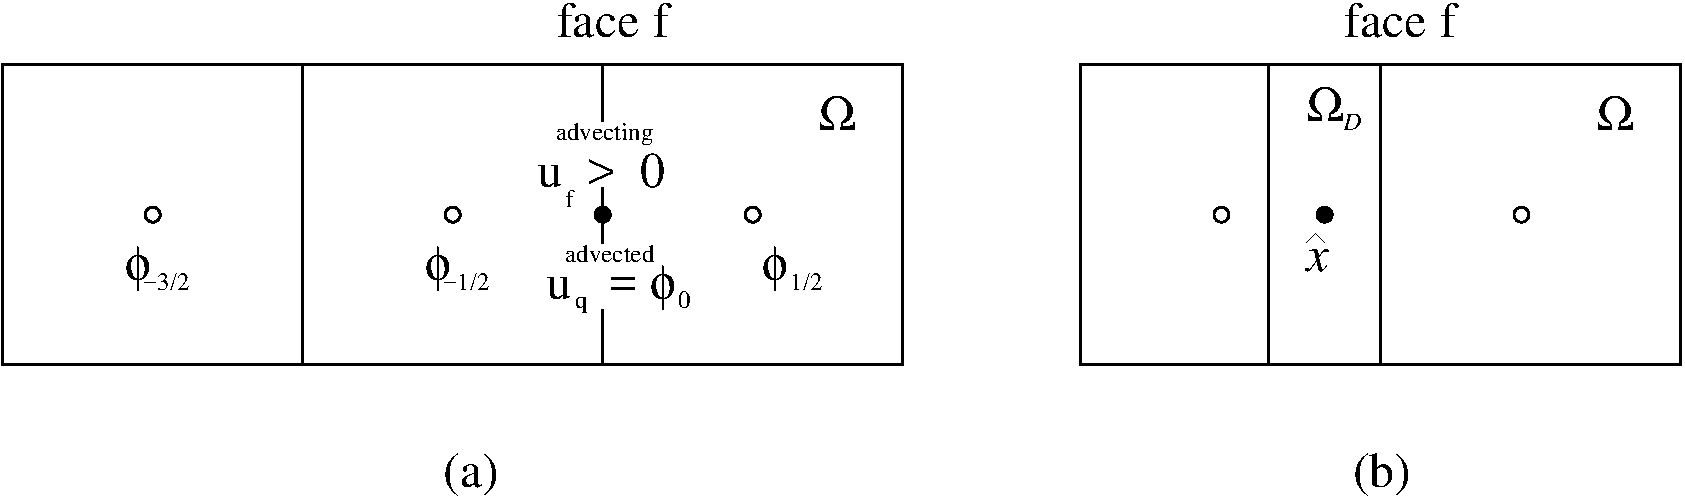
\includegraphics[width=\textwidth]{Figures/advect-ed-ing.pdf}
\end{center}
\caption{(a) The advected and advecting velocities in expression (\ref{advect-ed-ing-2}) 
  are both located on or near face $f$ (in this case $f=1-$). The reference control volume
$\Omega$ for the advected velocity component $u_q$ is also shown. The arrangement is the same
whatever the component $q$ but here the example of a horizontal advection ( case $f=1-$ ) is taken. 
The value of the advected velocity component $\bar u_q = \phi_0$ on the center of 
face $f$ (full disk) is interpolated (see text) from the values $\phi_{p}$ of $u_{q}$ on the nodes (open disks). 
(b) A more sophisticated interpolation predicts the value $\phi(\hat x)$ where $\hat x$ is
at the center of the ``donating'' region $\Omega_D$ (see text).}
\label{advect-ed-ing-fig}
\end{figure}
%\subsubsection{Momentum advection: tuned interpolations near the interface}
\label{tunedinter}

A slightly different estimate of the Superbee advected velocity is used near the interface. First we extend 
the definition of the interpolants as we shall predict $\bar u_q$ at a point $\hat x$ 
slightly upwind from $x_f$ using a new function $\hat f$ so that
\be
\phi_0 = \hat f(\hat x,\phi_{-3/2}, \phi_{-1/2}, \phi_{1/2},\phi_{3/2},{\rm sign}(u_f)). \label{mp}
\nd
We take  $\hat x = x_f - u_f \tau/2$ to be the midpoint of the fluxed region. (This is the region from which
flow lines crossing the face originate see Figure \ref{advect-ed-ing-fig}(b).)
The extended interpolant is defined for positive velocity %  $u_f>0$ 
as
\be
\hat f(\hat x,\phi_{-3/2}, \phi_{-1/2}, \phi_{1/2},\phi_{3/2},{\rm sign}(u_f)) = \phi_{-1/2} +  S |\hat x - x_{-1/2}|
\nd
and for negative velocity % $u_f<0$ 
as
\be
\hat f(\hat x,\phi_{-3/2}, \phi_{-1/2}, \phi_{1/2},\phi_{3/2},{\rm sign}(u_f)) = \phi_{1/2} -  S |\hat x - x_{1/2}|
\nd
The rationale behind this choice is as follows. For a time-independent advecting velocity field $u(\X,t)$, 
the integrals in expression
(\ref{barudef}) can be simplified
\be
\phi_0 = \bar u_q = \frac{\int_{\Omega_D}  u_f u_q \, {\rm d}\X}{ \int_{\Omega_D}  
u_f  \,{\rm d}\X}.  \label{barphi3}
\nd
where ${\Omega_D} $ is the ``donating region'' (see \cite{Tryggvason11})  from which
flow lines crossing the face originate. Then
since we approximate the advecting velocity $u_f$ by its midpoint value  the integral
can be further simplified as
\be 
\bar u_q = \frac 1{|\Omega_D|} \int_{\Omega_D}  u_q \, {\rm d}\X  \label{barphi4}
\nd
Since the ``midpoint'' at $\hat x$ is the center of mass of the donating region ${\Omega_D}$ 
the interpolation expression (\ref{mp}) follows. 

\subsubsection{VOF-consistent Momentum advection: staggered grids.}

In order to apply the above method on the staggered grid, 
the fluxes and control volumes of the momentum must be in
correspondence with the fluxes and control volumes of the VOF color
function.  This is realized by recreating in each velocity control
volume the necessary color fraction data. 

At the start of the velocity advection operations summarized by the operator 
$\LLL^h_{\rm conv}$ each velocity control volume say $\Omega_{i+1,j,k}$ overlaps two VOF control volumes
$\Omega_{i,j,k}$ and $\Omega_{i+1,j,k}$ ( see figure \ref{halffractions}) 
The following operations are performed:

\begin{enumerate}
\item Reconstruction of the volume fractions and density $C^{n}$ and $\rho^{n}$ in the staggered control volumes 
$\Omega_{i+1/2,j,k}$ corresponding to the momentum component $\rho u_1$, thus obtaining the ``half fractions'' $\tilde C^{n}$ and  $\tilde \rho^{n}$. 
\item Computation of the initial momentum component $\tilde g_1^{n} = \tilde \rho^{n} u_1^{n}$.
\item Split advection of the momentum in the $x$ direction 
using the method in the previous sections to obtain 
the first component of the new momentum $\hat g_1^{n+1}$.
\item Split advection in the $x$ direction of the volume fractions and density in the staggered control volumes 
using the volume of fluid method to obtain predicted densities $\hat\rho^{n+1,1}$.
\item Repeat the previous split advection operations for momentum and density in $y$ and $z$. At each time step, the sequence $x, y, z$
is permuted. Eventually one obtains $\hat g_1^{n+1}$ and $\hat\rho^{n+1}$.
\item Repeat the previous operations for the two other momentum components $g_2$ and  $g_3$. 
\item Extraction of the  new velocities components $\U^{*}=\hat \G^{n+1}/\hat\rho^{n+1}$.
\item In parallel, computation of $C^{n+1}$ from $C^n$ on the centered cells using
the VOF method. 

\end{enumerate}

We now cover the eight steps in detail. 
The reconstruction of the volume fractions in the staggered cells (step 1) implies considering each control volume for a velocity component, say $\Omega_1=\Omega_{i+1/2,j,k}$ for the $u_1$ component, and finding the ``half'' volume fraction
in each intersection $ \Omega_{i+1/2,j,k} \cap  \Omega_{i,j,k}$ and  $ \Omega_{i+1/2,j,k} \cap  \Omega_{i+1,j,k}$ 
(see Figure \ref{halffractions}). The ``half-fractions'' are found using the reconstruction parameters
$\alpha$, $\M$ in equation (\ref{mxalpha}) in the original
centered control volume, and then computing the corresponding volume fractions in the half 
cells. Addition of the two half fractions leads to an estimate of the volume fraction $\tilde C^n_{i+1/2,j,k}$ in the staggered cells, and thus of the densities $\tilde \rho^n_{i+1/2,j,k}$. 

In step 2, now that the staggered cell densities at the beginning of the time step are known, 
obtain the momentum component $g^n_{1,i+1/2,j,k} = \rho^{n}_{i+1/2,j,k} u^{n}_{1,i+1/2,j,k}$. 
This momentum component can be advected (step 3) using the method described in the previous section, to 
obtain  $\hat g^{n+1}_{1,i+1/2,j,k}$  in a  conservative manner
following equation (\ref{advect-ed-ing}). 
Similarly the  volume fractions in the staggered cells are also reconstructed and advected in
direction $x_1$  in step 4. 
Then in step 5 the other directionally split advections are performed. 
After each direction, the newly obtained densities and advected velocities are used for the next direction
but the advecting velocities remain the same. The central velocity stepping is discussed 
below equation (\ref{tildeudef}) above. 
Finally the advections are performed in each of the three systems of staggered cells (step 6) to obtain  
$\hat C^{n+1}_{i+1/2,j,k} = \hat C^{n,4}_{i+1/2,j,k}$  where the 
notation $C^{n,m}$ was introduced in equation (\ref{sumf2}) and $m$ indicates which direction of the 
split time step was performed. Then $\hat \rho^{n+1}_{i+1/2,j,k} = \rho_1 \hat  C_{i+1/2,j,k} + \rho_2 ( 1 - \hat C_{i+1/2,j,k} ) $ obtains.
Finally the $\LLL_{\rm conv}$ operator is obtained as (step 7) 
\be
 \LLL_{\rm conv} =  \frac 1 \tau (\hat \G^{n+1} - \tilde \rho^{n} \U^n \label{unp11})
\nd
where as above we use the $\tilde \rho$ notation to indicate that the density has been 
reconstructed in the staggered cells.
In the absence of the other operators in $\LLL_2$ this would result 
in
\be
\U^* = \hat \G^{n+1}/ \hat \rho^{n+1}.
\nd
However (leaving aside the pressure and other contributions in equation  (\ref{fotm}))
 the momentum on the staggered cells at the beginning of the next
time step is not equal to the momentum $\hat \rho^{n+1} \U^{n+1}$ at the end of the previous 
time step but is rather defined as $\tilde \rho^{n+1} \U^{n+1}$ where  $\tilde \rho^{n+1}$ is 
obtained at beginning of the time step from the half-fractions. That is, $C^{n+1}$ is computed 
directly from $C^{n}$ on the centered cells (step 8) and this allows to find 
 $\tilde C^{n+1}$ and from it, $\tilde \rho^{n+1}$ , by running again step 1. These densities  $\tilde \rho^{n+1}$ are not
the same as the  $\hat \rho^{n+1}$  densities of the previous time step. This implies non conservation of the momentum.
We note that  attempting to always use only the three sets
 $C^{n}_{i+1/2,j,k}$,  $C^{n}_{i,j+1/2,k}$,  $C^{n}_{i,j,k+1/2}$ and evolve them by 
the VOF method on the staggered cells 
would maintain conservation but result in the three staggered grids evolving independently of each other and
eventually diverging.
\begin{figure}
\begin{center}
    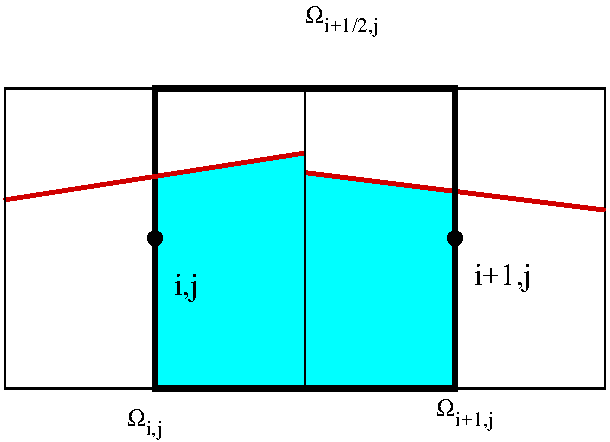
\includegraphics[width=0.5\textwidth]{Figures/halffractions.pdf}
\end{center}
\caption{Computation of the staggered fractions from the half-fractions}
\label{halffractions}
\end{figure}
\clearpage

\subsection{Description of the other time-split terms}

The other time-split terms in equation (\ref{conspredictedvel}) and in the projection
step (\ref{fotm}) are solved in a standard centered way. The density on the faces
of the central cells $\Omega_{i,j,k}$ is estimated using a centered average
$\rho_{i+1/2,j,k} = (\rho_{i+1/2,j,k} + \rho_{i+1/2,j,k})/2$. Although this is less accurate and consistent
than the usage of the half fractions $\hat \rho_{i+1/2,j,k}$ described above the average 
is used in these terms both for simplicity reasons and because tests have shown the usage
of $\hat \rho_{i+1/2,j,k}$ to lead to less stable simulations than the centered average. 

The velocities in the diffusion term are introduced in an explicit way. Although this requires small
time steps of the order $\rho h^2/\mu$ the capillary restriction on time steps
is usually even smaller, being of order $\tau = (\rho h^3/\sigma)^{1/2}$. The two restrictions
become of the same order when $h \sim l_{\mu \sigma}$ where $l_{\mu \sigma} = \mu^2 / (\sigma \rho)$ 
is the length at which the viscous and capillary terms balance. For water, this length is 
of the order of 10 nanometers, and grids of that size are not used in the flows we consider. 
However, should the velocities be treated in an implicit manner, we do not believe this would
change the conclusions of this paper. 

Surface tension is computed using the Continuous Surface Force method proposed by 
\cite{brackbill92}, together with an estimate of the curvature through the computation
of height functions, in a manner that closely follows the method of \cite{popinet09}. 
The external forces in equation (\ref{conspredictedvel}) 
are only gravity and are computed in a trivial manner with 
$\frac 1 {\rho^{n+1}} \LLL_{ext} =  \G$, where gravity $\G$  is a constant. 





\section{Testing and Validation}
\label{test}
\subsection{Consistent cylinder advection}

An elementary test of our method, that mostly verifies that the coding 
has been performed correctly, considers a uniform planar velocity field 
$u_1 = u_2 = 1.6 \times 10^{-2}$ and a droplet of density $\rho_l = 10^9$ 
in gas at density $\rho_g=1$ with a CFL number of $0.0256 \sqrt 2$.  
Viscosity and surface tension are set to zero in this test.  
The diameter of the droplet is $D/h=3.2$. The unit domain is discretized on a 
$16 \times 16$ grid. The droplet shapes that result are shown on the left 
of Figure \ref{CylAdv}. 
The irregularities seen in the advected droplet are due to the roughness of 
the VOF approximation at such low resolutions. We repeat the test with 
conditions close to air/water: viscosity $\mu_l = 0.1$, $\mu_g=0.002$ 
and  $\rho_g=1$, $\rho_l = 10^3$ with identical results: a viscosity contrast 
will not generate numerical instabilities on a uniform velocity field, as shown 
on the right of Figure~\ref{CylAdv}. 
% ----------------------------------------
\begin{figure}
\centering
\begin{minipage}{0.48\textwidth}
\centering
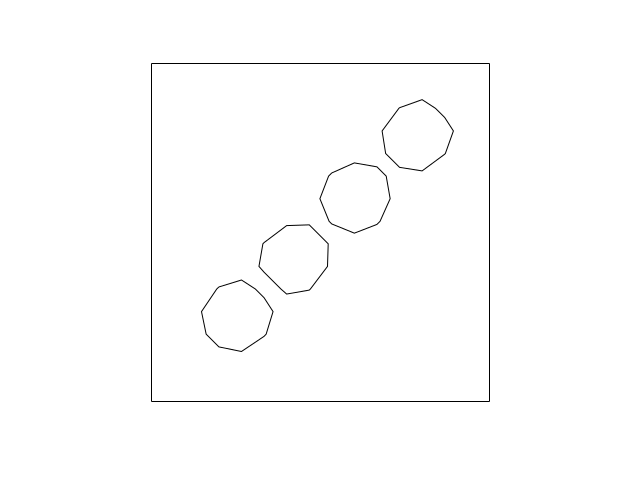
\includegraphics[width=0.98\textwidth]{Figures/cylinderadvection.png}
\end{minipage}
% ---
\begin{minipage}{0.48\textwidth}
\centering
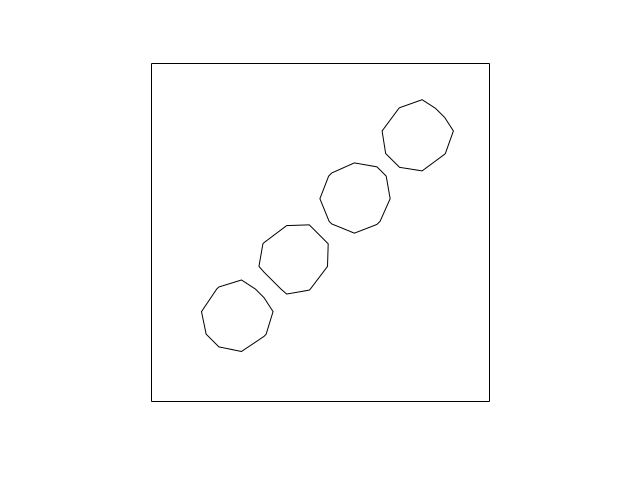
\includegraphics[width=0.98\textwidth]{Figures/cylinderadvectionviscous.png}
\end{minipage}
\caption{Large-density-ratio droplet in a uniform velocity field: a droplet 
with $D/h=3.2$ grid points per diameter is advected in 3D in the plane $z=0$ 
(see text); left:  density ratio $10^9$ without viscosity,
right: density ratio $10^3$ with viscosity}
\label{CylAdv}
\end{figure}
% ----------------------------------------

\subsection{Kelvin Helmholtz Instability}

The Kelvin-Helmholtz instability arises between unequal velocity fluid
streams. It is closely related to the issues addressed in the current
paper since it arises in many of the flows for which the current
method is designed, such as atomisation. Moreover, the
Kelvin-Helmholtz instability is particularly strong on a vortex sheet,
since (as we show below) it has for an infinitely thin sheet a
divergent growth rate as the wavenumber goes to infinity. Compounding
the issue, the baroclinic term of the vorticity equation leads to the
creation of a vortex sheet. In previous papers some of us have studied the
Kelvin-Helmholtz instability in viscous flows with surface tension
\cite{yecko02,boeck05,bague10}

We focus in this paper on the inviscid, no surface tension case since the
objective is to assess the manner in which the advection terms are
treated numerically. Moroever the inviscid, no surface tension case is
a kind of ``worst-case scenario'' without the stabilizing effects of viscosity
and capillarity.

The simplest setup is that of vortex sheeet, for which the growth rate is
given by
\be
\om_i = \frac{2 \sqrt r}{r+1}  k U  \label{omkazi}
\nd




\subsection{Sudden acceleration of a cylinder at large density contrast}

A test that is often included in studies of momentum-conserving methods
\cite{bussmann2002modeling,desjardins10,raessi12,le13,Vaudor:2017ip}
and other methods designed to improve the stability of two-phase flow
computations \cite{Fuster2013energy} is to initialize a droplet of very
high density at velocity $\U_l(\X)=U_0 \E_x$ with the other lighter fluid at
rest, so that $\U_g(\X)=0$. Surface tension and viscosity are not present 
as in the previous test, the only difference being the
discontinuity of the initial velocity on the interface. 
The initial velocity condition amounts to a vortex sheet on the surface 
of the cylinder. After the first time step, the projection method (\ref{fotm}) 
adds a dipole potential flow so that $\U_g = U_0 \E_x + \tau \nabla p / \rho_g$ 
in the gas around the droplet, identical to the dipole flow around a solid object.
However in addition to the dipole flow there could be small multipole components 
to the outer gas flow. 
There are three ways to estimate the perturbations created on the interface.
% ----------------------------------------
\begin{figure}
\begin{center}
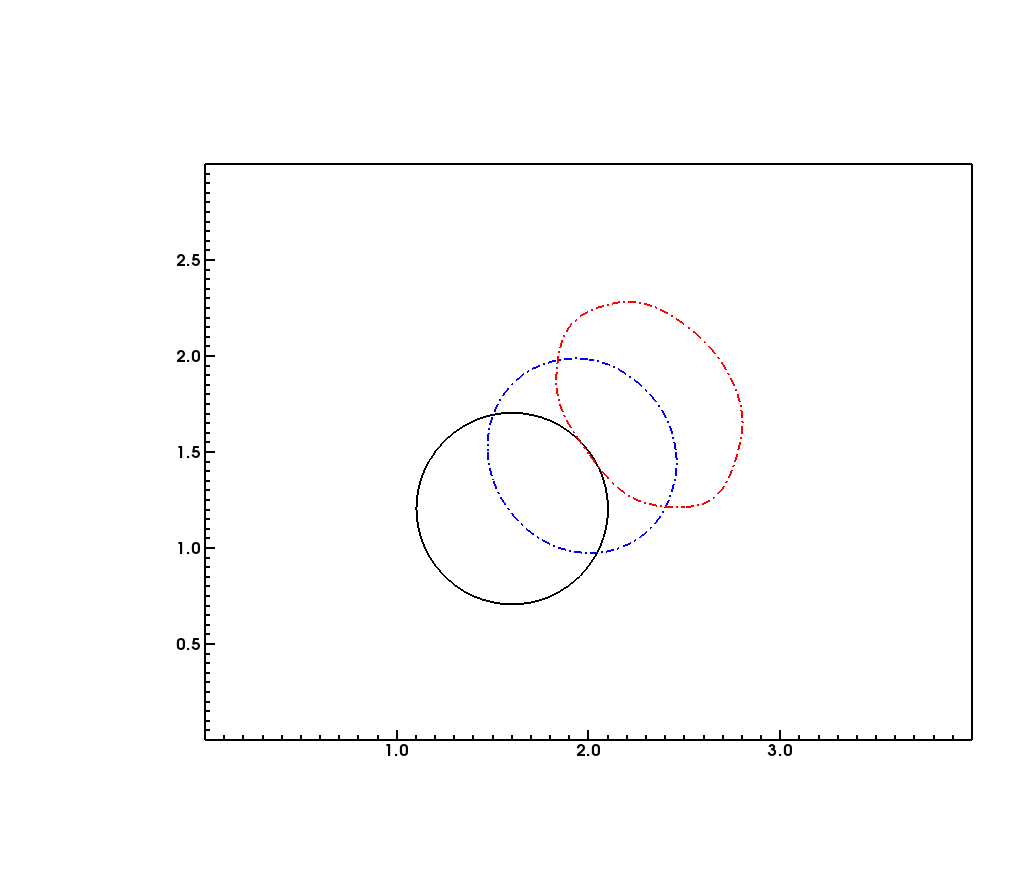
\includegraphics[width=0.4\textwidth]{Figures/Sagar/a.png}
\quad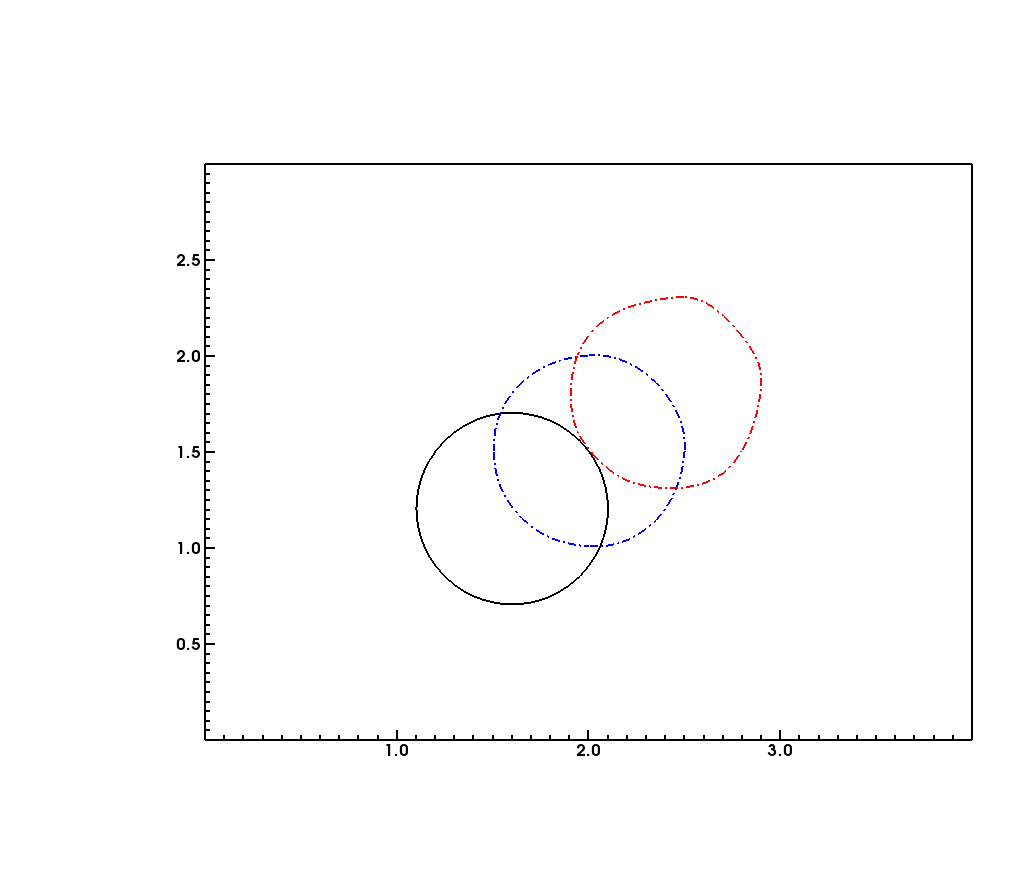
\includegraphics[width=0.4\textwidth]{Figures/Sagar/b.png} \\
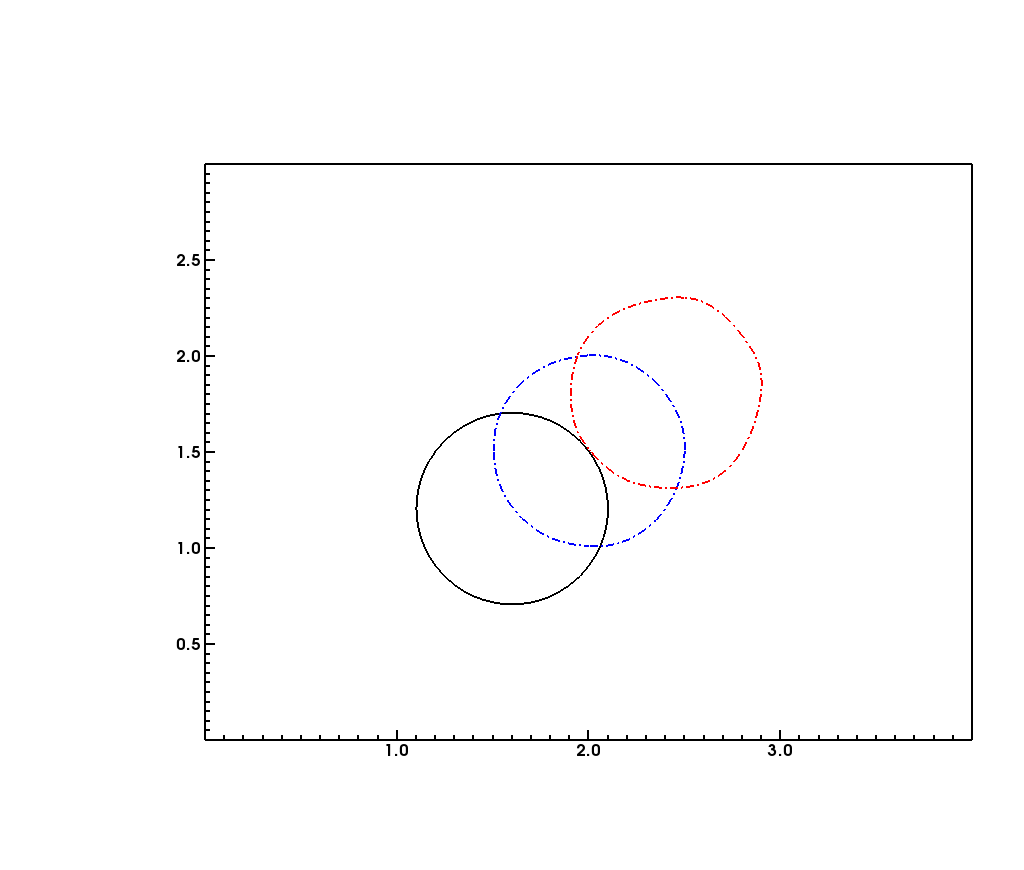
\includegraphics[width=0.4\textwidth]{Figures/Sagar/c.png}
\quad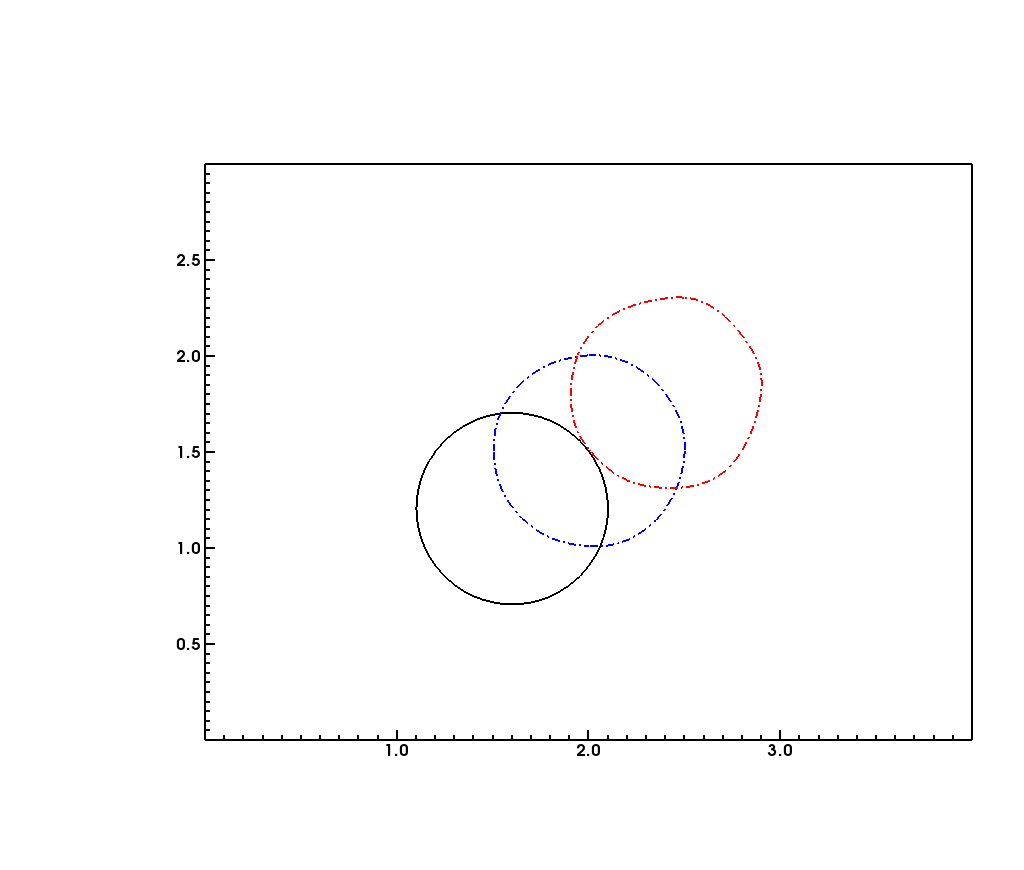
\includegraphics[width=0.4\textwidth]{Figures/Sagar/d.png} \\
\end{center}
\caption{Deformation of a droplet moving through a light fluid. 
From left to right and top to bottom: $r=10,10^3,10^6,10^9$. 
Black shape at $t=0$, blue at $t=D/(2U)$ and red at $t=D/U$. 
The grid resolution is $D/h=20$.}
\label{rich}
\end{figure}
% ----------------------------------------

% ----------------------------------------
\begin{figure}
\begin{center}
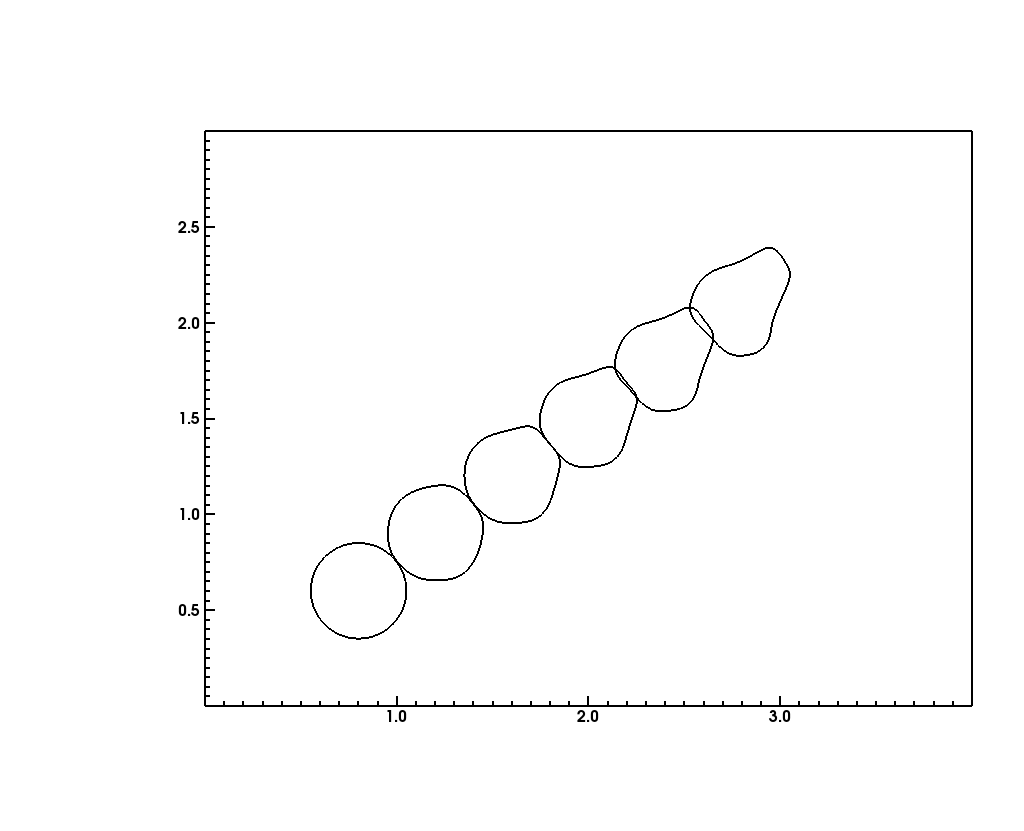
\includegraphics[width=0.4\textwidth]{Figures/Sagar/long.png}
\end{center}
\caption{Deformation of a droplet moving through a light fluid at $r=10^9$.
The grid resolution is $D/h=20$.}
\label{long}
\end{figure}
% ----------------------------------------
A vortex sheet is unstable with respect to the Kelvin-Helmholtz instability. 
The main results about the amplitude of the instability are as follows. 
Let $A(t)$ be the maximum deviation of the interface which has a dimension of length. 
For flows with no viscosity and surface tension
as is the case here, the  Kelvin-Helmholtz instability amplitude $A(t)$  should grow exponentially from a perturbation 
of wavenumber $k$ as $A(t) \sim A(0) \exp ( s_k t )$ with $s_k =| \Delta U | k/ \sqrt r  $ where $ \Delta U $ is
the tangential velocity difference and $r=\rho_l/\rho_g$. In the limit of large $r$ the growth rate becomes small. Since the maximum wavenumber on the grid is $\pi/h$ an estimate of the growth rate of the small wavelength instabilities is $\pi U_0 N/(D \sqrt r)$ where $N$ is the number of grid points per diameter. After advection by a droplet diameter, the 
elapsed time is $\Delta t = D/U_0$. For typical values in the literature of $r=10^6$ and an arbitrary value of 
$N=32$ the amplitude growth would be 
\be
\exp (s_{\rm max} \Delta t) =  \exp\left( \frac{\pi N}{ \sqrt r} \right) 
= \exp ( 0.032\pi) = 1.1058\ldots
\nd
which means the amplitude should grow by 10\% after advection by one diameter 
and by $e^{1/2}$ after the typical advection by 5 diameters. 

Beyond the linear growth stage of the Kelvin-Helmholtz instability, there is a 
self-similar, non-linear growth stage for which dimensional analysis implies
that $A(t) \sim | \Delta U | t/ \sqrt r $ \cite{hoepffner11}. By this argument 
also the perturbation of the cylinder should remain  of order  
$A(\Delta t) \sim D / \sqrt r$ after advection by a droplet diameter. 
One should note that the self-similar growth is obtained for vanishing boundary 
layer thickness but we precisely expect such a velocity discontinuity in 
the present case with no viscosity. 

A final, physical deformation is expected from the spatial pressure variation 
induced by the dipole gas flow. This variation involves a larger pressure at 
the aft and fore stagnation points and a lower pressure along the ``equator'' 
of the droplet \cite{Clift78}. The resulting integrated stress is of order 
$\rho_g U^2$ resulting in the growth of the droplet deformation as 
$A(t) \sim U^2 t^2 / (D r)$ and after advection by a droplet diameter as
$A(\Delta t) \sim D / r$. 
This growth is observed experimentally \cite{opfer14} and results in an 
elliptically shaped drop, albeit of much smaller amplitude than the two former 
Kelvin-Helmholtz-related growth mechanisms. 

The results are shown on Figure \ref{rich} for several times and
density ratios in a manner comparable to \cite{bussmann2002modeling}. For these
numerical experiments, the exact manner of initializing the velocity fields has 
some importance. It is important not to allow in the first time step some gas 
velocity in the liquid to avoid large pressure gradients in the liquid. 
Thus the density is initialized to $\rho_l$ to machine accuracy using the 
{\sc Vofi} library \cite{bna2015numerical,bna2016vofi}
within a disk implicitly defined by $x^2 + y^2 + z^2 < R^2$ 
and the velocity is initialized to 1 for all the velocity nodes inside
a disk implicitly defined  by  $x^2 + y^2 + z^2 < (R+nh)^2$, where $n$ is the 
size of the ``halo'' in number of grid points. The velocity in the other
nodes is initialized to 0. The tests shown were performed with $n=1$. 
Increasing the size of the halo from $n=0$ to $n=1$ improves the results in the 
first phase of the droplet motion, but not in the late phase. 

The velocity of the motion has been oriented on the diagonal as in 
\cite{bussmann2002modeling}. The WY scheme is used with a QUICK
interpolant. The droplet deforms little after advection by one droplet 
diameter (Figure \ref{rich}). For longer advection the deformation is worse 
but, as explained above, this is to be expected
at high resolution, except in the $r=10^9$ case for which we show advection 
by 5 diameters in Figure \ref{long}. 
If the non-momentum-conserving method is used, the
droplet deforms rapidly and the simulation breaks down. As expected
the results are better than those of \cite{Fuster2013energy}, that uses the
skew-symmetric scheme but without momentum-conserving-like schemes, 
but worse than those of \cite{bussmann2002modeling,desjardins10,raessi12,le13}. 
It is also seen, as expected from the developments above, 
but perhaps contrary to intuition, that it is easier
to have larger density contrasts. Increasing the number of grid points also helps.


A comment can be made on the nature of the instabilities seen. If
 the gas velocity numerically diffuses inside the liquid, then some vorticity
may penetrate into the liquid despite the fact that in inviscid flow
vorticity should remain confined on the interface. If this happens,
the growth rate of a single-phase Kelvin-Helmholtz instability inside the 
liquid is the much larger value $\widetilde{s}_k =| \Delta U | k/2$, 
without the $\sqrt r$ factor at denominator. \red{(The derivation of this fact 
may be found for example in \cite{matas2011experimental}.)} 
The instability seen for the $r=10^9$ case for the long advection case in  Figure \ref{long} is 
a mode 3, which excludes the large linear growth discussed above for small 
wavelenghts rather points to the velocity diffusion mechanism. 
Minimizing numerical diffusion should then be an important
quality for this test, while on the other hand numerical diffusion may
stabilize other difficult test cases/situations. 

\red{
\subsection{Sheared layer}
In order to better analyze the behavior of the methods in flow under shear, 
such as vortex sheets and Kelvin Helmholtz instabilities, we setup directly 
a planar, parallel shear flow in a $(-1/2,1/2)^2$ domain with the following 
initial condition
\bea
u_1& = 15 &\qquad {\rm if \;\;} |x_2| > 1/10 \nonumber \\
u_1& = 1  &\qquad {\rm if \;\;} |x_2| < 1/10 \nonumber 
\nda
$$
u_2  =  0.01\, \sin(2 \pi x_1) \exp(-20 x_2^2)
$$
and $\rho=1$  if $|x_2| > 1/10$ and $\rho=10^3$ otherwise. 
This flow is similar to a liquid sheet in high velocity gas. The flow is 
simulated until time $t_f=2$ unless the simulation blows up at an earlier time
$t_b <t_f$.
Table \ref{shearmtable} shows the numerical schemes that have been used in a few
simulations together with the fraction $t_{b}/t_f$ of the final time that has 
been reached. All simulations have been performed on a $128\times128$ grid with 
a CFL of 0.03 and a density ratio of 1000. The new method (MC) is
systematically more stable than the standard method for the two combinations 
shown in Table \ref{shearmtable}: a) the WY VOF scheme and the QUICK-UW velocity 
interpolation schemes and b) the CIAM VOF with the Superbee slope limiters. 
The state of the two simulations with the first combination of schemes is shown
in Figure~\ref{shelay}, just before breakdown at time $t_b = 0.34$ 
(or $t_b/t_f = 0.17$) for the (MC) method, and at time  $t_b = 0.16$ 
(or $t_b/t_f = 0.08$) for the standard method. We have also tested a number of other
combinations, for example  WY \& Superbee that turns out to be very unstable.  
We have also performed simulations with smaller  $64\times64$ and $32\times32$ 
grids that yield similar results. 
Finally, we note that this case is also unstable in a single-phase configuration 
when using the QUICK third-order velocity interpolation.
% -----
\begin{table}
\input notes
\caption{Percentage of completion of the shear layer test with various methods. 
All simulations are performed on a $128\times128$ grid with a CFL of 0.03 
and a density ratio of 1000.}
\label{shearmtable}
\end{table}
% -----

% -----
\begin{figure}
\begin{center}
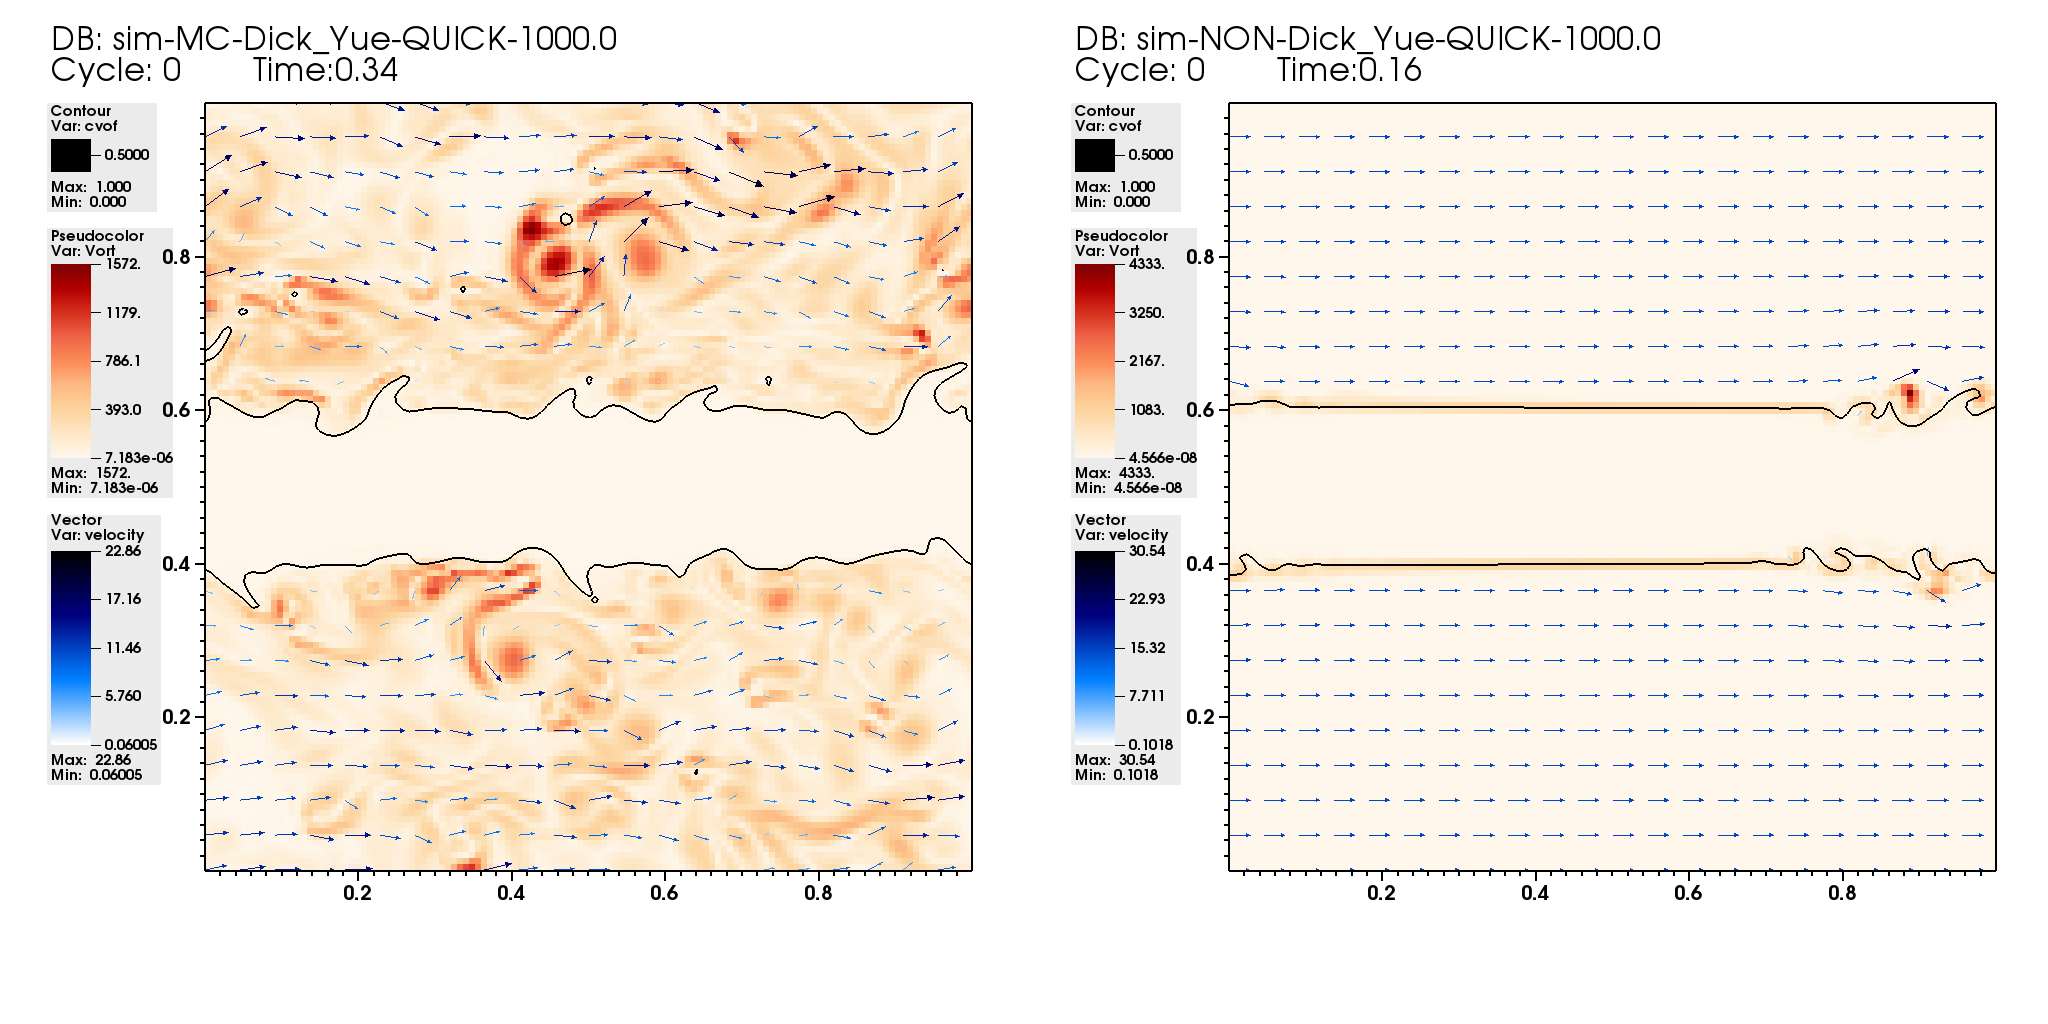
\includegraphics[width=\textwidth]{Figures/Sagar/shear.png}
\end{center}
\caption{The state of the simulation of the sheared layer just before eventual 
breakdown of the simulation with the combination of WY VOF scheme
and QUICK-UW interpolation. Left: (MC) method, right: standard method.}
\label{shelay}
\end{figure}
% -----
} 
% end red section

\subsection{Falling Raindrop}
% Basic setup 

A flow configuration that combines the complexities of high density-ratios with the interaction between capillary, viscous and inertial stresses is that of a water droplet falling in air under the influence of gravitational acceleration. The problem is characterized by a combination of Reynolds, Weber and Bond numbers, the definitions of which are as follows : 

\begin{align}
We=\frac{\rho_{\rm air} U^2 d}{\sigma} \quad,\quad Re= \frac{\rho_{\rm air} U d}{\mu_{\rm air}} \quad,\quad Bo=\frac{\left(\rho_{\rm water}-\rho_{\rm air}\right) g d^2 }{\sigma}
\end{align}

\vspace*{0.2cm}

In our particular numerical setup, $We \simeq 3.2 $, $Re \simeq 1455 $ and $Bo \simeq 1.0 $, thus corresponding to that of a $3mm$ diameter raindrop (a relatively large one) falling in air at an approximate terminal velocity of  $8$ m/s (interpolated from empirical data, refer to  \cite{gunn1949terminal}). The parameters in the problem setup is given in Table \ref{raindropprop}, and the schematic diagram given by Fig. \ref{setup}. The droplet is initially placed at the center of a cubic domain (3D), whose side is 4 times the diameter of the drop. 

\vspace*{0.2cm}

% -----
\begin{table}[h!]
\begin{center}
\begin{tabular}{ccccccc}
\hline\hline
$\rho_{\rm air}$ & $\rho_{\rm water}$ & $\mu_{\rm air}$ 
& $\mu_{\rm water}$ & $\sigma$ & $d$ & $g$\\
$\left(kg/m^3\right)$ & $\left(kg/m^3\right)$ & $\left(Pa \, s\right)$ 
& $\left(Pa \,s \right)$ & $\left(N/m\right)$ & $(m)$ & $(m /s^{2})$ \\
\hline
1.2 & $0.9982 \times 10^3$ & $1.98 \times 10^{-5}$ & 
$8.9 \times 10^{-4}$ & $0.0728$ & $3 \times 10^{-3}$ & $9.81$\\
\hline\hline
\end{tabular}
\caption{Parameter values used in the simulation of a falling water droplet in air. \label{raindropprop}}
\end{center}
\end{table}
% -----

\vspace*{0.2cm}

In order to properly reproduce and analyse the dynamics of a relatively large drop (high Reynolds flow) such as in our case, the numerical method has to accurately resolve the thin, complicated boundary layers, the interaction of such layers with the capillary deformations and finally the non-linear feedback of the complex 3D vortical structures in the droplet wake to the surrounding pressure field. Therefore, we explicitly state that the aim of this particular test case is not to develop a high fidelity model of a raindrop, but rather carry out a stringent evaluation of the robustness of our numerical method compared to methods which are not momentum consistent. For such a low Weber number the capillary forces dominate and the droplet should remain approximately spherical, and should definitely not undergoe any subsequent atomization. 


% -----
\begin{figure}[h!]
\begin{center}
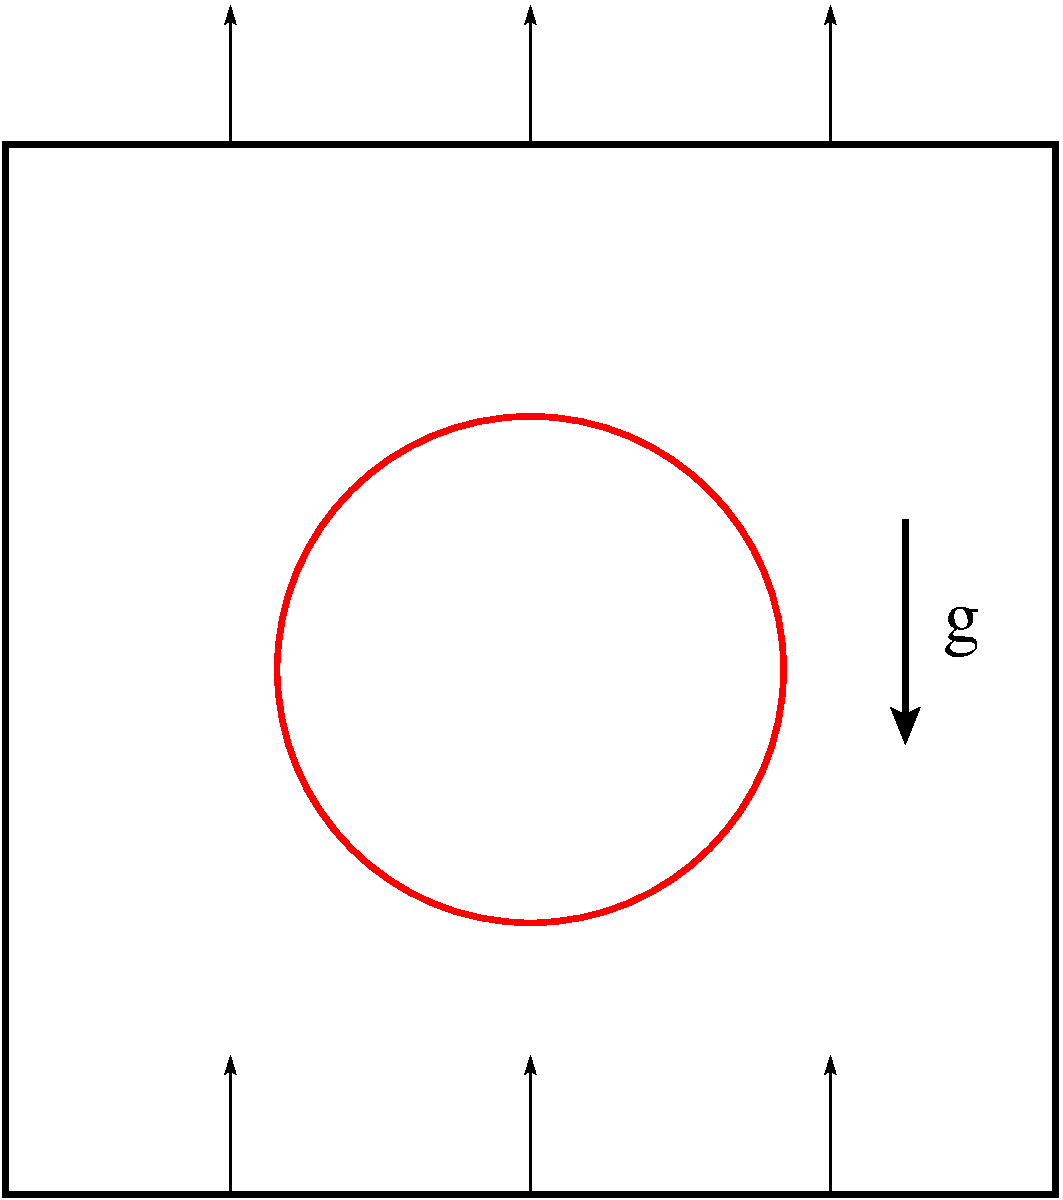
\includegraphics[width=0.35\textwidth]{Figures/setup.pdf}
\end{center}
\caption{Problem setup for falling rain drop test case. Boundary conditions 
at the top and bottom are a uniform inflow and outflow velocity $U_0(t)$. 
Boundary conditions on the side are free slip (no shear stress).}
\label{setup}
\end{figure}
% -----


% -----
\begin{figure}
\begin{center}
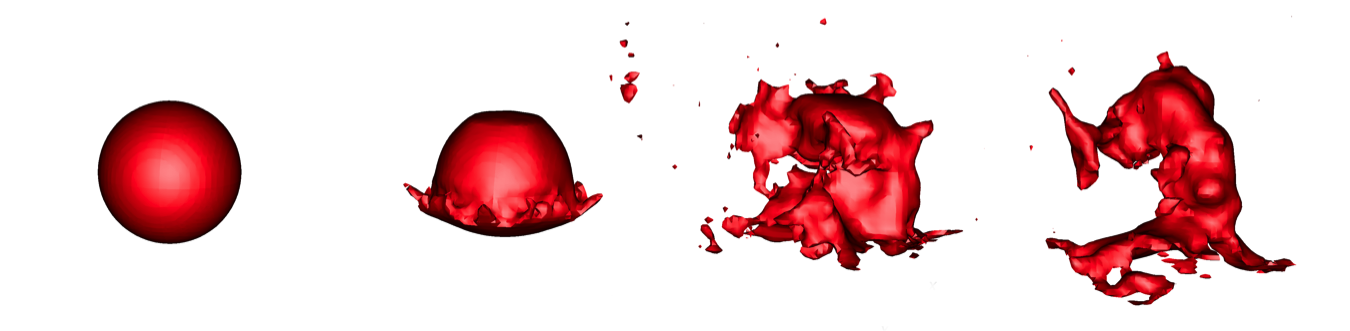
\includegraphics[width=0.75\textwidth]{Figures/cata.png}
\end{center}
\caption{Rain drop test case: catastrophic breakup with non-conserving 
formulation, $D/h=30$.}
\label{cata}
\end{figure}
% -----

Numerical simulations of this test case at moderate resolution ($D/h=16$ to 64 grid points per diameter were tested) without the consistent momentum-conserving scheme described in this paper, results in the catastrophic deformations of the droplet as shown in Fig. \ref{cata}, which we like to describe as 'fictitious' or 'artificial' atomization as a result of rapidly growing numerical instabilities. This effect was previously uncovered by \cite{Xiao:2014vs} in a similar case involcing the sudden interaction of a droplet at rest with a uniform gas flow. The Weber number in that case was also approximately 3, therefore one would expect a nearly spherical droplet shape, but the authors of ref. \cite{Xiao:2014vs} have reported a similar catastrophic deformation, forwarding the following explanation. To start with, we neglect gravity and viscous effects at this relatively large Reynolds number. Also, we are interested in steady-state flow. On the axis and near the hyperbolic stagnation point at the front of the droplet one has $u_2=0$ for the transverse (radial) velocity and for the axial momentum balance

\be
u_1 \partial_1 u_1 = - \frac 1 \rho \partial_1 p.
\nd

Because of the low viscosity and large density ratio, it is not possible for the air flow to immediately entrain the water, so the fluid velocity is significantly smaller in the water. In the air the acceleration near the stagnation point is of the order $U^2/D$, whereas the pressure gradient is

\be
\partial_1 p \sim \rho_{a} U^2/D.
\nd
The pressure gradient in the water is much smaller, however in the case of a mixed cell the water density multiplies the air acceleration $U^2/D$, so that
\be
\partial_1 p \sim \rho_{w} U^2/D,
\nd

then a large pressure gradient results in the mixed cell or cells. This large pressure gradient results in a large pressure inside the droplet near the front stagnation point, as shown in Figure \ref{FengXiao}. This large pressure is balanced by surface tension only for a sufficiently large curvature near the droplet front. This explains the presence of a ``dimple'' often observed in low resolution simulations of the falling drop. 

% -----
\begin{figure}
\begin{center}
\begin{tabular}{cc}
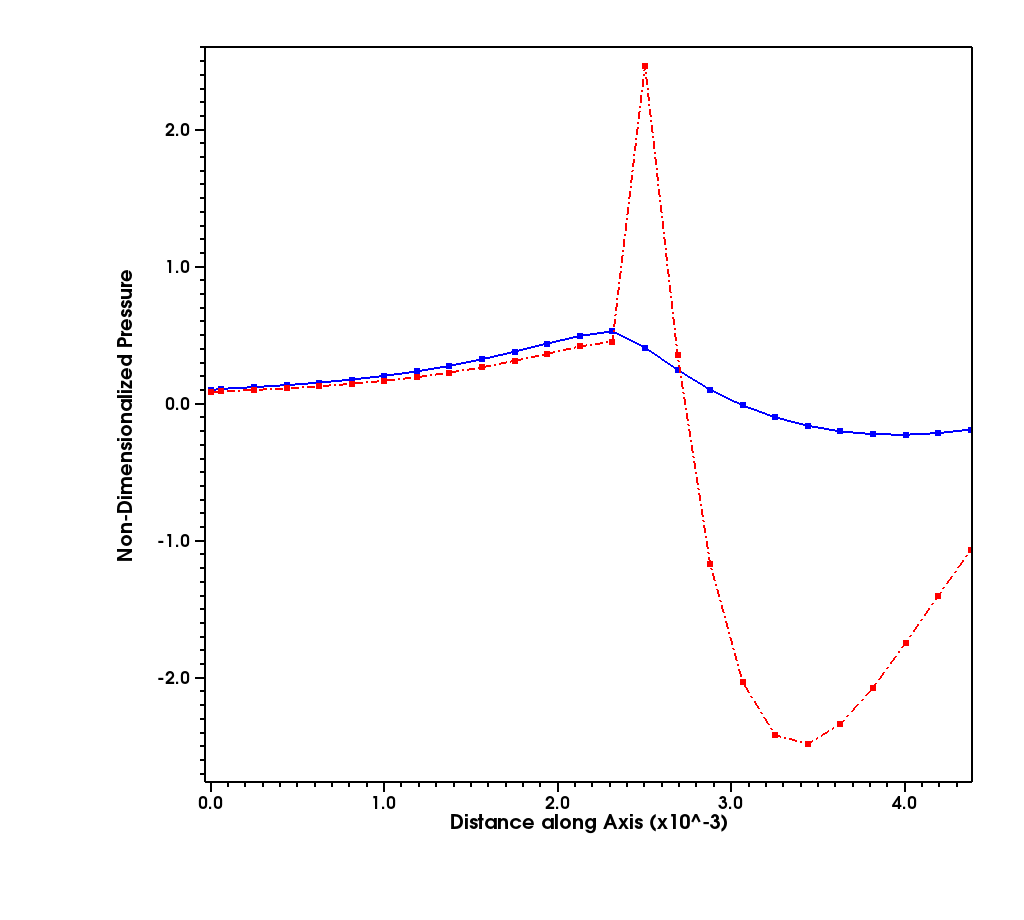
\includegraphics[width=0.45\textwidth]{Figures/Sagar/16ppd_MC_vc_NON-MC.png} &
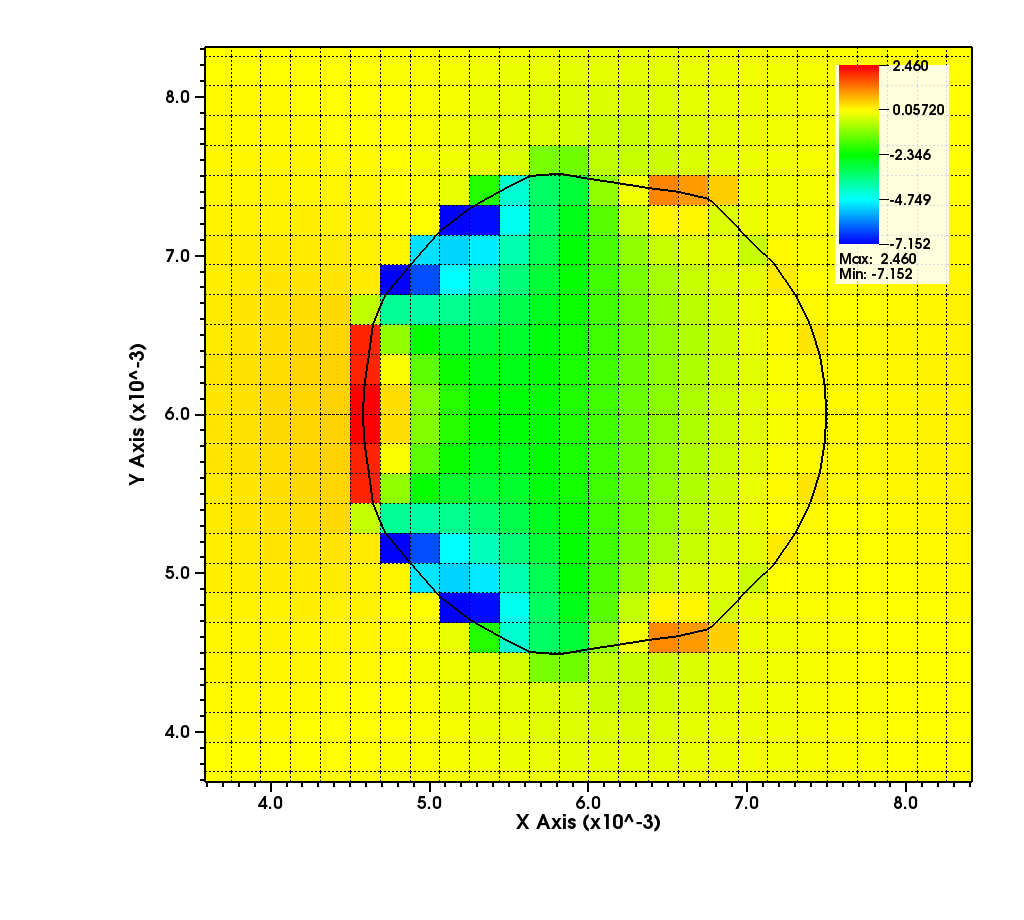
\includegraphics[width=0.45\textwidth]
{Figures/Sagar/non_MC_16ppd_pressure_corrected.png}\\
(a) & (b)
\end{tabular}
\end{center}
\caption{The origin of the pressure peak in the front of the droplet. 
(a) The profile of the pressure on the axis a few timesteps after initialisation 
with the standard, non-momentum conserving method (red) and the present method 
(blue). (b) The pressure distribution immediately after the start of the simulation 
using the standard, non-momentum-conserving method. The pressure peak does
not result yet in the formation of a dimple. In all figures  $D/h = 16$.}
\label{FengXiao}
\end{figure}
% -----

% -----
\begin{figure}
\begin{center}
\begin{tabular}{cc}
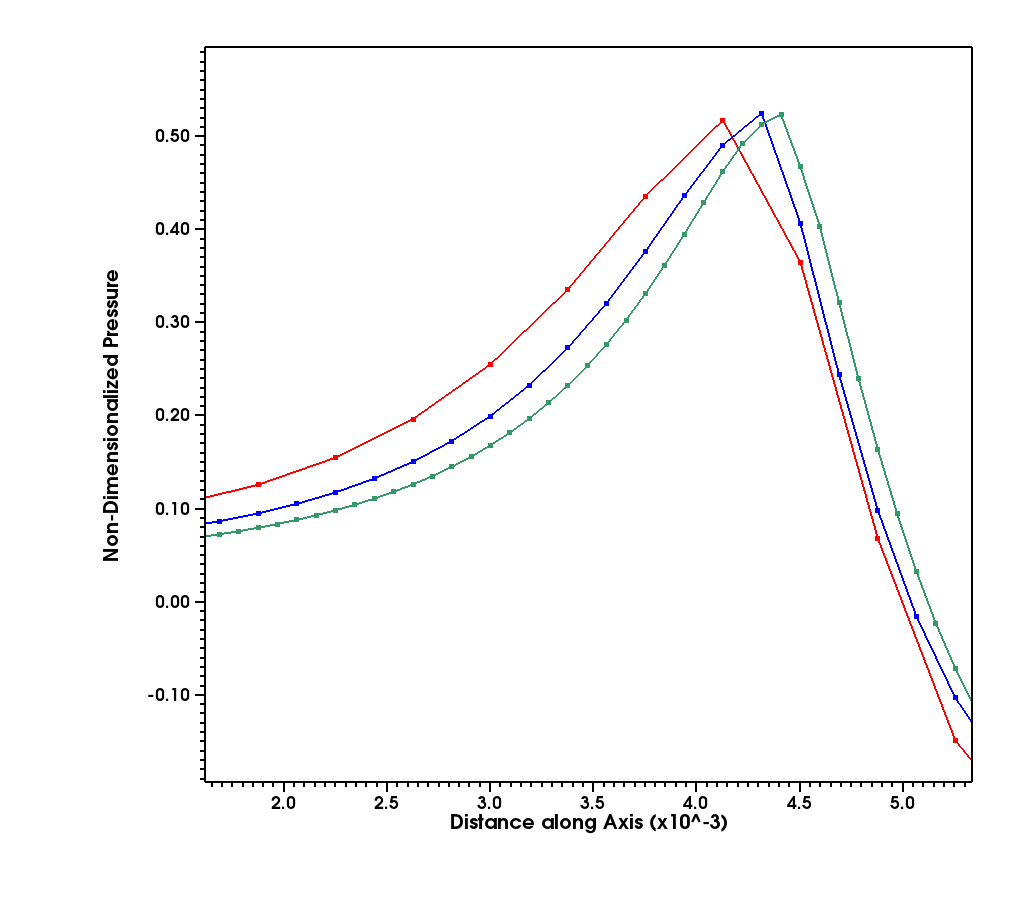
\includegraphics[width=0.45\textwidth]{Figures/Sagar/pressure_rd_MC.png} &
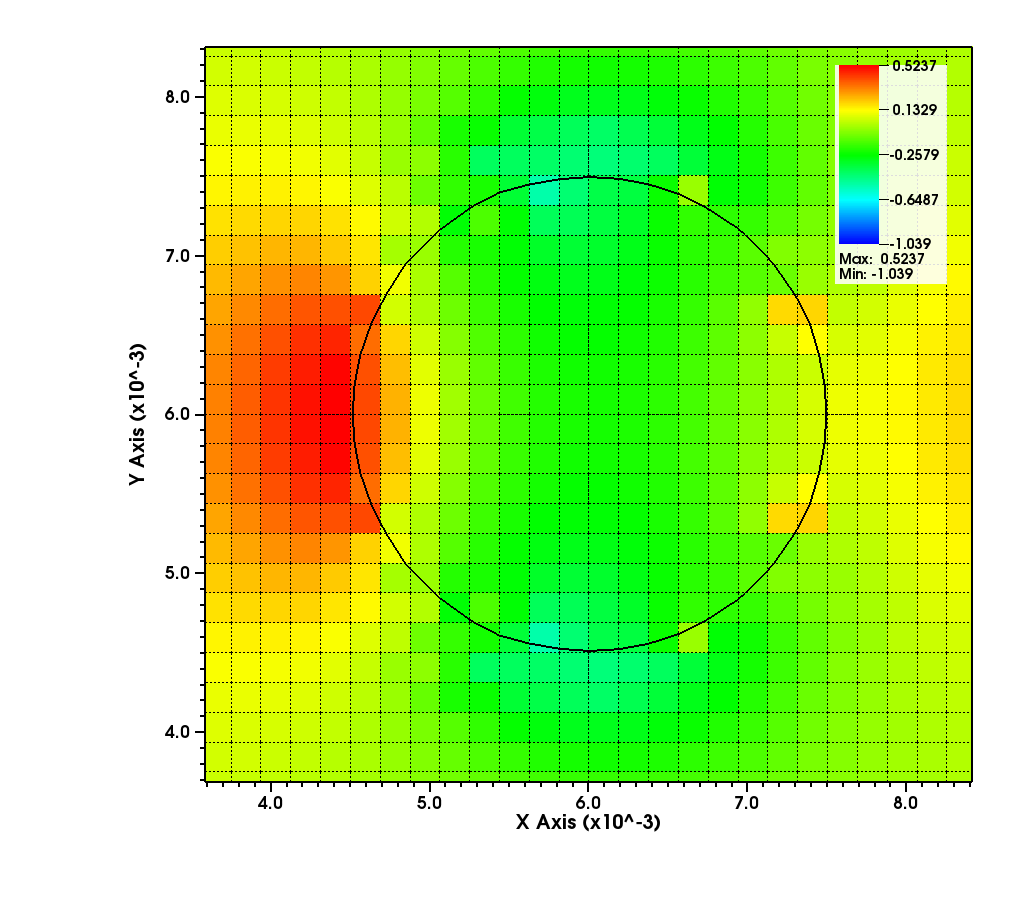
\includegraphics[width=0.45\textwidth]
{Figures/Sagar/16ppd_pressure_corrected.png}\\
(a) & (b)
\end{tabular}
\end{center}
\caption{ (a) The pressure profile on the axis a few timesteps after 
initialisation with the present 
method at various resolutions: $D/h = 8$ (red) , $16$ (blue) and $32$ (green). 
(b) The pressure distribution immediately after the start of the simulation 
using the present method and   $D/h = 16$.}
\label{FengXiao_corrected}
\end{figure}
% -----

\vspace*{0.2cm}

\begin{figure}[!h]
\begin{center}
\begin{tabular}{cc}
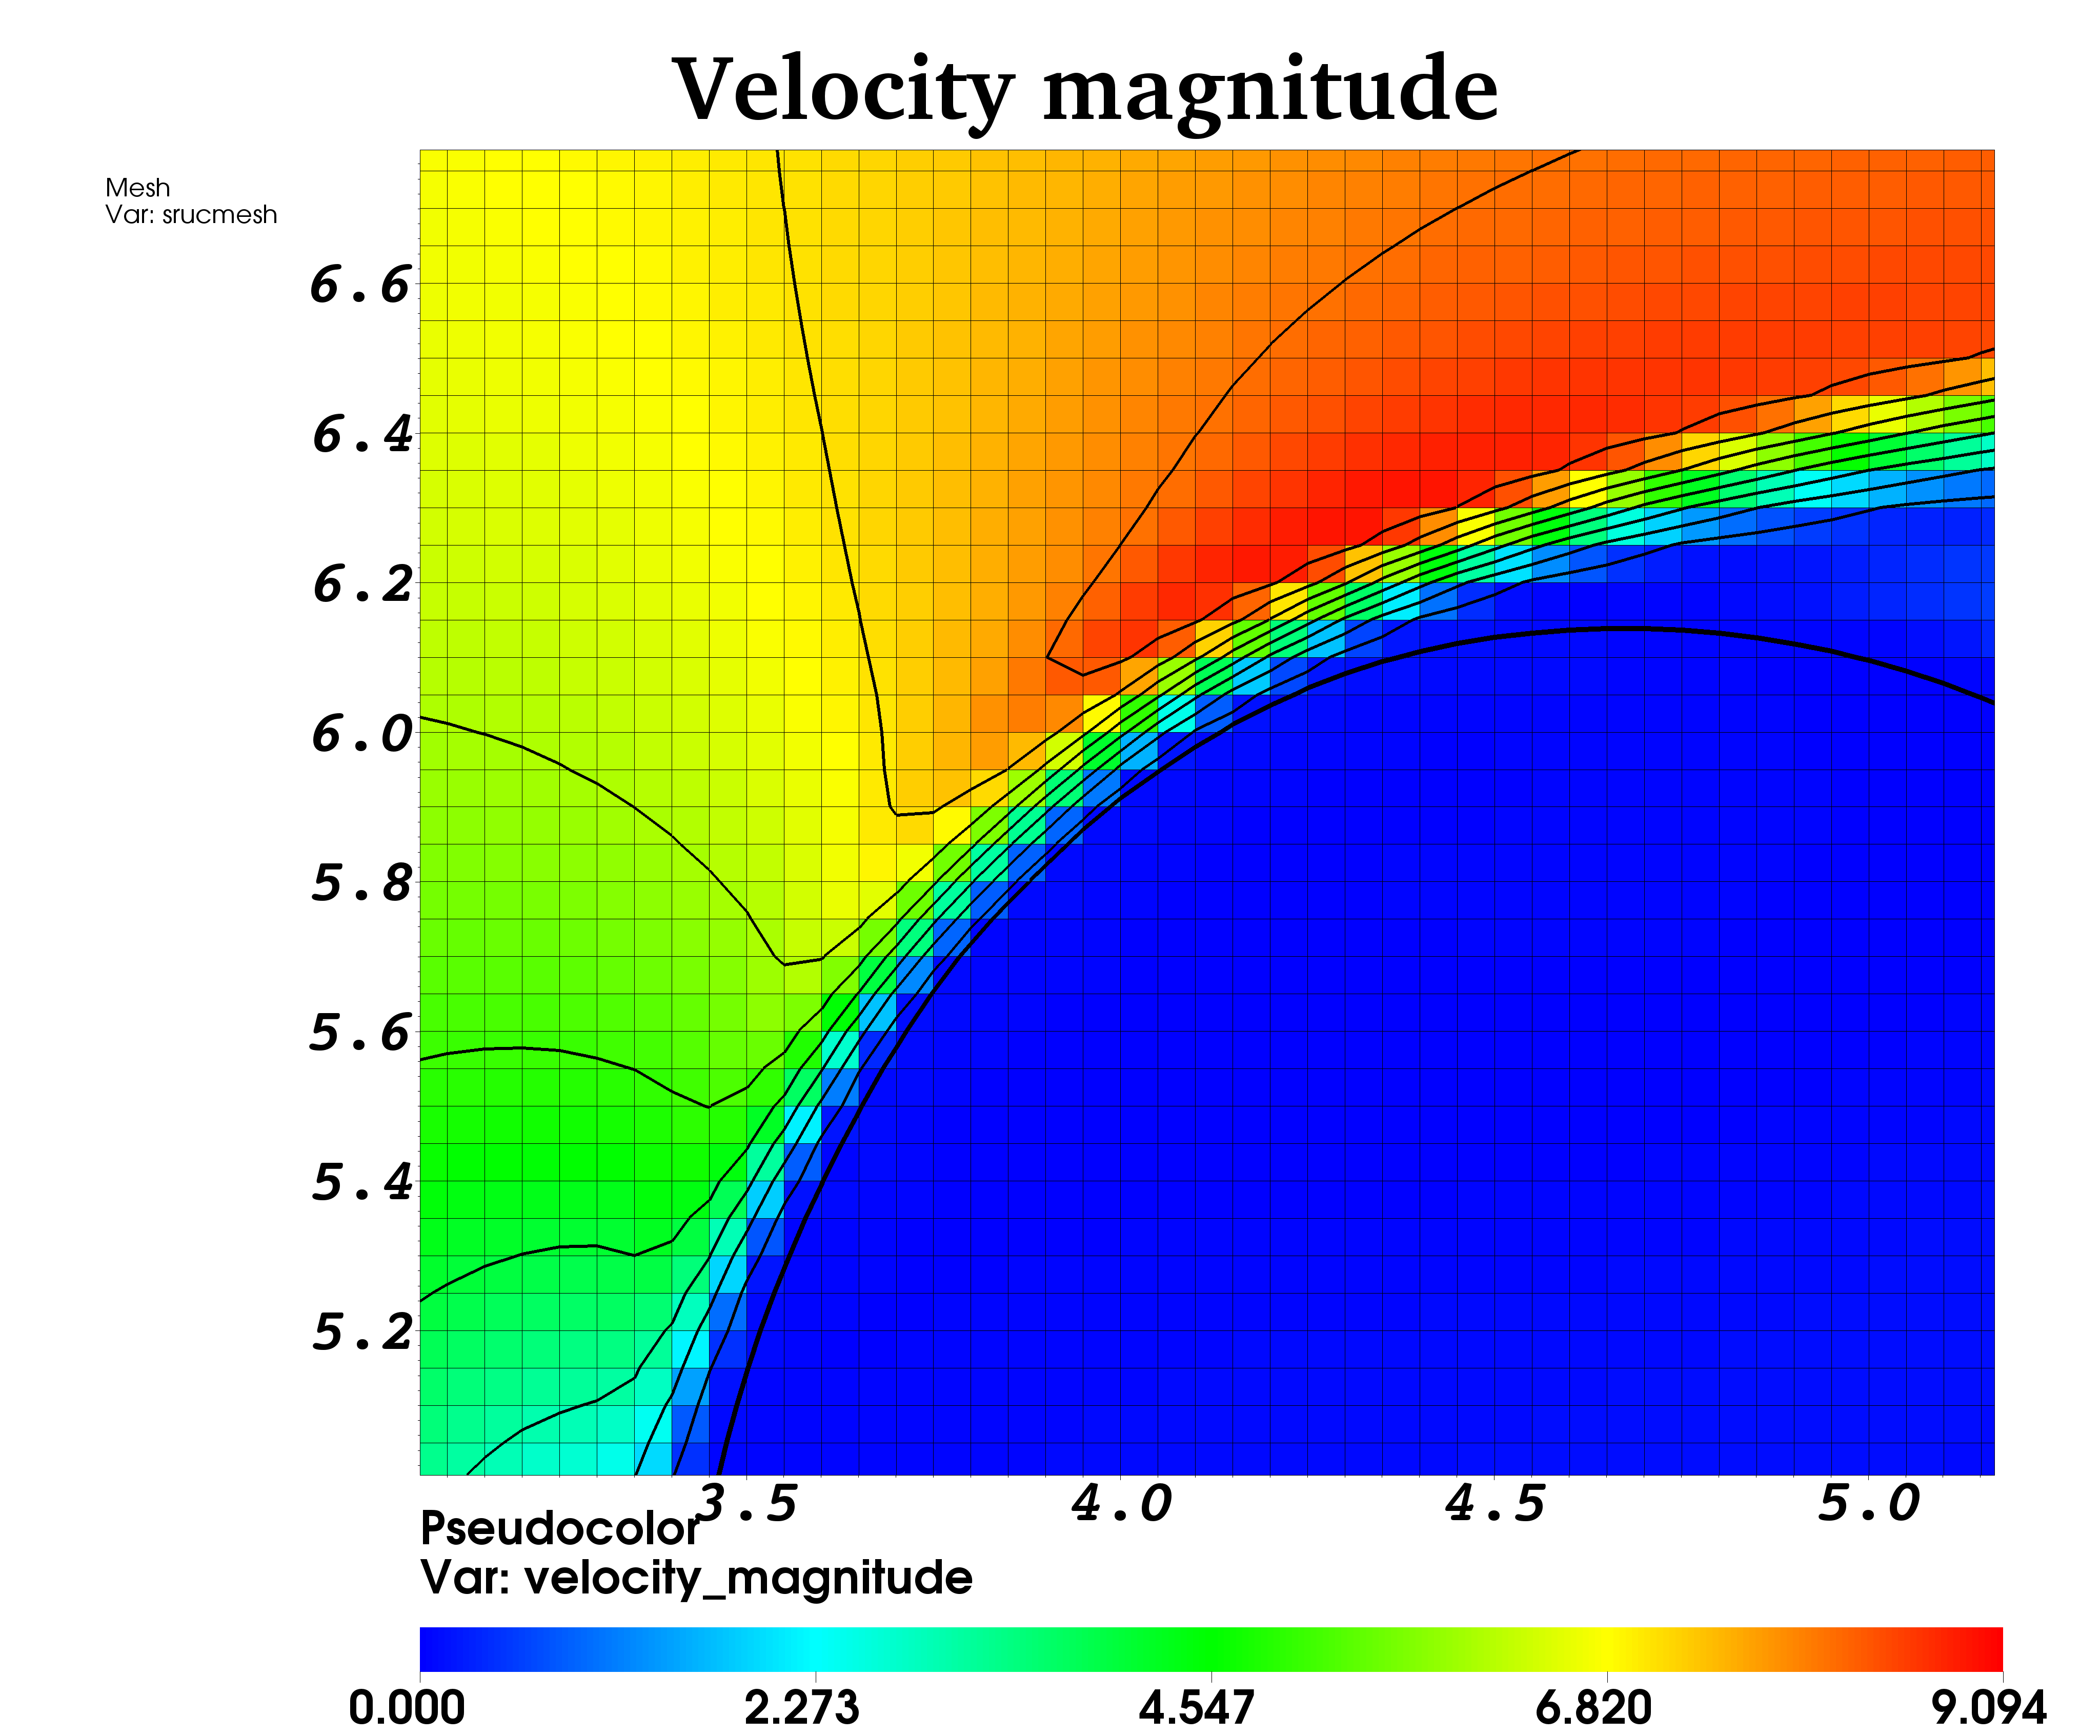
\includegraphics[width=0.42\textwidth]{Figures/vel.png}
& 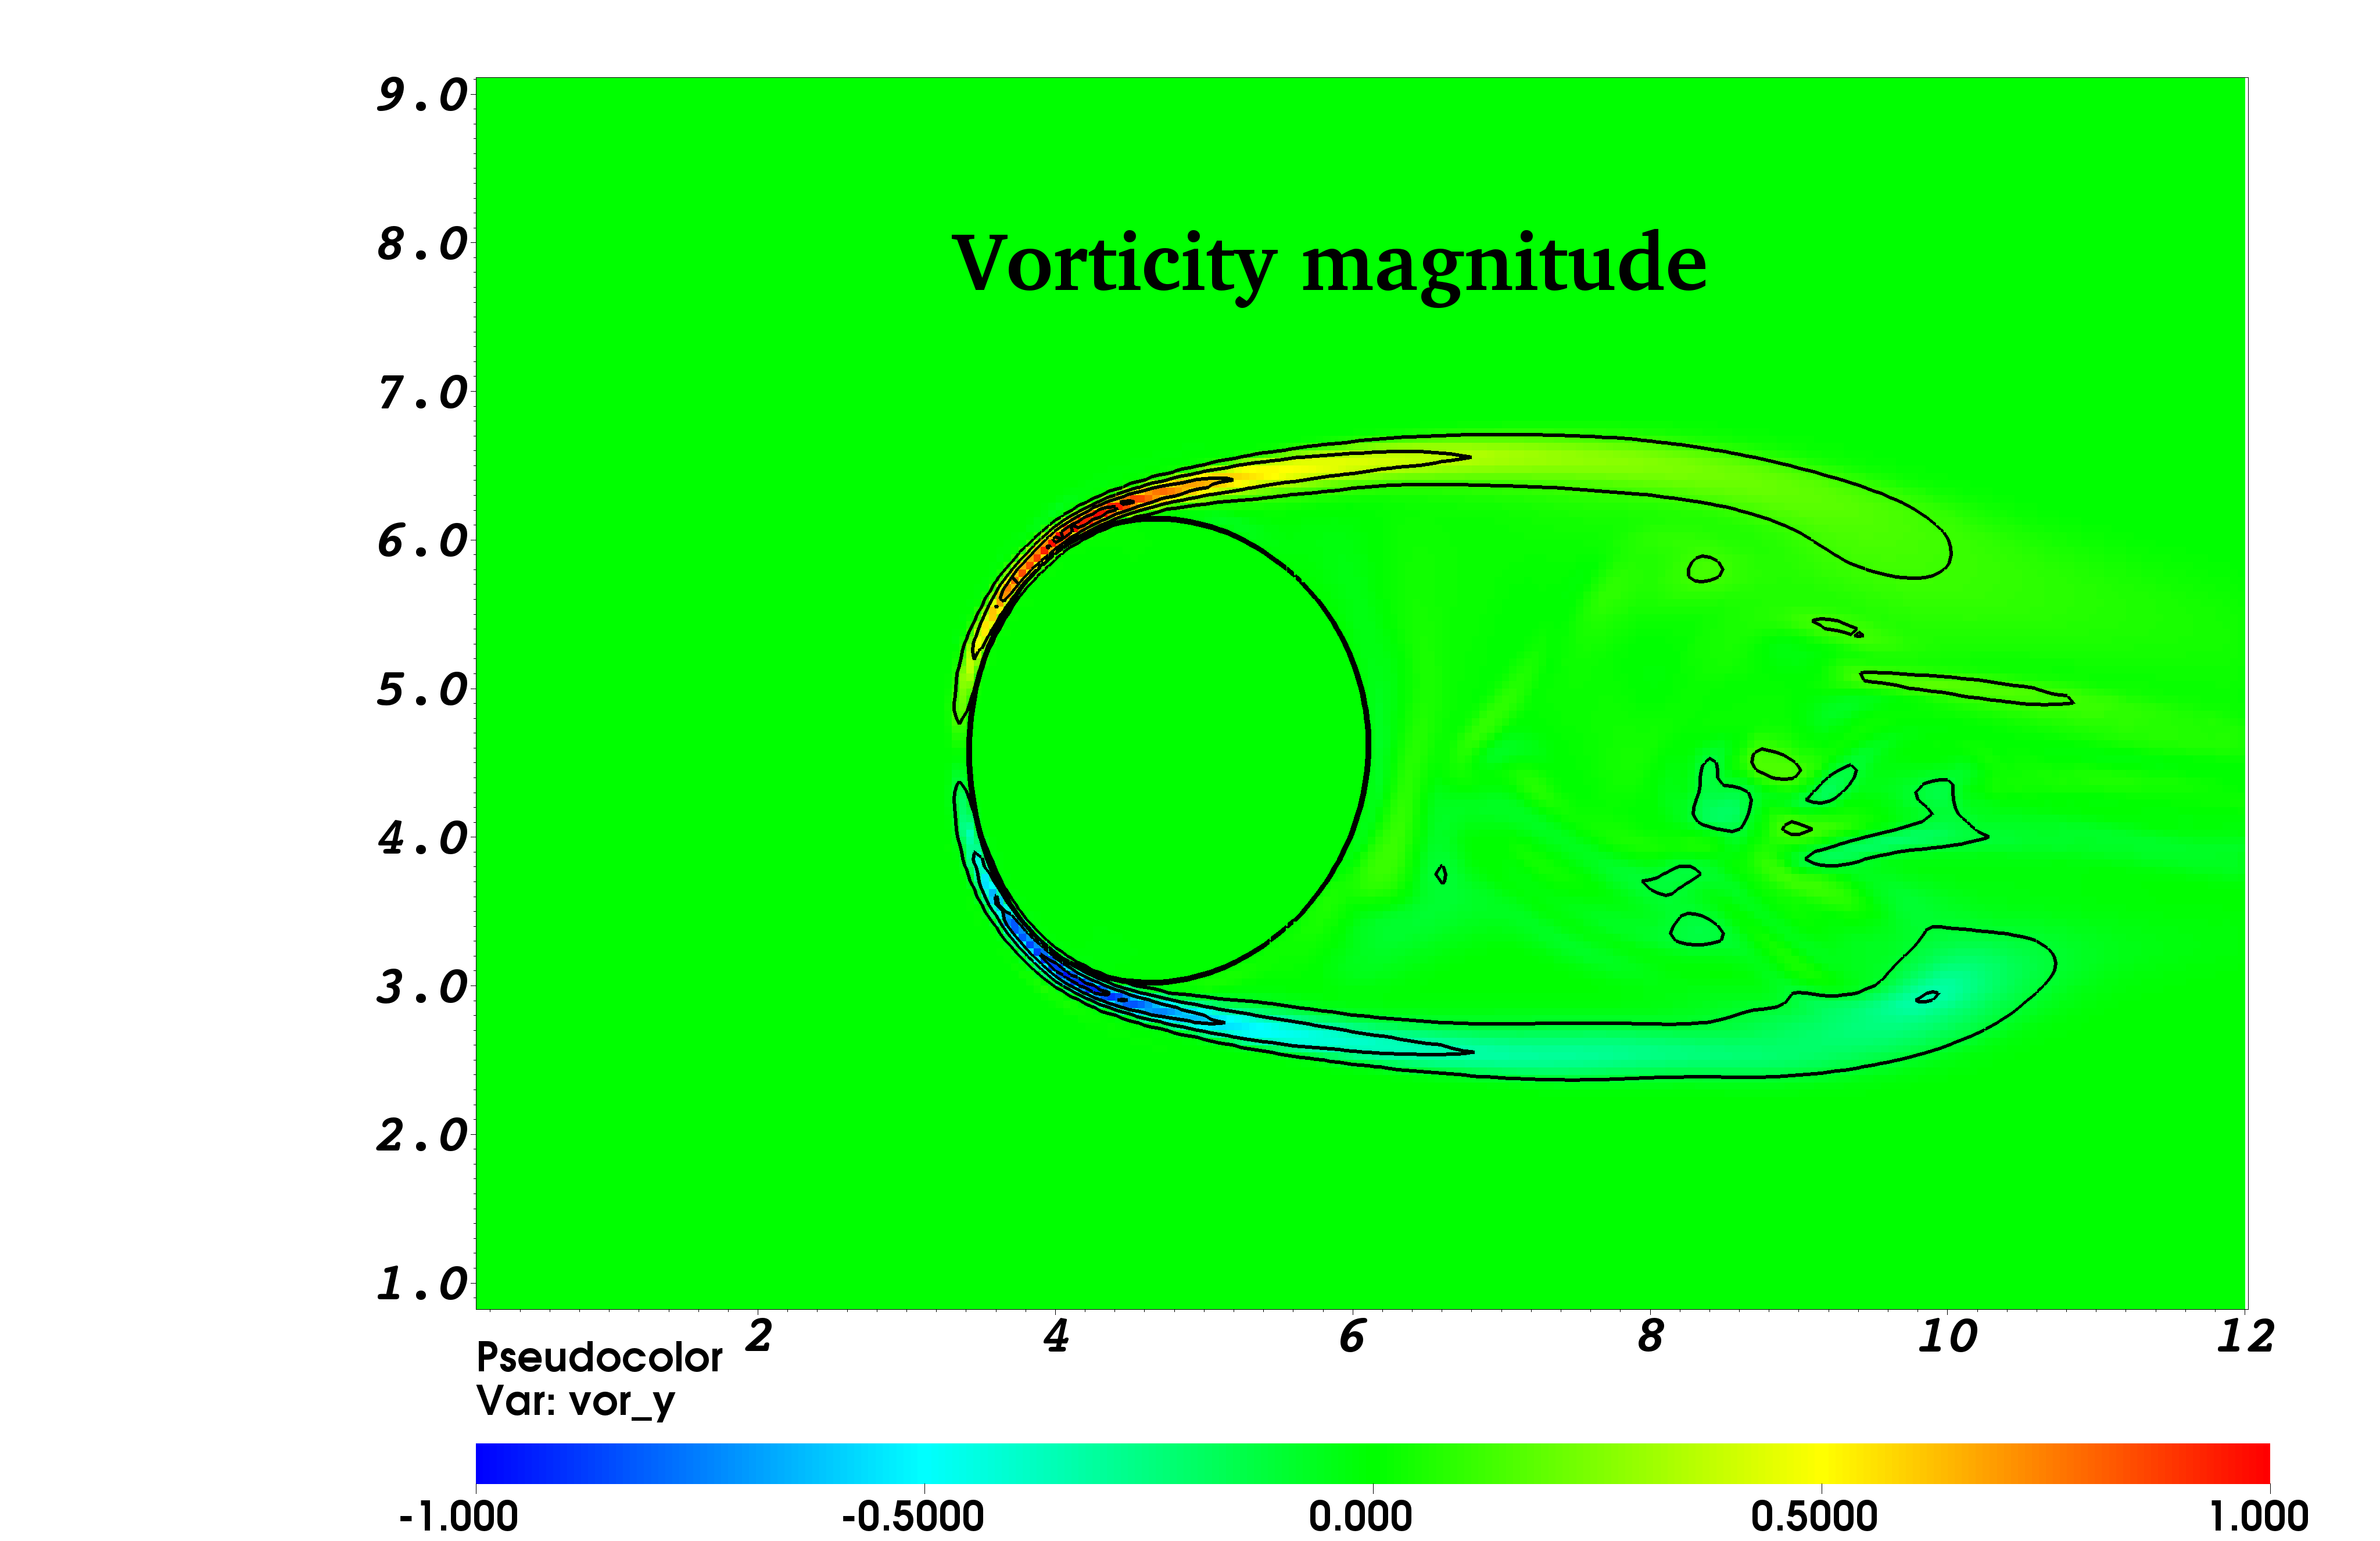
\includegraphics[width=0.48\textwidth]{Figures/vort.png} \\
(a) & (b)
\end{tabular}
\end{center}
\caption{Flow field around the 3 mm droplet with 60 grid points per diameter. 
(a) The velocity magnitude. It is seen that even at this highest resolution 
there are only three points in the boundary layer. (b) The vorticity magnitude. 
The marked separation of the boundary layers is observed with 
a more complex vortical region in the wake.}
\label{magn}
\end{figure}
% -----
\newcommand\DDD{{\cal D}}

Visualization of the flow around the droplets (Figure \ref{magn}) illustrates the challenging nature of the flow configuration, even for such a seemingly simple physical problem. As one can observe, the boundary layers are extremely thin, hence questioning our approximation that fluid velocity is continuous across the interface. We observe that applying the numerical method described in this paper brings a considerable and systematic improvement over a range of different flux limiters (WENO, ENO, Superbee, QUICK, Verstappen) and CFL numbers, as evidenced by comparing the figures \ref{FengXiao} and \ref{FengXiao_corrected}. To summarize, the simulations broadly fall in three categories: 

\begin{enumerate}
	\item They blow up anyway even while applying the present method
	\item They keep physical values of the kinetic energy and smooth interfacial shapes.
	\item They have a marked peak in kinetic energy as a function of time, associated with massively deformed interface shapes, 
\end{enumerate}

Regarding the first two points made above, we find that certain combinations of the advection scheme (CIAM/WY) and the flux limiter (ENO/WENO/Superbee/Verstappen/QUICK) display more numerical stability that the others, in particular, the most stable combinations of schemes are CIAM advection with Superbee limiter and the WY advection with QUICK limiter. As a minor remark, the CIAM advection with the Superbee limiter also appears to be quite diffusive. The third point highlights the systematic behavior of the simulations that are carried out without applying the present momentum-conserving method. 

\vspace*{0.2cm}

\begin{figure}[h!]
\begin{center}
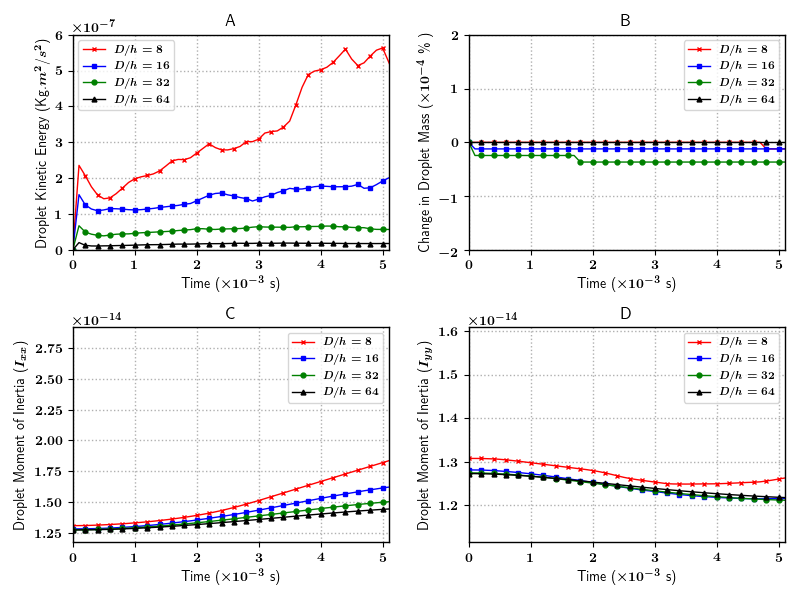
\includegraphics[scale = 0.6]{Figures/Sagar/multiplot_raindrop.png}
\end{center}
\vspace*{-0.5cm}
	\caption{Temporal evolution of quantities of interest to evaluate the performance of our present method for different spatial resolutions. (A) Kinetic energy of the droplet. (B) Percentage change in the droplet mass from initialized mass. (C) Moment of inertia of the droplet along flow (X) direction. (D) Moment of inertia of the droplet along direction perpendicular to flow (Y,Z), evolution of $I_{yy}$ is identical to $I_{zz}$, thus the latter is not shown.}
\label{multi}
\end{figure}

We illustrate the performance of the present method through the results of our simulations in Figure \ref{multi}. We have carried out simulations corresponding to $D/h = 8, 16, 32 $ and $64$, while keeping the same value for the inflow velocity boundary condition. The quantities of interest while examining the robustness of the method are the temporal evolution of the droplet kinetic energy (Fig. \ref{multi}. A) and droplet mass (Fig. \ref{multi}. B), as well as moment of inertia of the droplet along directions aligned to the inflow velocity (Fig. \ref{multi}. C) and orthogonal (Fig. \ref{multi}. D) to it. The moment of inertia is used as a descriptor of the 'average' droplet shape, with the three moments of inertia along the different axes $I_m$ defined as - 

\be
I_m = \int_\DDD H x_m^2 {\rm d}\X \;, \quad  1 \le m \le 3,
\nd

where $\DDD$ is the computational domain and $x_m$ is the distance of the interface relative to the center of mass of the droplet.   

\begin{figure}[h!]
\begin{center}
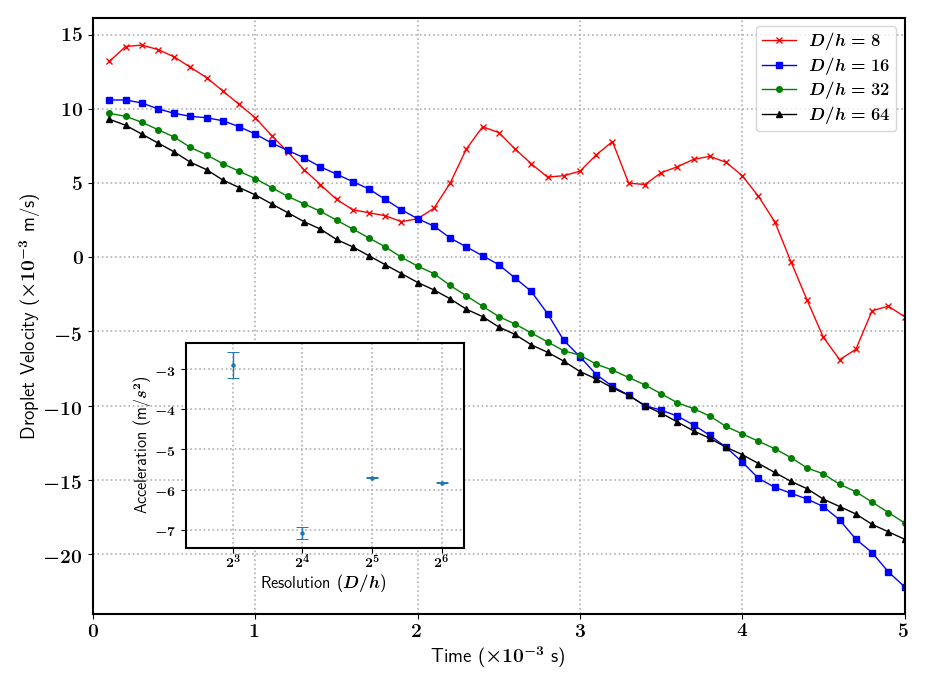
\includegraphics[scale = 0.5]{Figures/Sagar/dropl_velocity_accel_ppd.png}
\end{center}
\vspace*{-0.5cm}
\caption{Comparison of droplet velocity as a function of time, for different droplet resolutions, The droplet velocities correspond to that of their respective center of masses. Inset : Convergence of the droplet acceleration as a function of resolution, computed using the best linear fit over the temporal variation of their respective velocities. The error bars signify the asymptotic standard error (least-squares) corresponding to the obtained linear fits.} 
\label{drop_vel}
\end{figure}

The kinetic energy of the droplet evolves in a relatively smooth manner, without the presence of sudden spikes and falls which are emblematic of the non-conservative version of our method. Such abrupt changes in kinetic energy of the droplet have been found to be associated with instants when the droplet undergoes 'artificial' atomization or breakup, henceforth resulting in the catastrophic loss of stability for the numerical method. We observe a systematic drop in the amount of the droplet kinetic energy as we increase resolution, with the most probable explanation being that of the suppression of spurious interfacial oscillations which are rampant at low resolutions. There is also a component of the kinetic energy of the droplet associated with the internal coherent vortical structures generated due to the interaction of aerodynamic shear at the interface, evidenced by the non-zero value of the kinetic energy even for the most highly resolved droplets. In terms of mass conservation, our method performs exceedingly well, with the fractional loss of mass bounded within $0.0001 \%$ for all droplet resolutions tested. Finally, the moment of inertia of the droplet appears to evolve in a smooth manner for all droplet resolutions, with higher resolutions exhibiting lower amounts of inertia as a result of the more compact shapes obtained once the spurious interfacial deformation modes are subdued.          

\begin{figure}[h!]
\begin{center}
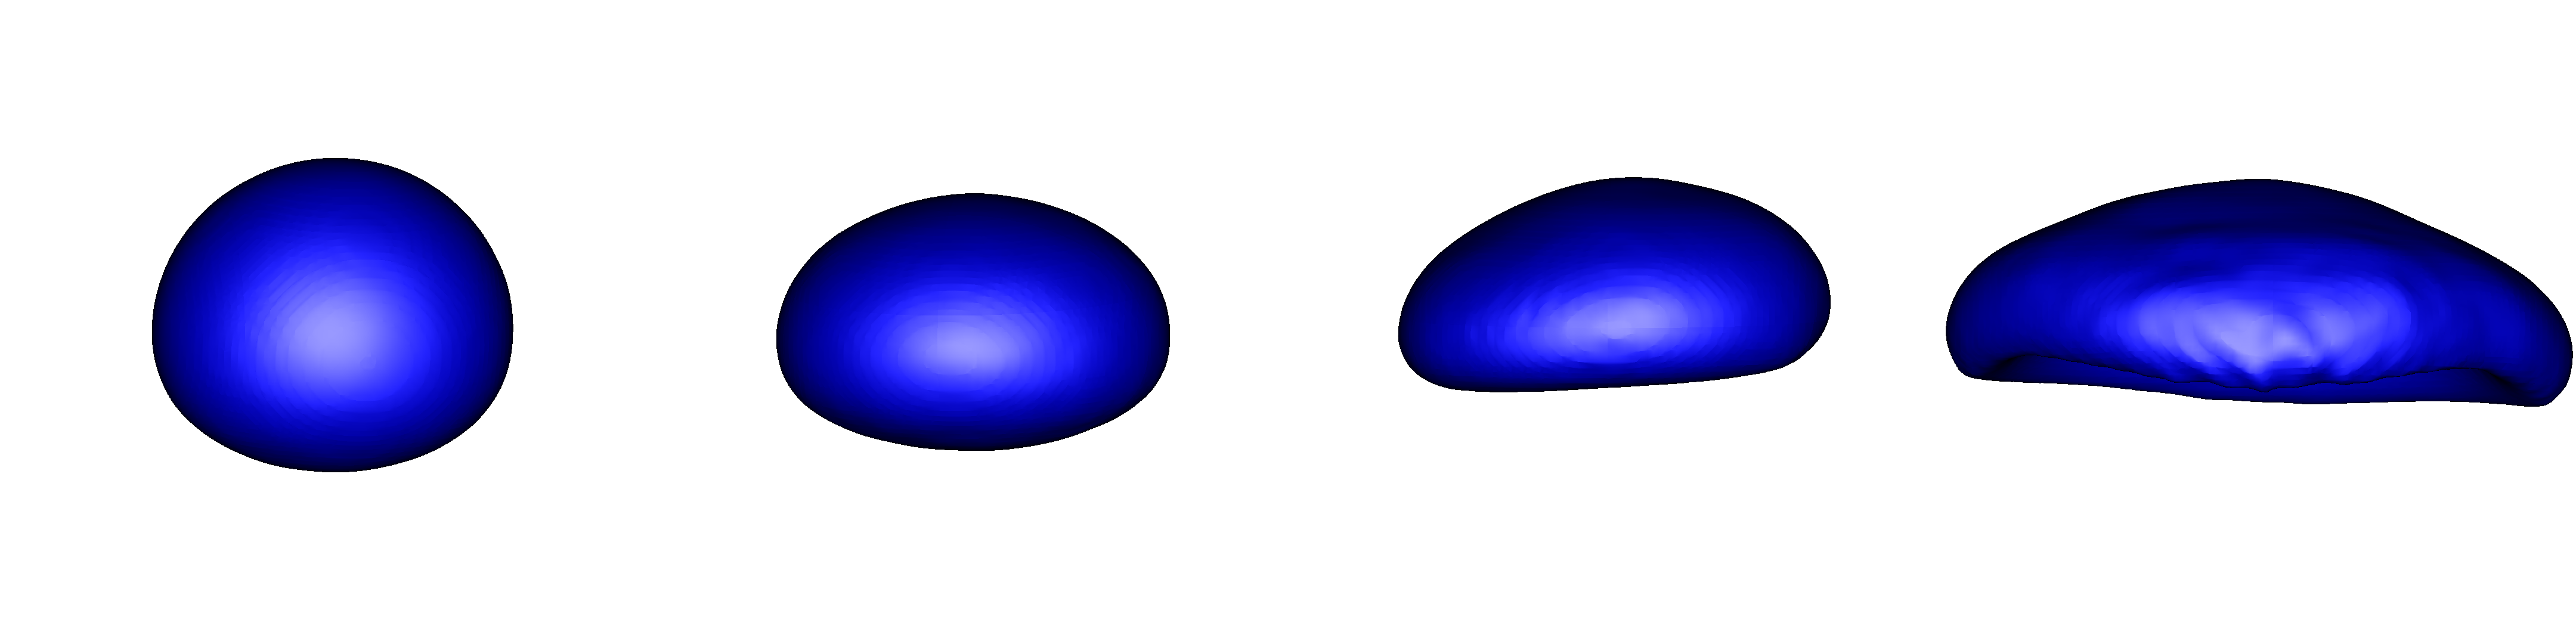
\includegraphics[width=0.99\textwidth]{Figures/flatten.png}
%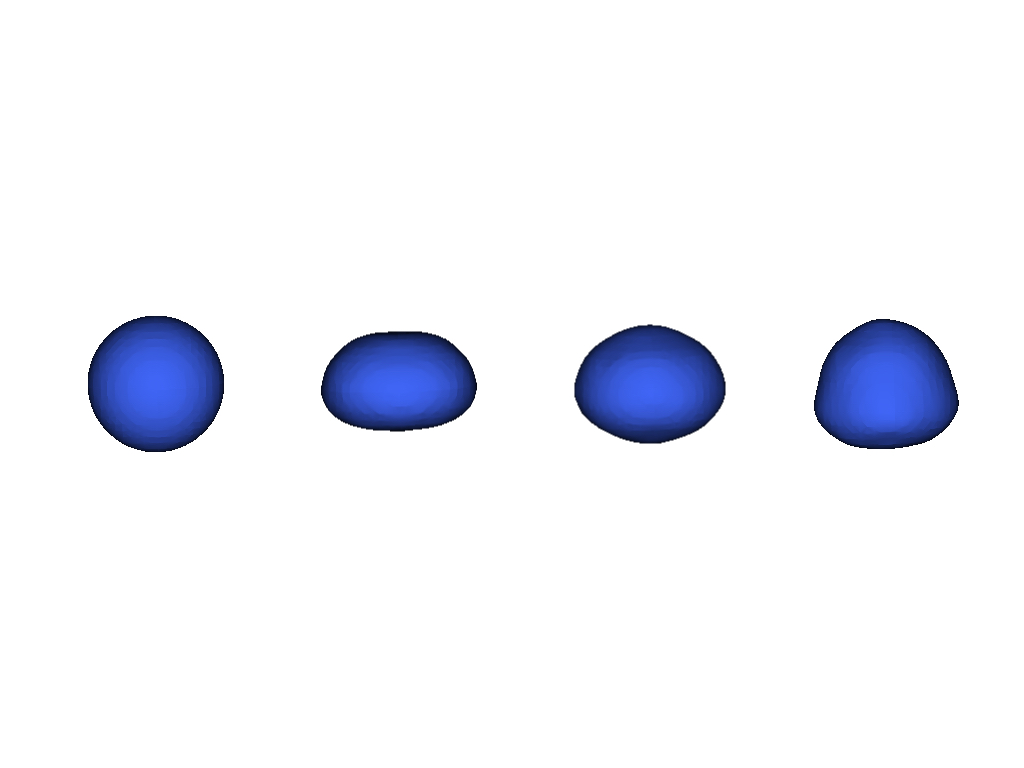
\includegraphics[width=0.99\textwidth]{Figures/Sagar/fig14-001.jpeg}
\end{center}
\caption{Flattening of the droplet with increasing equivalent diameter 
(see text). From left to right $D_e=3, \,4.6,\, 6.4$ and $8\, mm$.}
\label{flatten}
\end{figure}
% -----

From the values of the moments of inertia, the horizontal and vertical 
extents of the droplet (respectively $D_r$ and $D_x$) can be found 
and compared to the values found by the authors of \cite{Reyssat:2007ko}. 
We find $D_r=3.1 \,mm$ and $D_x=2.6 \,mm$, while ref. \cite{Reyssat:2007ko} 
concludes that drops are quasi-spherical for an equivalent diameter 
$D_e \le l_c$ and deformed for $D_e > l_c$, where $l_c =(\sigma/\rho g)^{1/2}$ 
is the capillary length, $l_c = 2.7 \,mm$ for water. 
Indeed repeating the simulations for larger drops we find increased 
flattening as shown on Figure \ref{flatten}. 

We have to keep in mind that the velocity inflow condition does not correspond to the 'exact' teminal velocity field an actual falling raindrop might experience, hence the droplet in our numerical setup does have some finite acceleration due to the imbalance between the aerodynamic forces and gravity. In Figure \ref{drop_vel}, we demonstrate the velocity of the center of mass of the droplet as a function of time, and its behavior as we increase the droplet resolution. As one can observe, due to the imbalance of forces acting on the droplet, it undergoes a net acceleration as evidenced by the approximately linear increase (absolute value) in the velocity as a function of time. The temporal variation in the droplet velocity is fitted to a linear polynomial in order to evaluate the droplet acceleration by means of a standard least-squares approach, for each droplet resolution. We illustrate (inset Figure \ref{drop_vel}) that we achieve more accurate fits as a consequence of higher droplet resolutions, as evidenced by decrease in the standard error on the fits ranging from $\pm 11.1 \%$ for $D/h = 8$ to a value of $\pm 0.12 \%$ for the highest resolution of $D/h = 64$. This provides us with an indirect indication that our numerical method can be used to generate high fidelity models of the underlying dynamics, provided sufficient resolution.           


%
%\clearpage

% Slightly less stable methods result when one takes $\hat x = x_i$. 
% In that case we observe at low resolution ($D/h=15$) the energy spike shown 
% in Figure \ref{lowres}. The energy spike is 
% associated with a moving bump on the droplet. Using a higher resolution 
% of $D/h=30$ makes the energy spike disappear. 
% Switching to the shifting of the interpolation point $\hat x$ described in 
% Section \ref{tunedinter}, even more stable behavior is observed, down 
% to resolutions of $D/h=8$. 
% -----
% \begin{figure}
% \begin{center}
% \begin{tabular}{cc}
% 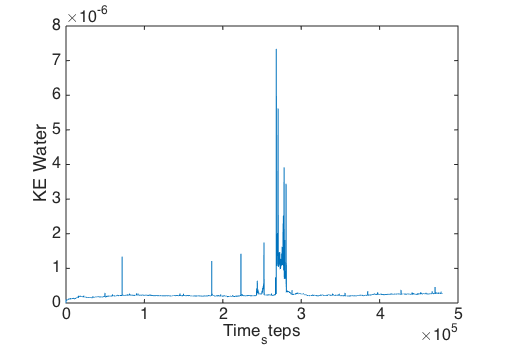
\includegraphics[width=0.5\textwidth]{Figures/KE.png}
% & 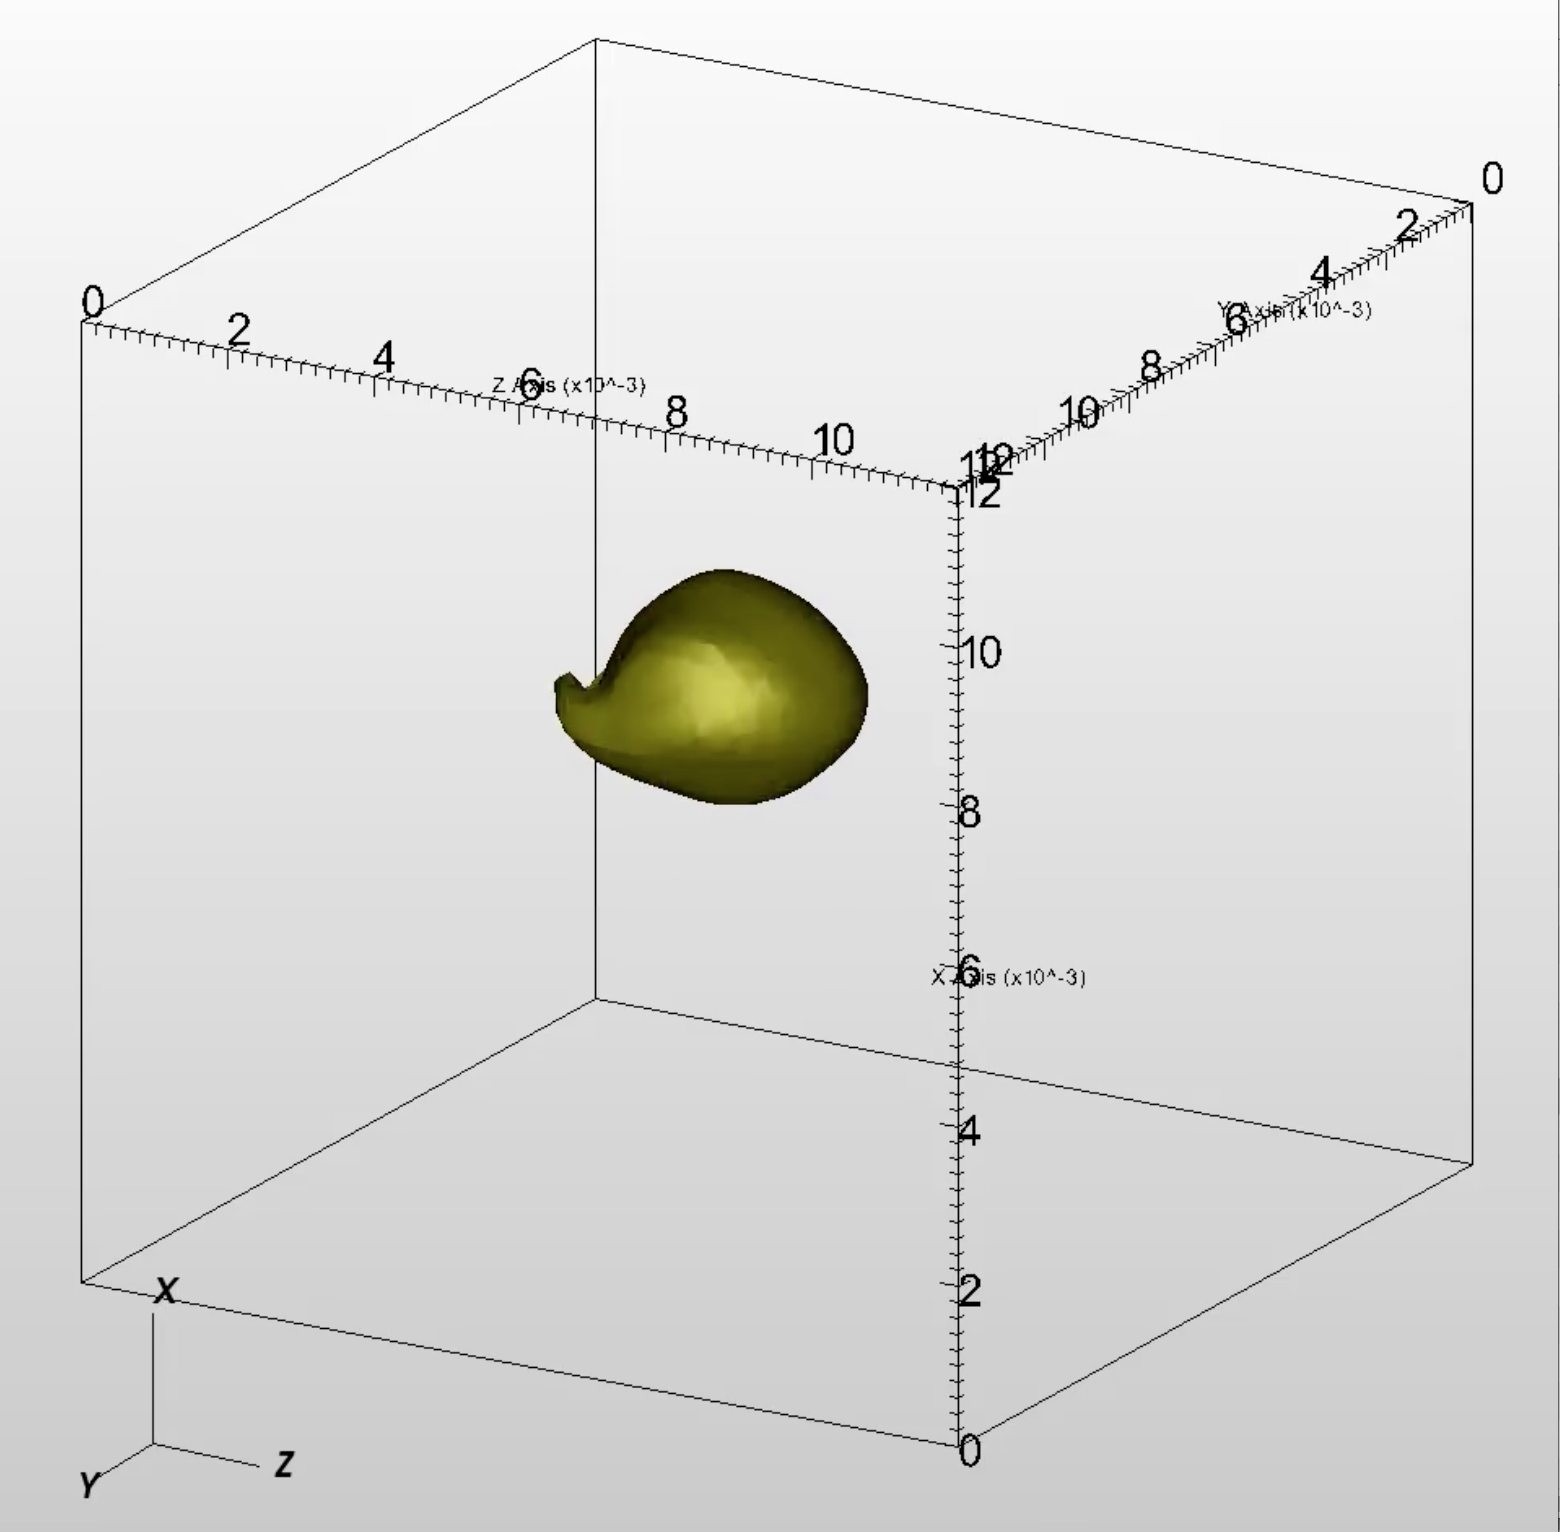
\includegraphics[width=0.4\textwidth]{Figures/bump.png} \\
% (a) & (b)
% \end{tabular}
% \end{center}
% \caption{Effect of a slightly unstable setup. (a) The kinetic energy 
% as a function of time exhibits several
% spikes (b) A snapshot of the simulation at the instant of the formation 
% of the first spike. A pointed
% bump forms on the droplet and starts rotating rapidly.}
% \label{lowres}
% \end{figure}
% -----
%% -----
%\begin{figure}
%\begin{center}
%\begin{tabular}{cc}
%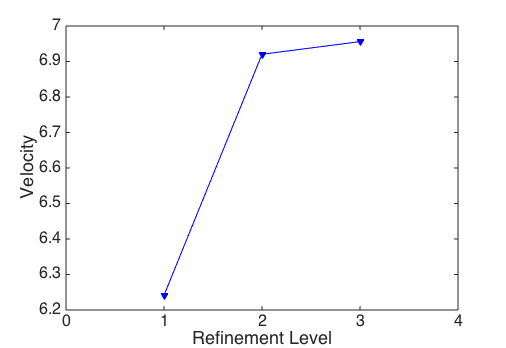
\includegraphics[width=0.45\textwidth]{Figures/veloconv.png}
%& 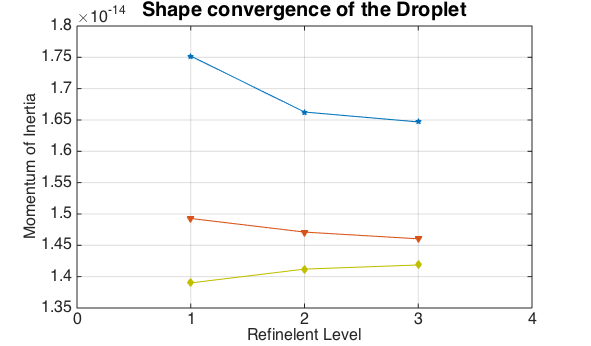
\includegraphics[width=0.45\textwidth]{Figures/shapeconv.png} \\
%(a) & (b)
%\end{tabular}
%\end{center}
%\caption{Convergence of simulations. (a) Evolution of the terminal velocity 
%with grid refinement. (b) Evolution of the three moments of inertia with 
%grid refinement.}
%\label{converge}
%\end{figure}
%% -----
% -----



\subsection{Atomizing air and water planar jets}

We also test the capability of the VOF-consistent momentum-conserving scheme 
to simulate complex air-water flows with an unstable shear flow. For that 
purpose we repeat the setup of reference \cite{Ling16}. Two jets of air and water 
are entering the computational domain from the left of Figure \ref{atom}
at velocities comparable to those of experiments. However in order to 
save computational time the domain is smaller than in experiments. Physical 
properties of air and water are identical to those of the falling raindrop case 
given in Table \ref{raindropprop}. The flow and domain characteristics are 
given in Table \ref{PhysicalParam} including a gas boundary layer 
and separator-plate size identical to those of reference \cite{Ling16}. 
The notations are as in reference \cite{Ling16}: $H_p$ is the thickness of the
jet of phase $p$, there is a separator plate of thickness $l_y$ and a 
gas boundary layer of thickness $\delta_g$.  The two streams have 
equal thickness $H_l=H_g$. The dimensionless parameters are given in 
Table \ref{dimensionlessParam}. The CIAM advection method has been used. 
The number of grid points in the layer $H_l/h = 16$ is relatively small
(compared to the  $H_l/h = 32$ in the smallest (coarsest) simulation
of reference \cite{Ling16}). It is thus all the more remarkable that the 
simulation is stable since using a smaller number of grid points usually 
increases the trend towards instability. It is interesting to note 
that the VOF calculations accounts for 31.5\% of the total time, while the 
inversion of the Poisson operator for the pressure accounted for 51.5\%. 
The whole simulations runs overnight on a present-day workstation. 

% -----
\begin{figure}
\begin{center}
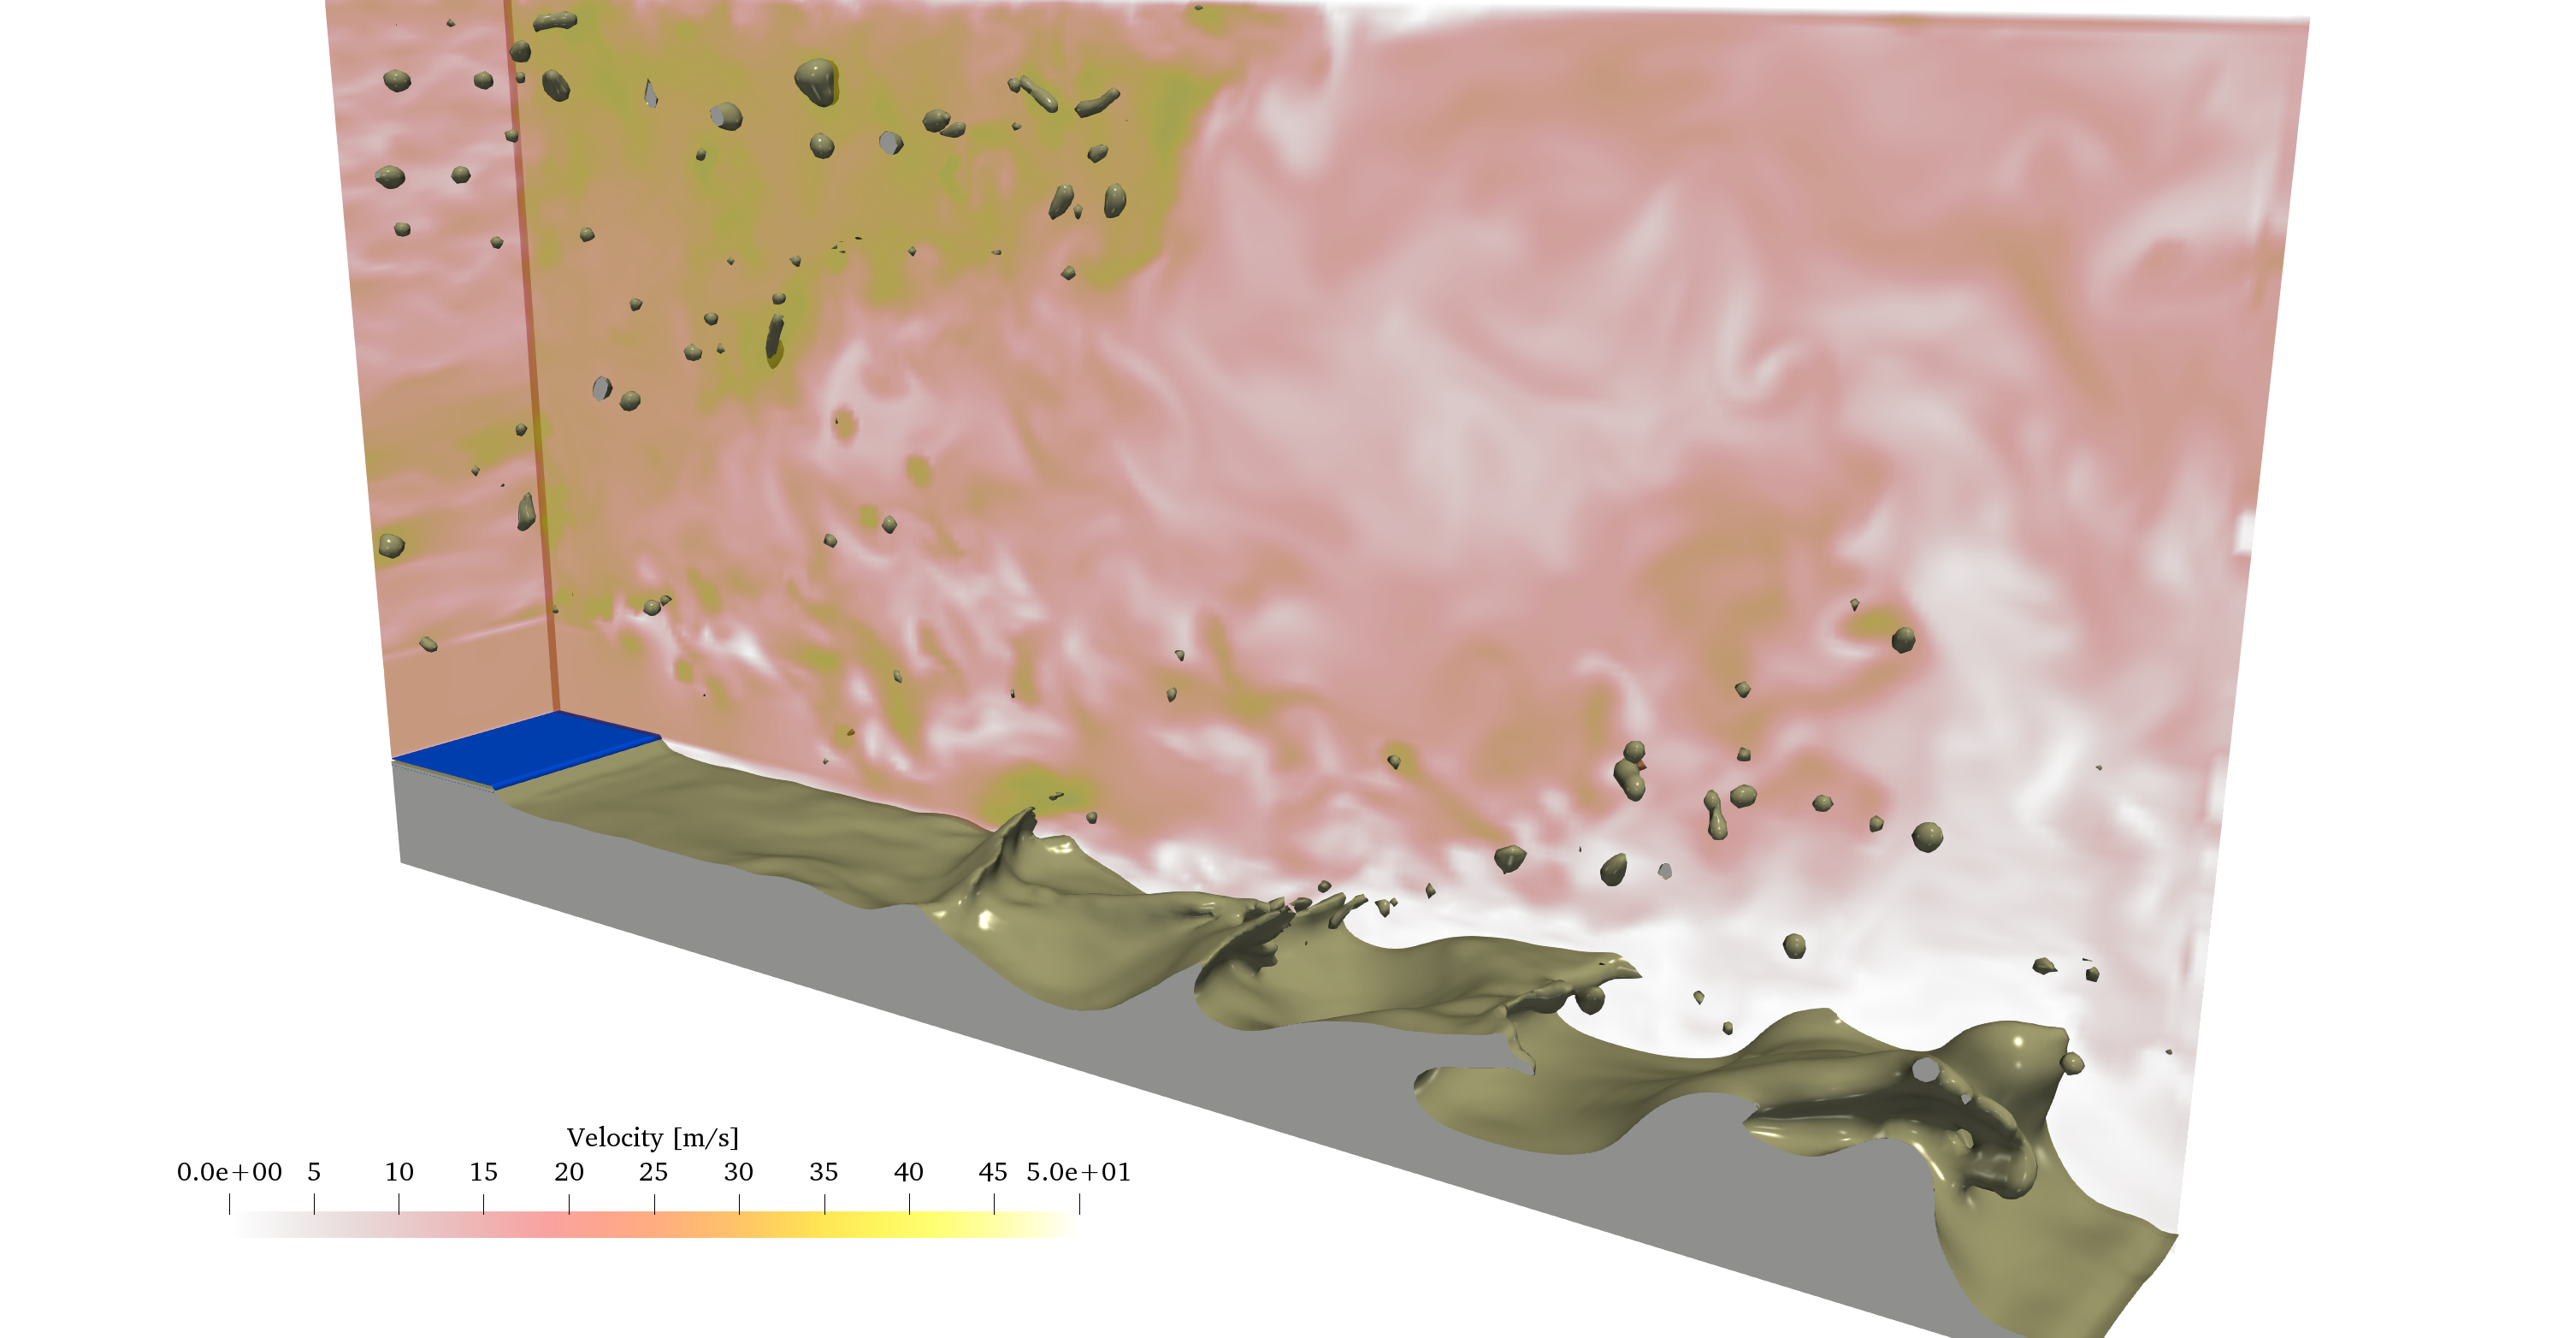
\includegraphics[width=0.99\textwidth]{Figures/Marco/vof-vel-atom.png}
\end{center}
\caption{Atomizing layer with air/water properties.}
\label{atom}
\end{figure}
% -----

% -----
\begin{table}
\begin{center}
\begin{tabular}{cccccc}
\hline
\hline
 $U_l$ & $U_g$ & $H_l$ & $h$ & $l_y$ & ${\delta_g}/{l_y}$ \\

 $(m/s)$ & $(m/s)$ & $(m)$ & $(m)$ & $(m)$ & $(-)$ \\
\hline
 $1$ & $25$ & $4\, 10^{-3}$ & $2.5\, 10^{-4}$ & $2.5\, 10^{-4}$ & $2$\\
\hline
\hline
\end{tabular}
\end{center}
\caption{Physical parameters (defined in the text) for the atomizing layer setup. The fluid 
properties are the same as in Table~\ref{raindropprop}.
}
\label{PhysicalParam}
\end{table}
% -----

% -----
\begin{table}
\begin{center}
\begin{tabular}{cccccc}
\hline
\hline
 $M$ & $r$ & $m$ & $\Re_{g,\delta}$ & $\We_{g,\delta}$  & $\Re_{g}$ \\
 $\rho_g U_g^2/\left(\rho_l U_l^2\right)$ & $\rho_l/\rho_g$ 
 & $\mu_l/\mu_g$ & $\rho_g U_g H_g/\mu_g$ & $\rho_l U_l H_l/\mu_l$ 
 & $\rho_g U_g^2 H_g/\sigma$ \\
\hline
 $0.75$ & $831.8$ & $45$ & $757.6$ & $5.151$ & $6061$  \\
\hline
\hline
\end{tabular}
\end{center}
\caption{Dimensionless parameters for the atomizing layer setup.}
\label{dimensionlessParam}
\end{table}
% -----


\section{Conclusion}

We have presented and tested a simulation method for multiphase flow
that shows increased stability at large density contrasts and large
Reynolds numbers. The method is closely related to some variants of
the VOF method including an implementation of the WY advection method. 
The increased stability is evidenced in the test case
of a single $3$-mm droplet of water falling in air, a typical
raindrop. It is a reflection on the challenging nature of multiphase
flow that such complex methods apparently need to be implemented to
resolve such an everyday and simple phenomenon.

The method comes with a significant saving of computer time, since for 
similar problems with raindrops, our attempts with a non-momentum-conserving
VOF approach led to catastrophic deformation of the drop or strong dimple 
formation. These problems have also been observed by us using other 
non-VOF-consistent and non-momentum-conserving methods such as the one of 
\cite{popinet09}. In that case whenever less than 200 grid points per 
diameter are used numerically stable air-water 
drops accelerated at moderate Weber number cannot be found. However for
higher resolutions they can be computed without difficulty as also found 
by the authors of ref. \cite{Jain15}.
Here, approximate solutions accurate within 15\% are found with only 15 
points per diameter, and non-divergent computations are found with as little 
as 2 points per diameter. 

A particular advantage of the method is that it is conserving mass at the 
accuracy at which discrete incompressibility is enforced and opens a
perspective for similar momentum conservation using WY advection.
The method nevertheless is more complex and costly than a colocated method. 
This opens the perspective for systematic development of other methods with 
different grid arrangements. Another perspective is the potential
of stable methods with large density contrasts, exact mass and momentum conservation 
and small droplets, that could be smoothly merged into models that represent 
the small droplets as Lagrangian Point Particles \cite{Ling15}.

\section{Acknowledgements} % All authors

This work has been supported by the ANR MODEMI project (ANR-11-MONU-0011) program and grant 
SU-17-R-PER-26-MULTIBRANCH from Sorbonne Universit\'e.
%
Philipp Yecko acknowledges support from grants NSF-1362823 and NSF-1620158.
%

This work was granted access to the HPC resources of TGCC-CURIE, TGCC-IRENE and CINES-Occigen under the allocations 
t20152b7325,  t20162b7760, 2017tgcc0080 and A0032B07760, made by GENCI and TGCC. 
The authors would also acknowledge the MESU 
computing facilities of Sorbonne Universit\'e. 

We would thank Dr.\ W.\ Aniszewski, Dr S. Dabiri, Dr Jiacai Lu and Dr. P. Yecko for their contribution to the development of the code \emph{PARIS-Simulator}, and we thank   Dr.\ W.\ Aniszewski, Dr. V. Le Chenadec, Mr. C. Pairetti, Dr. S. Popinet and Dr. S. Vincent for useful conversations on the topics of this paper.  

Finally, the simulation data are visualized by the software VisIt developed by the Lawrence Livermore National Laboratory. 
%% The Appendices part is started with the command \appendix;
%% appendix sections are then done as normal sections
%% \appendix

%% \section{}
%% \label{}

%% If you have bibdatabase file and want bibtex to generate the
%% bibitems, please use
%%
%%  \bibliographystyle
%%  \bibliography{<your bibdatabase>}

%% else use the following coding to input the bibitems directly in the
%% TeX file.
\section*{References}
\bibliographystyle{elsarticle-num} 
\bibliography{multiphase,gretar}
\appendix
\section{Kelvin Helmholtz instability: numerical setup}
We consider the 2D base flow shown on Figure \ref{khappfig}. Coordinates are noted $(x,z)$ and vectors
$(u,w)$. The height of the interface is $h(x,t)$. The flow has density $\rho_1$ for $z<h(x,t)$ and 
$\rho_2$ for $z>h(x,t)$ and is incompressible. The base flow is a parallel shear flow.
The base flow is uniform with $u=-U$ for $z<0$
and $u=U$ for $z>2a$, with a linear (Couette flow) boundary layer in between.  When $\rho_1 \neq \rho_2$ the heavier fluid is the ``liquid'' and the lighter the ``gas''. For $\rho_1 > \rho_2$ the boundary layer is in the gas while otherwise the bounary layer is in the liquid. 
Similar flows have been studied
in \cite{Matas_2011a,Eggers08}.

\begin{figure}
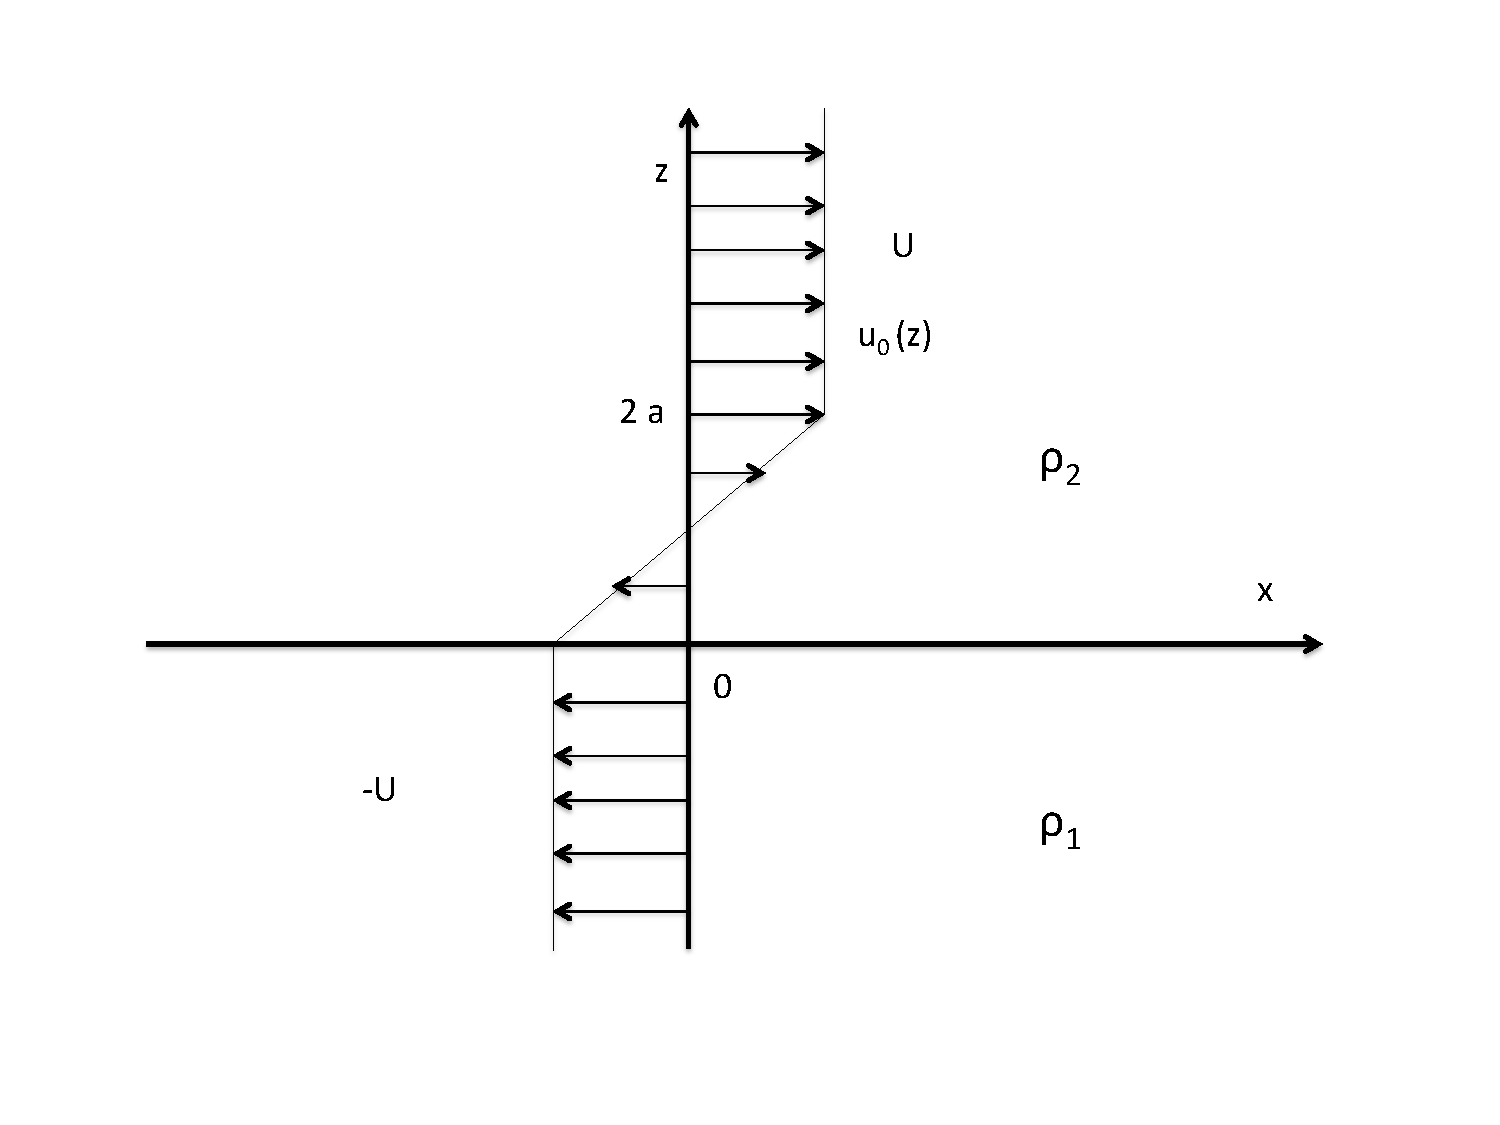
\includegraphics[width=0.8\textwidth]{Figures/2-1.pdf}
\caption{Base velocity profile. \label{khappfig} }
\end{figure}

\subsection{Dispersion relation}

The Euler and incompressibility 
equations are as in Eqs. (\ref{nse1}) with only
$
\LLL =  \LLL_{\rm conv} 
$, surface tension and viscosity are not included.
The interface height $h$ moves according to
\be
\dert h +  u \derx h =  w \label{heq}
\nd
We also use a stream function $\psi$
\be
w = - \derx \psi, \quad u = \dery \psi \label{psiu}
\nd
We consider a small perturbation of the base velocity 
in the form
\be
\U = \U_0  + \eps \U_1 + {\cal O}(\eps^2) \label{1}
\nd
the pressure expands as 
$p=p_0 + \eps p_1(x,z,t) + {\cal O}(\eps^2)$, the height as
$h= \eps h_1(x,z,t) + {\cal O}(\eps^2)$,
and similarly
the stream function. 
We assume the following form for the perturbation
\be
\left(
\ba{c} u_1 \\ w_1 \\ p_1 \\ \psi_1 \\ h_1 \ea \right)
=
\left(
\ba{c} U_1(z) \\ W_1(z) \\ P_1(z) \\ \Psi_1(z) \\ A_h \ea
\right)
e^{- \ii k x - \ii \om t}
\label{UVWdef} \nd
where $k$ is an  arbitrary wavenumber and $\om$ a frequency
to be determined.
Although the expressions on the rhs in (\ref{UVWdef}) are complex we understand the real part.

It is convenient to define
as Chandrasekhar \cite{Chandrasekhar} the reduced wavenumber  $\kappa = 2ka$
and the reduced frequency $\Omega=\om a/U$, which are related by 
\be
e^{-2\kappa} 
=  (1 - 2\Omega - \kappa)\frac{2 + (r+1)(2\Omega - \kappa) }{2+ ({r-1}) (2\Omega - \kappa)},
\label{ev}
\nd
see for example \cite{Eggers08}, equation (135).
The system is unstable whenever Eq. (\ref{ev}) has two complex conjugate non-real roots. Then the positive
imaginary part 
$\Omega_i$ is the growth rate, plotted on Figure \ref{gg1} in the case $r=100$
where $r={\rm max}(\rho_1/\rho_2,\rho_2/\rho_1)$.
The case $r=100$ corresponds to the boundary layer in the gas
and is much less unstable than the case with the boundary layer in the liquid. As the ratio $r$ is increased
the growth rate for the boundary layer in the gas decreases steadily while the growh rate for the boundary layer in the liquid converges to the one for a free surface, with the gas replaced by a void. 
\begin{figure}
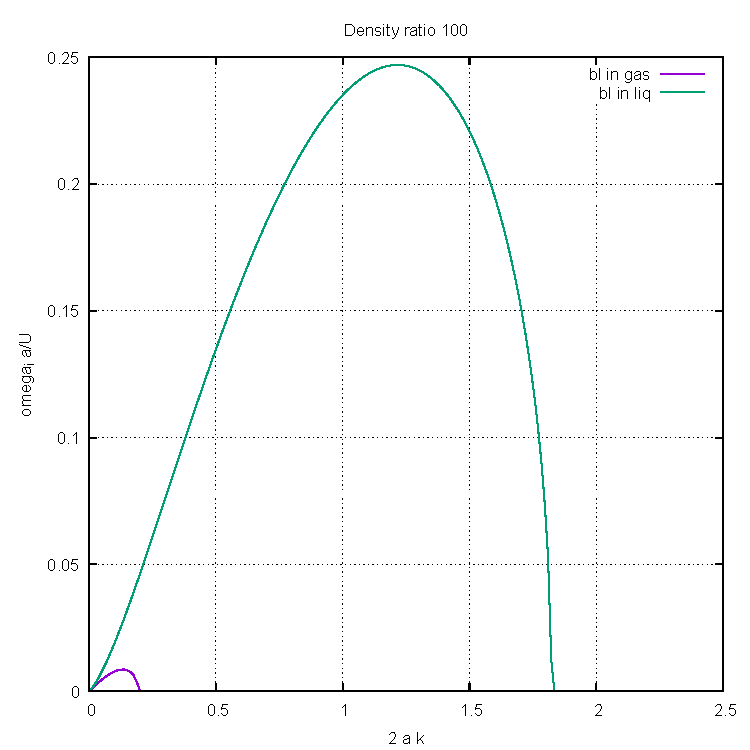
\includegraphics[width=0.8\textwidth]{Figures/rrates_100.pdf}
\caption{Growth rate for $r=100$.  \label{khappfig} }
\end{figure}

\subsection{Special case}

When $a=0$ the above is singular and a special computation
is needed. One has $\kappa=0$ and the frequencies are
\red{
  \be
\om =\left( \frac{r-1}{r+1} +\frac{2 \sqrt r}{r+1}  \ii  \right){ k U } \label{omkaz}
\nd
}

\subsection{Construction of the unstable mode}

We want to write the solution using the stream function $\psi$
in order to have a divergence free initial condition in the computations. 
The construction of $\psi$ is done by determining the relevant coefficients
so that $\psi$ is given by
\blue{
\bea
z<0 & \psi(x,z,t) & =  A_1 e^{kz} e^{-\ii k x - \ii \om t } \label{psi1} \\ 
0 <z< 2a & \psi(x,z,t) & = ( A_0 e^{kz} +  B_0 e^{-kz})  e^{-\ii k x - \ii \om t }  \label{psi2} \\
2a<z & \psi(x,z,t) &=  B_2 e^{-kz}  e^{-\ii k x - \ii \om t } \label{psi3}
\nda
}
From (\ref{heq}) 
\be
\dert h =  -U_0(0) \derx h + w \label{htw}
\nd
and from \refeq{psiu} and  \refeq{psi2} 
we get
$$
- \ii \om  A_h = -\ii k U  A_h +  \ii k (A_0 + B_0)
$$
hence
$$
(- \ii \om + \ii k U)  A_h =  \ii k (A_0 + B_0)
$$
and
$$
A_h = - \frac{k}{\om-kU} (A_0 + B_0) 
$$
Similar relations are obtained from the requirements of continuity of pressure
and normal velocity at $z=0$ and $z=2a$. 
We can then determine all the amplitudes of the constructed solution
after an amplitude for the interface has been chosen. Typically
the modulus $|A_h|$  and the argument $\phi$ are selected so that
$$A_h = | A_h | e^{\ii \phi}$$
then for $\kappa>0$ we have
\red{
\bea
C_0 & = & - (\frac{\om}k- U)A_h ( e^{-2\kappa}  +  2\Omega + \kappa - 1 )^{-1} \label{AhC0}\\
A_0 &=& C_0  e^{-2\kappa}\\
B_0 &=& C_0 (2\Omega + \kappa - 1 ) \label{AB0sol}\\
A_1 & = &  A_0 + B_0 \label{A1A0B0}  \\
B_2 & = &  A_0  e^{2 \kappa} + B_0  \label{B2A0B0}
\nda
}
These expressions for the amplitudes together with (\ref{psi1}-\ref{psi3}) are used to
initialize the stream function. The intermediate constant $C_0$ is used to simplify the expressions.

\subsection{Special cases: mode structure for $ka \rightarrow 0$}

\subsubsection{Mode structure for $a>0$ in the limit $a \rightarrow  0$.}

For small or vanishing $a$ and $\kappa$ however the expression \refeq{AhC0} is singular.
Indeed in the limit $\kappa \rightarrow 0$ we also have $\Omega \rightarrow 0$ and
$$
e^{-2\kappa}  +  2\Omega + \kappa - 1 = - 2\kappa + 2\kappa^2 +   \kappa + \Order(\kappa^3) = - \kappa + \Order(\kappa^2)
$$
and then $A_0$ and $B_0$ become spurious as the region $(0,2a)$ vanishes.
From \refeq{AhC0}
$$
C_0 \simeq  - \frac{\om}k  \frac 1 \kappa A_h
$$
and from \refeq{AB0sol}  and  \refeq{B2A0B0} 
$$
B_2 = C_0 (2\Omega + \kappa) \simeq  C_0 \kappa
$$
Thus for $a=0$
\red{
$$
B_2 = - \frac{\om}k  A_h
$$
$$
A_1 =  \frac{\om}k A_h
$$
}
the latter being obtained directly from \refeq{A1A0B0}. Since $B_2 \neq A_1$
there is a $\Order(\eps)$ discontinuity of $\psi$ which results in a jump of $v(x,z,t)$
accross the interface at $z=0$ and a related thin jet $u_1(x,z,t) \simeq \epsilon f(x,t) \delta(z)$.
This is a consequence of placing the interface in the above calculations at $z=0$ instead of
$z=\eps h_1(x,t)$ and it conflicts with the solution obtained classically with the
thin vortex sheet setup (that is, the setup in which $a=0$ is postulated at the beginning). 

\subsection{Mode structure in the $a=0$ case}

We now obtain the mode structure for the classic thin vortex sheet setup. 
In that case we keep only the terms in \refeq{w1} and \refeq{w3}. The velocity continuity condition becomes
\be
h_t = - u h_x + w = - u_0 h_x + w_1 + \Order(\epsilon) \label{ht}
\nd
which replaces \refeq{htw}. Since $h_t$ must have the same expression above and below the interface
\be
[ w  -  h_x u_0 ]=0
\nd
thus $ [ w] = h_x [u_0] = 2 h_x U $ and from  \refeq{w1} and \refeq{w3}
\bea
z<0 & W_1 &= A^\prime_1 e^{kz}  \\ 
z > 0 & W_1 &= B^\prime_2 e^{-kz}
\nda
and from \refeq{ht}
\bea
A^\prime_1 &=&  -\ii (\om - kU) A_h \label{apht}\\
B^\prime_2 &=&  -\ii (\om + kU) A_h \label{bpht}\\
\nda
The pressure equality at $z=0$ leads to
\bea
z<0 &  P_1 &=    \frac{\ii \rho_1}{k^2} (\om - kU) A^\prime_1 k e^{kz}  \\ 
z>0 &  P_1 &=    \frac{\ii \rho_2}{k^2} (\om + kU) B^\prime_2 (- k e^{-kz}) 
\nda
hence introducing $\nu = \om/(kU)$
and from  \refeq{apht} and \refeq{bpht}
\bea
(\nu+1)A_1 - (\nu-1)B_2 & = &0\\
r (\nu-1)A_1 + (\nu + 1)B_2 & = &0\\
\nda
from which one obtains
  \be
\nu = \frac{r-1}{r+1} +\frac{2 \sqrt r}{r+1}  \ii 
\nd
identical to \refeq{omkaz}. Also from \refeq{apht} and \refeq{bpht}
\bea
A_1 &=&    (U - \om/k) A_h \label{aha}\\
B_2 &=&  - (U + \om/k)  A_h \label{ahb}
\nda
These expressions should be used whenever $a \ll A_h$ while the full expressions with the boundary layer
would be valid for  $A_h \ll a$. In both cases $\Delta x \ll {\rm min}(A_h,a)$ may be required. 



\end{document}
\endinput
%%
%% End of file `elsarticle-template-num.tex'.


